% @file   thesis.tex
% @brief  graduation thesis of Shibaura Institute of Technology
% @author Kataoka Nagi al18036[at]shibaura-it.ac.jp
% @date   2021-12-21 15:19:48
% $Version:   1.0
% @parHistory
% add
% Copyright (c) 2021 Kataoka Nagi

\documentclass[12pt,a4j,dvipdfmx]{jreport}
\setcounter{secnumdepth}{5}
\usepackage[dvipsnames, dvipdfmx]{xcolor}
\usepackage[dvipdfmx]{graphicx}
\usepackage{amsmath,amssymb}
\usepackage{comment}
\usepackage{graphicx}
\usepackage{here}
\usepackage{bm}
\usepackage{url}
\usepackage{otf}
\usepackage{multicol}
\usepackage{multirow}
\usepackage[dvipdfmx, hidelinks]{hyperref}
% \usepackage{breakurl}
% \usepackage{pxjahyper}

\renewcommand{\baselinestretch}{1.5}

\renewcommand{\bibname}{参考文献}





\begin{document}


%%%%%%%%%%%%%%%%%%%%%%%%%%%%%%%%%%%%%
% 表紙
%%%%%%%%%%%%%%%%%%%%%%%%%%%%%%%%%%%%%
\begin{titlepage}

\begin{center}

\vspace*{2cm}
\Large 2021 年度 芝浦工業大学 工学部 情報工学科\\

\vspace*{1.0cm}
\Huge 卒 \qquad 業 \qquad 論 \qquad 文\\
\vspace*{2.5cm}

\Large 主張と根拠のクラスタを用いた\\多様な主張を提示するニュース推薦手法の提案

\vspace{4cm}
\begin{tabular}{ll}
\vspace*{2mm}
学籍番号 & \qquad $\mathbf{AL18036}$ \\
\vspace*{2mm}
氏\phantom{  }名 & \qquad 片岡 \quad 凪   \\
\vspace*{2mm}
指導教員   & \qquad 木村 \quad 昌臣
\end{tabular}
\end{center}
\end{titlepage}



% \begin{abstract}
% このファイルは,情報工学科卒業論文の推奨テンプレートである.概要書とは異なり,卒業論文本体のテンプレートはあくまで推奨であるので,このテンプレートを下にして文字サイズや行間などを修正したものを利用しても良く,またこのテンプレートを使わなくても良い.

% この部分の研究概要では,研究背景,解決したい問題,研究目的,提案手法,評価方法,評価の結果について簡潔に書く.
% 概要の有無は任意.
% \end{abstract}


{\makeatletter
\let\ps@jpl@in\ps@empty
\makeatother
\pagestyle{empty}
\tableofcontents
\clearpage}

\setcounter{page}{1} 
\pagestyle{plain}

%%%%%%%%%%%%%%%%%%%%%%%%%%%%%%%%%%%%%%%%%%%%%%%%%%%%%%%%%%%%
% 書式 
%%%%%%%%%%%%%%%%%%%%%%%%%%%%%%%%%%%%%%%%%%%%%%%%%%%%%%%%%%%%
% 図の参照『図\ref{fig_nn}に3層のニューラルネットワークを示す』
% \begin{figure}[H]
% 	\centering
% 	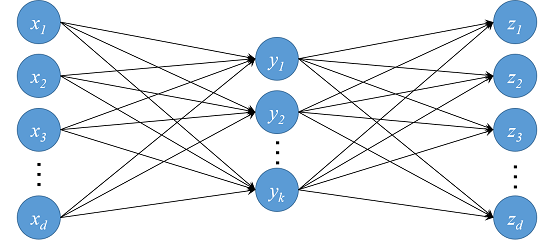
\includegraphics[keepaspectratio, width=120mm]{img/sample.png}
% 	\caption{提案法に用いた3層のニューラルネットワーク.キャプションにはこの図の説明を書く.}
% 	\label{fig_nn}
% \end{figure}

% 表の参照『表\ref{table_a}に手法Aおよび手法Bの正答率を示す』
% \begin{table}[H]
%   \caption{手法Aおよび手法Bの正解率と平均計算時間.}
%   \label{table_a}
%   \centering
%   \begin{tabular}{lcr}
% \hline
% 手法   & 正解率[\%]  &  計算時間[ms]  \\
% \hline \hline
% 手法A  & 92.3  & 512 \\
% 手法B  & 87.4  & 32  \\
% \hline
%   \end{tabular}
% \end{table}

% 参考文献『井尻らは,X線CTとデジタルカメラを用いた3次元モデリング法を提案した\cite{Ijiri18}.』
% 参考文献リスト『著者1, 著者2,...,著者N. タイトル. 論文誌or学会名, 巻, 号, ページ, 発表年. 』
% Webページ『著者. ページタイトル. ページURL(2021年7月31日参照).』


%%%%%%%%%%%%%%%%%%%%%%%%%%%%%%%%%%%%%%%%%%%%%%%%%%%%%%%%%%%%
\chapter{\textcolor{red}{序論}}
%%%%%%%%%%%%%%%%%%%%%%%%%%%%%%%%%%%%%%%%%%%%%%%%%%%%%%%%%%%%

% (用紙や文字のなどのサイズには井尻先生のTeXテンプレートをそのまま利用しています)
% (画像のサイズや\textbackslash newpageのタイミングは最後に調整します)

%%%%%%%%%%%%%%%%%%%%%%%%%%%%%%
\section{研究の背景と目的}

ニュース記事となる出来事は,記者によって受け取り方や伝え方が異なる.
RSF(Reporters Sans Frontières)は,政治や文化などの要因によって記者の主張が制限されていることを問題視している\cite{2021_world_press_freedom_index}.
近年のWebニュースには世界中の記者たちの様々な主張が見られるが,言語の違いによる時間的コストなどから,多くの読者はそれらの主張の一部しか把握できない.
\textcolor{red}{
また,ニュースサイトのアルゴリズムによって読者に合わせて読者の読む記事が選別されているため,選別されなかった記事の主張を読者が把握することは難しい
\cite{pariser_beware_nodate}\cite{bruns_filter_2019}.
}

Yangらは,ニュース読者が出来事を正確かつ迅速に把握できるように
階層的クラスタリングを用いて記事に対するツイートの主張をグループ化する手法を提案した\cite{yang_scalable_2021}.
この研究ではCOVID-19の話題に限定した主張の文をグループ化しているが,この手法を記事に適用した場合,多くの話題について主張のまとまりが生成されることになる.
これでは,COVID-19の飲み薬やワクチンなど異なる話題に含まれる安全性に関する共通した
主張がグループ化されるため,読者が興味を持っている出来事の異なる主張の収集に時間を要してしまう.
% これにより,ニュース読者の正確かつ迅速な出来事の把握の支援を目指す.
% 異なる話題の似た主張をグループ化するエラーに繋がりやすいと考えられる.

% ワクチン 感染 病床 旅行 政治 制作 感染者数 症状 副反応
% 安全性 危険性 予防 

% 近いグループに正確さ
% カテゴリをCOVID-19に限定させたニュースだけでも
% ノイズとなり得る
% Web上には世界の無数の記事には対応できない
% クラスタ数がいうほど減っていない

そこで本研究では,まず世界の記事を出来事の類似度を用いてグループ化し,同じグループの記事群から主張の類似度を用いて再度グループ化することによって,類似した出来事の異なる主張の文を提示する手法を提案する.
\textcolor{red}{提示した主張の文に加え,文の抽出元である記事を推薦する手法についても検討した.}
% これにより,ニュース読者の正確かつ迅速な出来事の把握の支援を目指す.
% ここで,「出来事」は記者の解釈に依存しない事象とし,「主張」は記者が伝えるべきだと判断した出来事の解釈とする.

% @see 

%%%%%%%%%%%%%%%%%%%%%%%%%%%%%%
% \section{研究目的}
% ~
% @see 

%%%%%%%%%%%%%%%%%%%%%%%%%%%%%%
\section{本論文の構成}
本論文は全7章で構成される.
第\ref{chapter_knowledge_and_technologies}章では本研究で用いる知識と技術について説明する.
第\ref{chapter_related_studies}章では本研究と比較する関連研究を紹介し,第\ref{chapter_method}章では関連研究を踏まえた上で提案手法について説明する.
その後,第\ref{chapter_implement}章で提案手法を評価するシステムの実装方法について説明し,第\ref{chapter_experiment}章で説明したシステムを用いた評価実験について述べる.
最後に,第\ref{chapter_conclusion}で本研究の全体を踏まえたまとめと今後の課題を述べる.
% @see 

%%%%%%%%%%%%%%%%%%%%%%%%%%%%%%%%%%%%%%%%%%%%%%%%%%%%%%%%%%%%
\chapter{本研究で用いる知識と技術}
%%%%%%%%%%%%%%%%%%%%%%%%%%%%%%%%%%%%%%%%%%%%%%%%%%%%%%%%%%%%
\label{chapter_knowledge_and_technologies}
%%%%%%%%%%%%%%%%%%%%%%%%%%%%%%
\section{ニュース推薦システム}
多くのWebニュースサイトでは,様々なアルゴリズムを用いて読者の趣向に合わせた記事が提示されている.
アルゴリズムの例として,
読者が閲覧した記事に似た記事を推薦するコンテンツベースフィルタリング(Content-Based Filtering)や
似た趣向を持つ他の読者の閲覧記事を推薦する協調フィルタリング(Collaborative Filtering),
この2つや他のルールを併用したハイブリッドな手法などがある\cite{karimi_news_2018}.
このような読者にパーソナライズした推薦アルゴリズムをニュース推薦システム(News Recommender Systems)という.
アルゴリズムの評価指標には,記事の閲覧回数,閲覧記事のカテゴリ,読者の位置情報,他サイトの閲覧履歴や購買情報などがある.
% @see News recommender systems – Survey and roads ahead

%%%%%%%%%%%%%%%%%%%%%%%%%%%%%%
\subsection{ニュース推薦システムが生むバイアス}
\label{biases_generated_by_nrs}
パーソナライズするニュース推薦システムは,読者が得る情報に偏りを生む.
本節\ref{biases_generated_by_nrs}では,代表的な問題としてフィルターバブル問題とエコーチェンバー問題について記す.
本研究は,両問題の部分的な緩和を目指すものである.
% @see 0517-


\subsubsection{フィルターバブル問題}
Eli Pariserは2011年に,インターネットコンテンツの推薦アルゴリズムにパーソナライズ機能を組み込むことで生じる諸問題をフィルターバブル問題として提唱した\cite{pariser_beware_nodate}\cite{bruns_filter_2019}.
Pariserは,インターネット上で個人の趣向に合わせた限定されたコンテンツばかりが推薦されている状況を,ユーザーが泡の中に閉じ込められたような状態であると例えた.
例として,Facebookでユーザーが支持する政党ばかりが推薦され,Google検索でユーザーの居住地域と関係が薄い時事問題が推薦されるような状況が問題視されている.
泡の中の偏った情報は,新しいアイディアや異なる視点を生みにくくする.
市民が偏った情報ばかりに触れることで,民主主義が機能しなくなる可能性もある.

この泡の中で多様性のある情報を求めることは難しい.
なぜなら,泡の中の情報は個人のキャリアや行動履歴によって決まるため,個人で推薦アルゴリズムをコントロールできないことが多いからである.
同じ理由で,個人が泡の外の情報を特定できないことも大きな問題である.

% (to 提案手法)フィルターバブル問題を緩和する策として,推薦アルゴリズムの公開,個人が推薦アルゴリズムを管理できるオプションの作成,UIの工夫によるバブルの可視化がある.一方で,個人が推薦アルゴリズムを微調節したところで完全に情報の泡から脱することはできないとの指摘もある.UIでバブル内外を可視化しきるのは不可能 情報が多い 手軽

% @see 
% [1]E. Pariser, Beware online 「filter bubbles」, (1304298000). 参照: 1月 06, 2022. [Online Video]. Available at: https://www.ted.com/talks/eli_pariser_beware_online_filter_bubbles
% - きっかけ
%     - Facebook
%         - リベラル派だが進んで保守派と交流する
%         - ある日保守派の人たちが消えた
%         - どのリンクをクリックしているかFacebookがチェック
% - その他の例
%     - Google
%         - 57個のシグナルをチェック
%             - どんなPCを使っているか
%             - どのブラウザを使っているか
%             - 現在地は何処か
%         - 検索結果を調節
%         - 認識しにくい
%             - 自分の検索結果がどれほど他人のものと違うか分からない 
%         - 友人2人がGoogleで「エジプト」と検索
%             - エジプトのデモ関連記事が全くない
%                 - この頃大きな話題だったのに
%             - 他方はそればかり
%     - Yahoo!ニュース,Huffington Post,Washington Post,New York Times
%         - 様々な形でカスタマイズ
% - インターネットは私たちが見たいものを予測して見せている
%     - それは必ずしも見る必要があるものでない
%     - エリック・シュミット「全く何のカスタマイズもされていないものを 人々が見たり利用したりするのは とても難しくなるでしょう」
% - フィルターやアルゴリズムの結果
%     - フィルターに囲まれた世界
%         - あなた個人独特の情報世界となる
%         - 自分の世界に何が含まれるかは自分がどんな人で何をしているかによって決まる
%         - 何が取り入れられるかは自分次第でないのが問題
%             - Netflixのデータアナリスト「「アイアンマン」はすぐ届くのに 「スーパーマン」は 待ち時間が長い」
%                 - 利用者の計画的な向上心と衝動的な今の欲望が大きく対立
%                     - 「羅生門」を観たことがある人になりたい
%                         - 一方で4回目の 「エース・ベンチュラ」を観たい
%                     - 最良の編集は両面を見せる
%                     - フィルターは利用者が何を最初にクリックしたかを主に参考
%                         - そのようなバランスを崩す
%         - **何が削除されるか自分には見えない**
% - 放送社会の創設神話
%     - 編集者が情報の流れをコントロール
%     - インターネットが現れ編集者を追い払った
%     - 私たちは 繋がり合えるようになった
%         - 実際にはそうなっていない
%         - 人間の門番からアルゴリズムの門番にバトンが渡されている
%         - **アルゴリズムは編集者が持ち合わせていた倫理観念をまだ持っていない**
%             - アルゴリズムが関連性以外の要素も必要
%                 - 私たちが何を見て何を見ないか決めるのなら.
%             - 見たくないものや難しいもの,重要なものなども提示
% - 1915年
%     - 新聞は市民としての義務は考慮しない
%     - 市民が適切な情報を得ていないと民主主義は機能しない
%     - 情報のフィルターを行う新聞は重要
%         - ジャーナリズムの倫理が誕生
%     - ウェブ上で同じ問題に直面
%     - プログラムにこの責任を組み込みたい
%         - アルゴリズムを明白に
%         - 何が入ってくるか
%         - フィルターのルール
%         - 自分で何が削除されて何がされないか決められるように管理できるオプション
%         - 新しいアイデアや人々,異なる視点を提示すべき
%         - ウェブ上で私たちが孤立しないように
% [1]和俊笹原, 「ウェブの功罪」, 情報の科学と技術, vol. 70, no. 6, pp. 309–314, 2020, doi: 10.18919/jkg.70.6_309.
% - パーソナライゼーション
% - 選択の条件を知り得ない
% - ブラックボックスであることも
% - **アルゴリズムで虚偽情報が組み込まれることも**
% [1]亜斗夢園田, 寛人中島と不二夫鳥海, 「人気度に着目したニュース閲覧行動の変容分析」, 人工知能学会全国大会論文集, vol. JSAI2020, p. 1L5GS501-1L5GS501, 2020, doi: 10.11517/pjsai.JSAI2020.0_1L5GS501.
% - 自らが好む情報やそれを支持するコミュニティばかり接触することで,偏った考えがより強化される現象
% [1]敏弘神嶌, 昭太郎赤穂, 英樹麻生と淳佐久間, 「情報中立推薦システム」, 人工知能学会全国大会論文集, vol. JSAI2012, p. 3E1R61-3E1R61, 2012, doi: 10.11517/pjsai.JSAI2012.0_3E1R61.
% - フィルターバブル
%     - 利用者が接する情報の範囲に関する問題
%     - 推薦などの個人化技術により,利用者は,知らないうちに,自身が関心があるとされる限定された話題の情報のみにしか接しないようになっており,まるで『泡』の中に閉じ込めらたような状態
%     - 利用者がより新たな話題に関心をもつ機会が奪われたり,社会の中での情報や認識の共有が困難に
%     - フィルターバブル
%     - 推薦を含めた個人化技術によって
%     - 利用者が接する情報の話題の範囲が狭められたり,偏ったりすることが
%     - 利用者が知らないうちに行われるという問題
% [[1]E. BozdagとJ. van den Hoven, 「Breaking the filter bubble: democracy and design」, Ethics Inf Technol, vol. 17, no. 4, pp. 249–265, 12月 2015, doi: 10.1007/s10676-015-9380-y.](https://link.springer.com/article/10.1007/s10676-015-9380-y?source=post_page-----2afbf9cd8367----------------------)
% -  FB
%   -  情報の質の低下
%   -  多様性の低下
% [1]A. Bruns, 「Filter bubble」, Internet Policy Review, vol. 8, no. 4, 11月 2019, 参照: 5月 29, 2021. [Online]. Available at: https://policyreview.info/concepts/filter-bubble
% - フィルターバブル
%     - Eli Pariserが2011年に提唱した概念
%     - 中立的,多様かと思いきや偏っていく
%     - 明確な定義はない
% - 本稿の定義
%     - フィルターバブル
%         - 参加者のグループが,部外者を排除して,お互いに優先的にコミュニケーションをとることを選択したときに発生する(例:Facebookでのコメント,Twitterでの@mentionsなど
%         - 最適化をコントロールしようとする努力もフィルターバブル
% [1]S. NagulendraとJ. Vassileva, 「Understanding and controlling the filter bubble through interactive visualization: a user study」, Proceedings of the 25th ACM conference on Hypertext and social media, New York, NY, USA, 9月 2014, pp. 107–115. doi: 10.1145/2631775.2631811.
% - FBのメリット
%     - 得る速さ
%     - オーバーロードの少なさ
% - FBのデメリット
%     - 偏りに気付かない
%     - 重要だが好き嫌いのある情報が隠れる
%     - ユーザは面白いものにばかりコメントし,囲まれる
%         - 考えさせられる情報
%         - 新しい情報
%     - 開発者に制御される
% - カテゴリのバブル
%     - カテゴリの一般性は高く
%         - 実用上?
%     - Aさんが閲覧した友人Bさんの投稿の1週間のカテゴリービュー
%         - 表示されたらバブル内
%         - Aさんが興味がない可能性
%         - AさんがBさんに共感していない可能性
%         - 過去のいいねした内容に基づく
% - 人間関係のバブル
%     - 逆に,カテゴリーに反応した友人を表示
% [1]広志古賀, 「フィルターバブルとマス破壊兵器について」, 情報経営, vol. 80, pp. 63–66, 2020, doi: 10.20627/jsimconf.80.0_63.
% - フィルターバブル
%   - インターネットの検索履歴がフィルターとなり,同じような情報ばかり表示される(見たくない情報を遮断する)こと
% - フィルターバブル
%     - 無関心圏を拡大
%     - 貢献と誘因の葛藤を放棄
% [1]雅裕片岡, 智訓橋山と俊一田野, 「フィルターバブルを気づかせるシステムの提案」, 人工知能学会全国大会論文集, vol. JSAI2015, pp. 1H21-1H21, 2015, doi: 10.11517/pjsai.JSAI2015.0_1H21.
% - FB
%     - > 推薦システムの発達により利用者が触れる情報は利用者の好みに合う情報ばかりになり,知らず知らずのうちに利用者の興味外の情報や新しい情報などに触れる機会が失われるようになった状態
%     - 社会的リアリティの共有の困難
%     - イデオロギーの極性化
%     - 創造性の低下
% - 問題例
%     - Facebook feed
%         - あまり見てない保守派が突然アルゴリズムで消された
%     - Google検索
%         - 友人に検索させる
%         - 時事的なのエジプト革命でなく,旅行ばかり
% [1]明子小川, 「分断の時代におけるナラティヴとストーリーテリング教育」, 言語文化教育研究, vol. 16, pp. 45–54, 2018, doi: 10.14960/gbkkg.16.45.
% - フィルターバブル
%     - 似た意見や関心を持った人々との間でのみ交流を続ける


\subsubsection{エコーチェンバー問題}
SNS上で価値観の似た者同士が交流し,共感し合うことにより,偏った意見や思想が反響室のように増幅されて影響力をもつ問題をエコーチェンバー問題という\cite{bruns_filter_2019}
% \cite{inc_echo_nodate}
\cite{nguyen_echo_2020}.
Conoverらや笹原和俊らは,アメリカの選挙期間中のTwitterユーザーが自身の支持する政党に関するツイートを多くリツイートしており,エコーチェンバー問題が生じていることを確認した\cite{conover_partisan_2012}\cite{__2020-5}.

エコーチェンバーの中では,SNSユーザーは自身と異なる価値観や考え方を持つユーザーと交流する機会を失い,偽の情報を訂正する情報を得にくくなってしまう問題もある\cite{__2020-5}.
近年のニュースは読者でコメントを交わすSNSのような性質を有しており\cite{nagulendra_understanding_2014},エコーチェンバーによる情報の偏りを生むと考えられる.
% (to 提案手法)特定の地域の似た文化と価値観を持つ者同士に向けて記事を提供し,読者にコメントさせる事は,エコーチェンバー問題による情報の偏りを生むと考える.

% [5]亜斗夢園田, 喜史関と不二夫鳥海, **「オンラインメディア記事の読者の行動分析」**, 人工知能学会全国大会論文集, vol. JSAI2019, p. 1I2J504-1I2J504, 2019, doi: 10.11517/pjsai.JSAI2019.0_1I2J504.
% - 異なる意見に対する寛容性の低下
% - マイノリティへの偏見の増大
% - フェイクニュースの無批判な受容

% @see 
% [1]和俊笹原, 「ウェブの功罪」, 情報の科学と技術, vol. 70, no. 6, pp. 309–314, 2020, doi: 10.18919/jkg.70.6_309.
% - 似た価値観や考え方をもつユーザーばかりをフォローし,閉じた情報環境ができること
% - 何度も同じ情報を見聞きし,単純接触効果で信じやすくなる
% - 異なる視線のデマ訂正が見えない
% [1]亜斗夢園田, 寛人中島と不二夫鳥海, 「人気度に着目したニュース閲覧行動の変容分析」, 人工知能学会全国大会論文集, vol. JSAI2020, p. 1L5GS501-1L5GS501, 2020, doi: 10.11517/pjsai.JSAI2020.0_1L5GS501.
% - 過度の推薦によってユーザに偏った情報のみを提供し広い視野が失われる現象
% [1]A. Bruns, 「Filter bubble」, Internet Policy Review, vol. 8, no. 4, 11月 2019, 参照: 5月 29, 2021. [Online]. Available at: https://policyreview.info/concepts/filter-bubble
% - 本稿の定義
% - エコーチェンバー
%         - 参加者のグループが,外部の人間を排除して,優先的にお互いにつながることを選択したときに発生する(例:Facebookで友達になる,Twitterでフォローするなど).
% [1]広志古賀, 「フィルターバブルとマス破壊兵器について」, 情報経営, vol. 80, pp. 63–66, 2020, doi: 10.20627/jsimconf.80.0_63.
% - エコーチェンバー現象
%     - 閉塞空間では,見たい情報しか見えないという状況が生まれる傾向が強い
%     - そのために,特定の信念が増幅または強化され,反対意見を受け容れ難くなる
% [1]明子小川, 「分断の時代におけるナラティヴとストーリーテリング教育」, 言語文化教育研究, vol. 16, pp. 45–54, 2018, doi: 10.14960/gbkkg.16.45.
% - エコーチェンバー
%     - 同じような考えや嗜好の人々の間で意見が反響
% [1]Nguyen, C. T. (2020).   Echo Chambers and Epistemic Bubbles Episteme, 17(2), 141-161.
% - 認識論的バブル
%     - 他者の声が欠落によって除外された情報ネットワーク
%     - 不健全なNW
% - エコーチェンバー
%     - 他者の声が積極的に信頼されなくなった社会的構造
%     - 健全なNWにも存在可能
%     - はるかに脅威
%         - 明白な証拠に対する激しい抵抗を説明できる
% - 選択的暴露
%     - 同じ考えをもつ人から情報を得ようとする行為者の傾向
% - 行為者の情報環境は他の行為者によって改変され得る
%     - フィルター技術
%         - アルゴリズムの秘匿性のため,ユーザーは検索結果が調整される度合いを過小評価
%         - フィルターバブルはフィルター技術に限定

% \subsection{エピステミックバブル}

%%%%%%%%%%%%%%%%%%%%%%%%%%%%%%
\section{機械学習の基礎}
機械学習は,コンピュータにデータを学習させるコンピュータープログラミングに関する科学技術である\cite{aurellen20}.
ここでいう「学習」は,コンピュータに与えたタスクについて,その評価指標が向上するようなコンピュータープログラミムを実行することを指す.
機械学習を用いることで,既知のアルゴリズムが無い問題を解決したり,データの予想外な傾向を発見したりすることができる.
また,僅かに異なる複数のデータごとにアルゴリズムを用意せずとも実行できる強みをもつ.
以下では,本研究に関連する機械学習に関する知識について記す.


\subsection{教師あり学習}
教師あり学習は,データにラベルと呼ばれる出力の答えの情報を付与する機械学習である\cite{aurellen20}.
ラベルは人間の関与の基に設定されることが多い.

本研究で行うクラス分類は教師あり学習のひとつである.
クラス分類ではクラスのラベルを基にデータの特徴とクラスの関係を学習し,新規にモデルに入力されたデータがどのクラスに属するかの確率を出力する.
% @see 

\subsection{教師なし学習}
教師なし学習は,データにラベルを付与しない機械学習である\cite{aurellen20}.
人間が関与した答えを用いずにデータの傾向を分析する.

本研究で行うクラスタリングは教師なし学習のひとつである.
クラスタリングでは,データの特徴を基に似たデータ同士をクラスに振り分ける.
データの何を特徴とし,何を基に似たデータと判断するかが重要で,目的によって工夫する必要がある.

%%%%%%%%%%%%%%%%%%%%%%%%%%%%%%

\section{ニューラルネットワーク}
図\ref{fig_nn}に示すニューラルネットワークは,動物の脳細胞からヒントを得た機械学習の基本的なモデルである\cite{aurellen20}.
式(\ref{nn_layer})に示すように,複数の入力から1つ以上の出力を得る関数や,この関数をいくつか合成させた関数で表される.
図\ref{fig_nn}の個々の円をノード,左端のモデルの入力を受け取るノード群を入力層,右端のモデルの出力を担うノード群を出力層と呼ぶ.
また,入力層と出力層の間に位置する縦1列のノード群を中間層(隠れ層)という.
中間層のうち,前後の層の全てのノードと接続する層を全結合層という.

\begin{figure}[H]
	\centering
	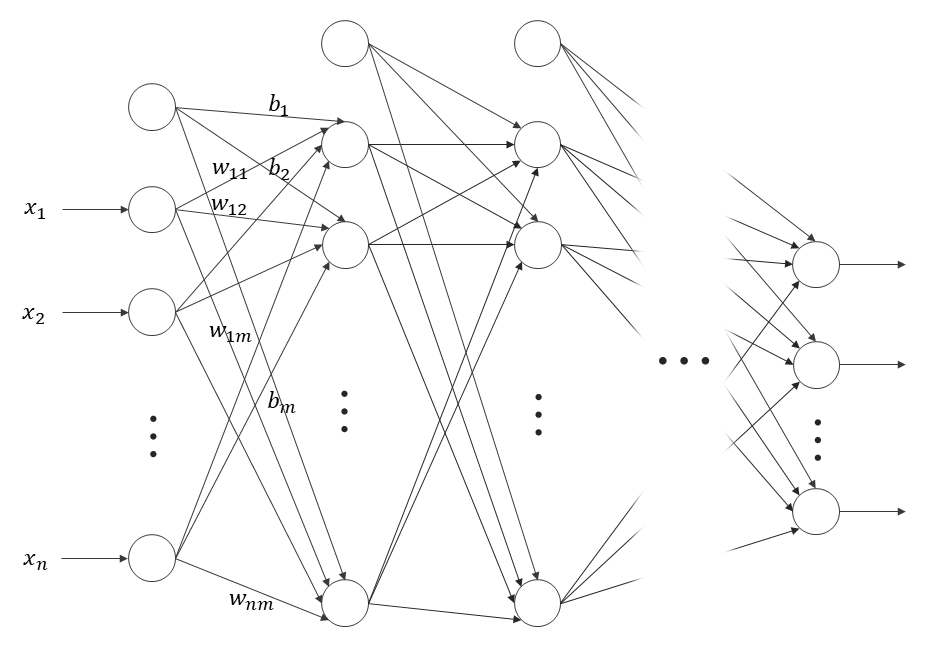
\includegraphics[keepaspectratio, width=120mm]{img/nn.png}
	\caption{ニューラルネットワークのモデルアーキテクチャ}
	\label{fig_nn}
\end{figure}

\begin{align}
  \bm{h}_{\bm{W},~ \bm{b}}(\bm{X}) &= \bm{\phi}(\bm{X}\bm{W} + \bm{b}) \label{nn_layer}
  \\
  \nonumber
  \\
  \bm{X} &= 
  \begin{bmatrix}
    & x_1 & x_2 & \cdots & x_n  &
  \end{bmatrix}
  \label{nn_x}
  \\
  \nonumber
  \\
  \bm{W} &=
  \begin{bmatrix}
    & w_{11} & w_{12} & \cdots & w_{1m} & \\
    & w_{21} & w_{22} & \cdots & w_{2m} & \\
    & \vdots & \vdots & \ddots & \vdots & \\
    & w_{n1} & w_{n2} & \cdots & w_{nm} & \\
  \end{bmatrix}
  \label{nn_w}
  \\
  \nonumber
  \\
  \bm{b} &=
  \begin{bmatrix}
    & b_1 & b_2 & \cdots & b_n  &
  \end{bmatrix}
  \label{nn_b}
\end{align}

$\bm{X}$は数値化したデータの特徴を示す特徴量,
$\bm{W}$はノード間の関係の強さを示す接続重み,
$\bm{b}$は一般に1を要素とするバイアスニューロンと呼ばれるものである.

ニューラルネットワークは脳細胞と似たように,個々のノード間の関係の強さを調節して機能する.
具体的には,式(\ref{nn_update_weight})に示すようにノードの理想の出力$\hat{y}_j$と実際の出力$y_j$の差\textcolor{red}{や次節\ref{subsection_loss_function}で説明する損失関数$L$}を利用するなどして次の学習時の接続重みを更新する.

\begin{align}
  w_{i, j}^{(next~ step)} &= w_{i, j} + \eta~ (y_j - \hat{y}_j)~ \color{red}{\frac{\partial L}{\partial w_{i, j}}}
  \label{nn_update_weight}
  \\
  \eta &= Const.
  \label{nn_learning_rate}
\end{align}
% @see @.289

種々のタスクに特化した機械学習モデルは,このニューラルネットワークの各ノードの接続方法や追加の関数を工夫して作成される.

\subsection{損失関数}
\label{subsection_loss_function}
損失関数は,機械学習モデルの出力層の出力と正解の出力との誤差を表す関数であり,モデルの学習ごとの性能指標として用いられる\cite{aurellen20}.
本研究のクラス分類では,2クラスの分類によく用いられる損失関数として
% 式\ref{mse}に示す平均二乗誤差
式(\ref{binary_cross_entropy})に示す
\textcolor{red}{バイナリクロスエントロピー(BCE)}
を用いた.

% \begin{align}
%   MSE\left(\bm{X}^{\left( i \right)}, h \right)
%   &= \frac{1}{m} \sum_{i=1}^m 
%   \left\{
%     h \left( \bm{X}^{\left( i \right)} \right)
%     -
%     \hat{y}^{\left( i \right)}
%   \right\}^2
%   \label{mse}
% \end{align}

% $h \left( \bm{X}^{\left( i \right)} \right)$
% はモデルの出力,
% $\hat{y}^{\left( i \right)}$
% は正解の出力を表し,
% m個のデータについてこれらの差の二乗の平均を求めて誤差としている.

\begin{align}
  \color{red}{L}(\theta)&=-\frac{1}{m} \sum_{i=1}^{m}\left[y_{i} \log \left(\hat{p}_{i}\right)+\left(1-y_{i}\right) \log \left(1-\hat{p}_{i}\right)\right]
  \label{binary_cross_entropy}
  \\
  % \hat{y}&=\left\{
  % \begin{array}{ll}
  %   0 & \text { if } \hat{p}<0.5 \\
  %   1 & \text { if } \hat{p} \geqq 0.5
  % \end{array}\right.
  % \label{logistic_predict}
  y_{i}&=\left\{
    \begin{array}{l}
      0 \\
      1 
    \end{array}
  \right.
  \label{logistic_predict}
  \\
  \hat{p}
  &=\left[ \hat{p}^{(1)}~ \hat{p}^{(2)}~ \cdots~ \hat{p}^{(m)} \right]
  =h_{\theta}(\mathbf{x})
  =\sigma\left(\mathbf{x}^{\top} \theta\right)
  \label{logistic_probability}
  \\
  \sigma(t)&=\frac{1}{1+\exp (-t)}
  \label{sigmoid}
\end{align}

$y_{i}$は入力する特徴$\mathbf{x}$の個々の要素のラベルで,$\hat{p}$は$\mathbf{x}$の個々の要素についてモデルが予測したラベルが1となる確率である.
\textcolor{red}{バイナリクロスエントロピー$L(\theta)$}は個々の$y_{i}$と$\hat{p}_{i}$の差が大きいほど大きくなり,この差が小さいほど0に漸近する.
式(\ref{logistic_probability})の$\theta$は特徴$\mathbf{x}$のどの要素を重視するかを設定する重み係数である.
式(\ref{sigmoid})の$\sigma(t)$はシグモイド関数と呼ばれる連続関数であり,実数tを入力したとき図\ref{fig_sigmoid}のように確率の範囲$(0, 1)$で実数を出力する.シグモイド関数を用いることで,$(0, 1)$の範囲にないモデルの出力を$(0, 1)$の範囲に落とし込むことができる.

% $h \left( \bm{X}^{\left( i \right)} \right)$
% はモデルの出力,
% $\hat{y}^{\left( i \right)}$
% は正解の出力を表し,
% m個のデータについてこれらの差の二乗の平均を求めて誤差としている.
ニューラルネットワークの重みの更新は損失関数を基に行われ,勾配降下法や誤差逆伝播法を用いて効率よく計算される.
% シグモイド関数は微分をしやすく,勾配降下法や誤差逆伝播法に用いやすい.

\begin{figure}[H]
  \centering
  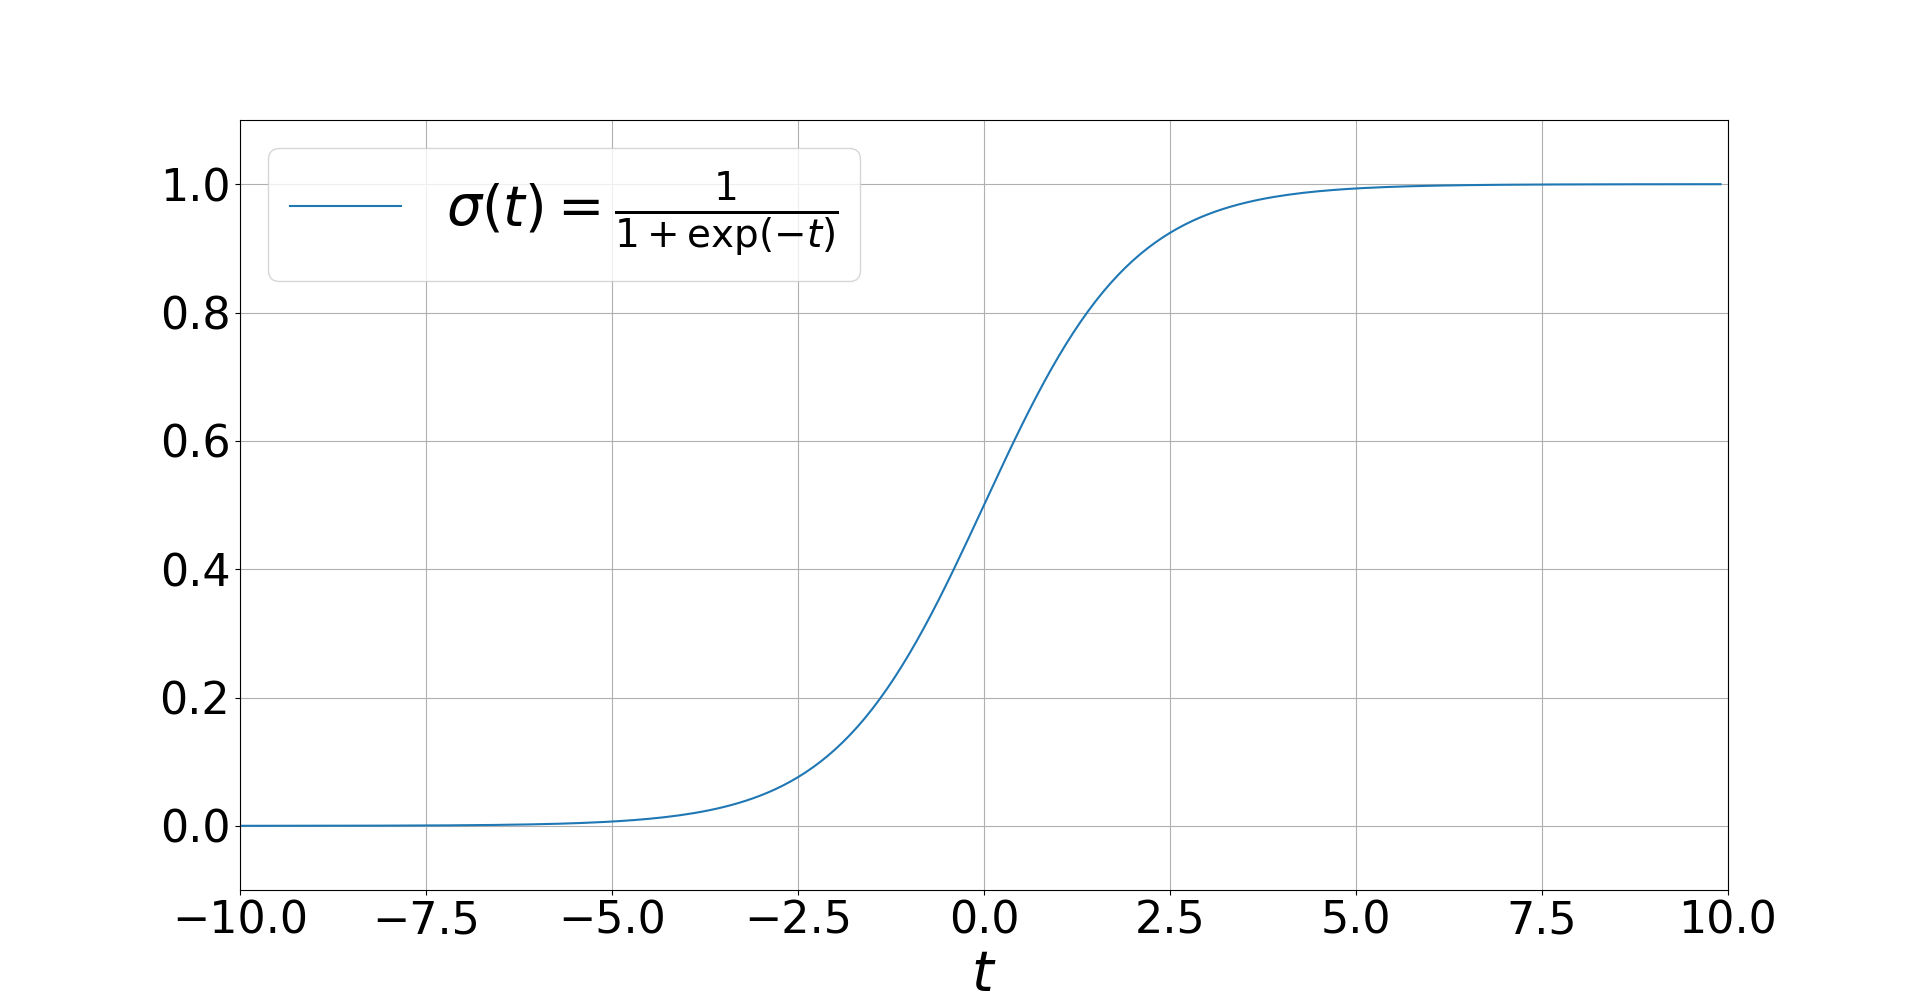
\includegraphics[keepaspectratio, width=120mm]{img/sigmoid.png}
  \caption{シグモイド関数}
  \label{fig_sigmoid}
\end{figure}

% @see p.41, 115

% \subsection{勾配降下法}
% 勾配降下法は,

% @see 4.2 p.~~90~~, 119-139, 174
% 勾配降下法も最適化の話なので省略可能
% 誤差逆伝播法は勾配降下法の効率化なので省略可能 290-294

%%%%%%%%%%%%%%%%%%%%%%%%%%%%%%

\section{機械学習の文章データへの応用}
\label{apply_for_time_series_data}
日々の気温や株価,Webサイトのアクセス数のように,時刻ごとに計測されるデータを時系列データという\cite{aurellen20}.
上記の例では,過去のデータの傾向から未来のデータを予測することができる.
特に,予測したい時刻$t$のデータの直前のデータは,時刻$t$のデータに類似していたり時刻$t$周辺のデータの変化率の情報を含んでいたりするため,予測に大きく役立つ.

時刻を文章内の単語の順番に対応させると,文章データも時系列データと見なすことができる.
文章内の任意の単語は,その前後の単語の意味や文法の傾向から予測することができる.
特に,予測したい単語の直前・直後の単語は,単語の予測の大きなヒントとなる.

本節\ref{apply_for_time_series_data}では,文章をはじめとした時系列データを分析するための機械学習の応用例について記す.
% @see 

\subsection{単語埋め込み}
データのカテゴリを表現する訓練可能な密なベクトルを埋め込みという\cite{aurellen20}.
中でも,単語や文を表現しようとする埋め込みをそれぞれ単語埋め込み,文埋め込み呼ぶ.

デフォルトでは,ベクトルは無作為な数値で初期化される.
例えば,\textcolor{red}{``}NEAR BAY\textcolor{red}{''}というカテゴリは,\textcolor{red}{初期状態で無作為な値を成分にもつ}ベクトルで表現される.
ベクトルの次元数は,目的やモデルの構造によって調節する必要がある.
初期化した単語埋め込みは,意味が似た単語の埋め込み同士は距離を小さくするなど,何らかのアルゴリズムで表現を学習していく.
学習した表現が適切であるほど,単語埋め込みを利用した自然言語処理の機械学習タスクはより精度が増す.
% $v(King) - v(Man) + v(Woman) = v(Queen)$といった加算・減算ができるようになる.
% @see p.430

\subsection{テキストの前処理}
\label{subsection_texts_preprocessing}
単語埋め込みのように,自然言語処理ではテキストをコンピュータが解釈しやすい数値に変換して処理することが多い.
このとき,コンピュータはテキストを文字の羅列としか見ていないため,Appleとappleを別の単語と見なし,違う数値に変換してしまう.
このような単語の表記揺れは,文章中の単語の出現頻度の情報を不正確なものにする.
表記揺れによって増加した出現頻度の少ない単語が学習のノイズとなってしまうこともある.
従って,テキストに何らかの処理をする前に,大文字を小文字に変換するなどの表記揺れを解消する処理を行う必要がある.
URLやメールアドレスといったユニークな文字の羅列は,出現頻度が極めて少ないノイズとなり得るため,事前に除去しておくと良い.

% @see 週次報告書 2021年10月13日
% @see [自然言語処理における前処理の種類とその威力(2017)](https://qiita.com/Hironsan/items/2466fe0f344115aff177)

\subsection{Attention}
Bahdanauらが2014年に提案したAttentionは,時系列データの機械学習を行う際,出力データと関わりが強い入力データに効率よく比重を与える\textcolor{red}{仕組み}である\cite{aurellen20}\cite{bahdanau_neural_2016}.
モデルにAttentionを組み込むことで無駄なデータの学習が減り,モデルが過去に学習した内容を忘却しにくくなる.
これにより,30語以上の長い文章の機械翻訳タスクの精度が大幅に向上する.

図\ref{fig_attention}に機械翻訳モデルに組み込まれたAttention機構を示す.

\begin{figure}[H]
	\centering
	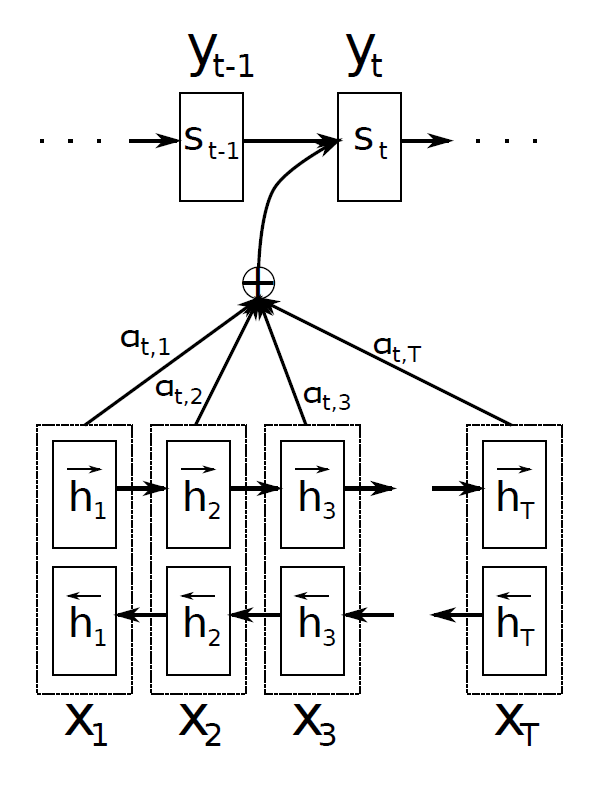
\includegraphics[keepaspectratio, width=50mm]{img/attention.png}
	\caption{入力単語群$(x_1, x_2, ... , x_T)$を基にt番目の出力語$y_t$を生成するAttentionのモデルアーキテクチャ
  \protect\footnotemark[1]
  \textcolor{red}{make width smaller}
  }
	\label{fig_attention}
\end{figure}
\footnotetext[1]{\cite{bahdanau_neural_2016}より引用}

直前に翻訳した単語$y_{t-1}$と過去に翻訳した単語群の情報$s_{t-1}$に,Attentionの式\textcolor{red}{(\ref{attention_c})}を考慮して次の単語$y_t$を予測している.
$\vec{h_i}$は文脈を加味した単語の意味情報をもつベクトルであり,BiGRUと呼ばれるニューラルネットワークを用いて生成されている.

\begin{align}
  c_{i} &= \sum_{j=1}^{T_{x}} \alpha_{i j} h_{j} &
  \label{attention_c}
  \\
  \alpha_{i j} &= \operatorname*{softmax}_j(e_{ij}) = \frac{\exp \left(e_{i j}\right)}{\sum_{k=1}^{T_{x}} \exp \left(e_{i k}\right)}
  \label{attention_alpha}
  \\
  e_{i j} &= a\left(s_{i-1}, h_{j}\right) = v_{a}^{\top} \tanh \left(W_{a} s_{i-1}+U_{a} h_{j}\right)
  \label{attention_e}
\end{align}

式(\ref{attention_alpha})はソフトマックス関数と呼ばれる関数に式(\ref{attention_e})を代入したものであり$\sum_j \alpha_{ij} = 1$となる意味ベクトル$h_j$の重み係数を表す.
式(\ref{attention_e})は,過去に翻訳した単語群の情報$s_{t-1}$と入力単語の意味ベクトル$h_j$を基に,どの単語に比重を置くかを決定するニューラルネットワークである.
式(\ref{attention_e})の$v_{a}^{\top},~ W_{a},~ U_{a}$はニューラルネットワークの重みである.

\subsection{Transformer}
Vaswaniらが2017年に提案したTransformerは,Attentionを組み込んだ翻訳タスクに用いられる機械学習モデルで,2017年の最先端のモデルと比べて数分の1のコストで最大級の精度を有する\cite{aurellen20}\cite{vaswani_attention_nodate}.
時系列データを扱う従来の機械学習にはRNN(Recurrent Neural Network)が多く組み込まれていたが,このモデルは単語を逐次的に処理する仕組みになっており,並列演算が難しい.
一方でTransformerは,RNNを組み込まずに並列演算が可能なAttentionを多く組み込んで時系列データを処理するため,処理コストが低い.

Transformerは,文章を文意を表すベクトルに変換するエンコーダ部分と,そのベクトルを用いて目的の文章を生成するデコーダ部分に分かれるエンコーダ・デコーダモデルの一種である.
図\ref{fig_transformer}に示すTransformerのうち,左半分がエンコーダ,右半分がデコーダである.
エンコーダの入力は翻訳前の文章であり,デコーダの入力はエンコーダの出力と翻訳後の文章である.
デコーダの出力は翻訳中の文章の次の単語の予測確率である.
なお,デコーダに入力される翻訳後の文章は,モデルの学習の際には全文が渡され,予測の際には翻訳中の単語群が渡される.

\begin{figure}[H]
	\centering
	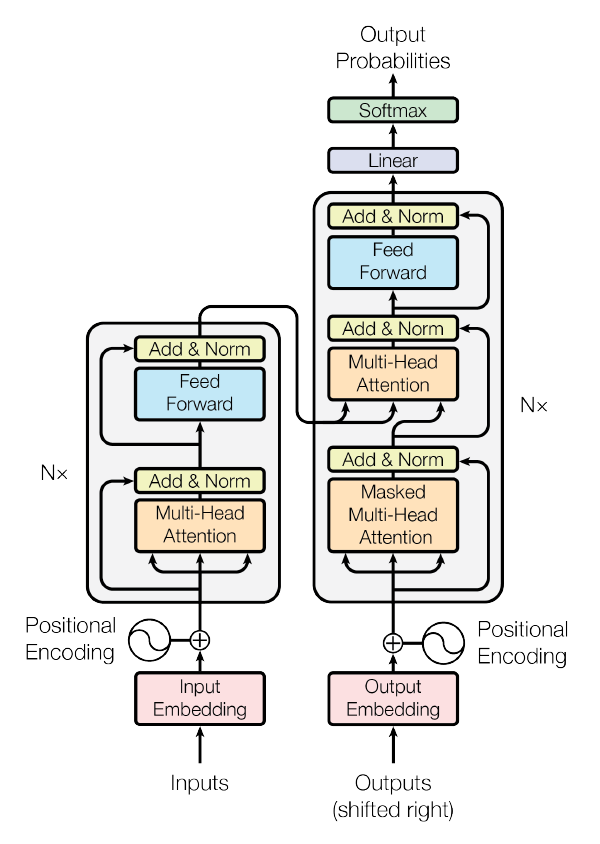
\includegraphics[keepaspectratio, width=120mm]{img/transformer.png}
	\caption{Transformerのモデルアーキテクチャ\protect\footnotemark[2]}
	\label{fig_transformer}
\end{figure}
\footnotetext[2]{\cite{vaswani_attention_nodate}より引用}

Transformerの学習コストを低減する所以となるAttentionは,図\ref{fig_attentions-of-transformer}のように工夫されて組み込まれている.

\begin{figure}[H]
	\centering
	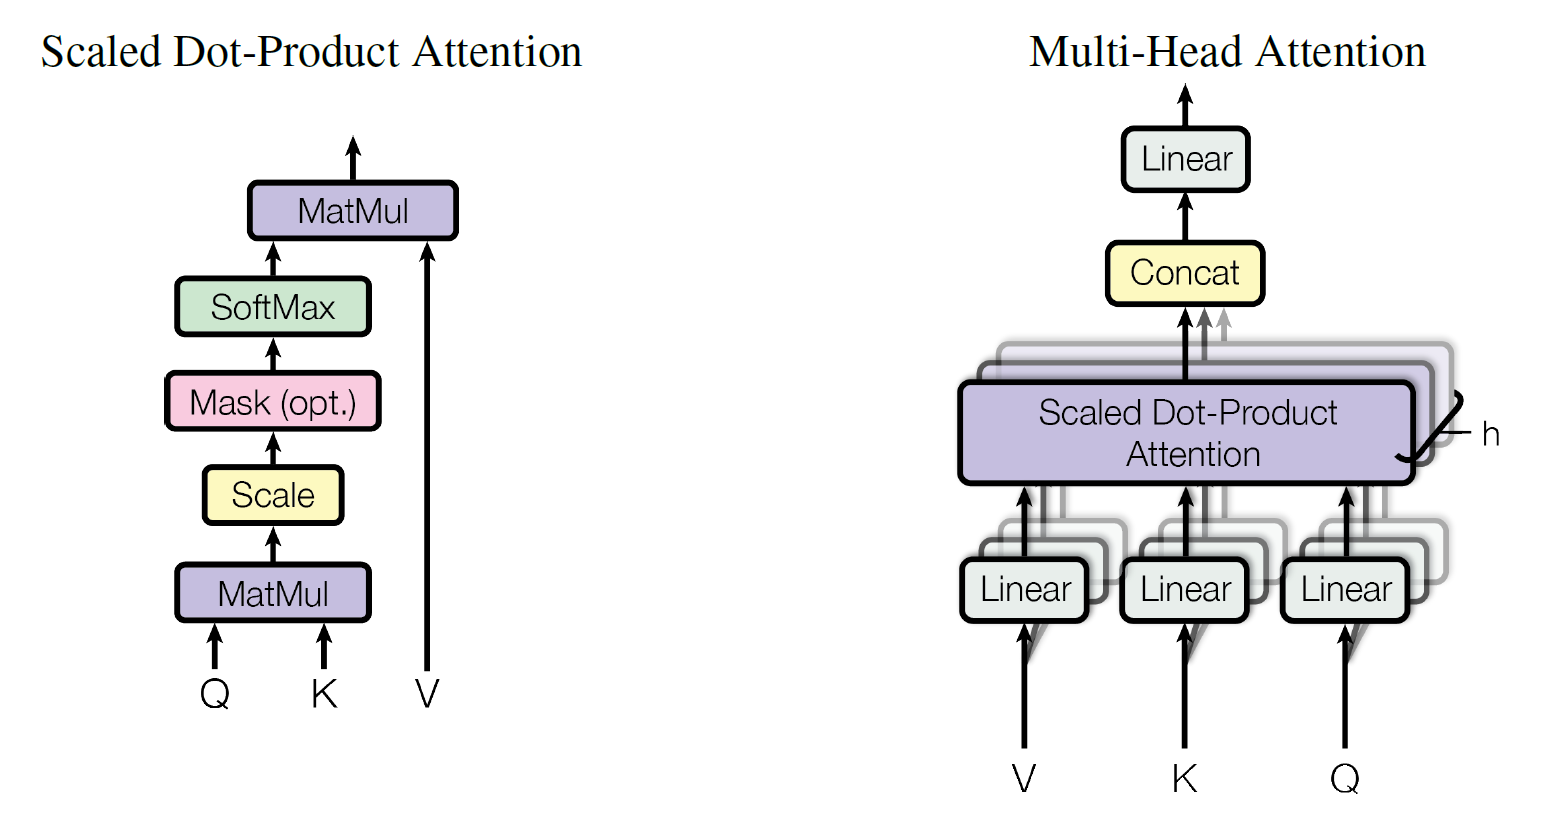
\includegraphics[keepaspectratio, width=120mm]{img/attentions-of-transformer.png}
	\caption{Transformerを構成するMulti-Head Attention(右)とそれを構成すScaled Dot-Product Attention(左)のモデルアーキテクチャ\protect\footnotemark[3]}
	\label{fig_attentions-of-transformer}
\end{figure}
\footnotetext[3]{\cite{vaswani_attention_nodate}より引用}

Scaled Dot-Product Attentionは式(\ref{scaled_dot_product_attention})で表される.
$Q$(Queue)は入力を意味し,式(\ref{scaled_dot_product_attention})は$Q$と$K$(Key)との類似度を基にした重みづけによって出力$V$(Value)を調節するような効果をもつ.

Multi-Head Attentionは式(\ref{multi_head_attention})で表される.
式(\ref{multi_head_attention})を構成する式\ref{scaled_dot_product_attention})の$Q,~ K,~ V$は同値であり,Transformerのデコーダへの入力文をOutput EmbeddingとPositional Encodingで加工したもの(Xとする)を表す.
これらの$Q,~ K,~ V$に$W_i^Q,~ W_i^K,~ W_i^V$を作用させて役割を変えている.
$QW_i^Q$はXのどの部分を処理するかを表し,$KW_i^K$はXの注目の仕方を表し,$VW_i^V$は出力の様子を調整する役割を担う.

\begin{align}
  \text { Attention }(Q, K, V) &= \operatorname{softmax}\left(\frac{Q K^{T}}{\sqrt{d_{k}}}\right) V
  \label{scaled_dot_product_attention}
  \\
  \text { MultiHead }(Q, K, V) &=\text { Concat }\left(\text { head }_{1}, \ldots, \text { head }_{\mathrm{h}}\right) W^{O}
  \label{multi_head_attention}
  \\
  \text { head }_{\mathrm{i}} &=\operatorname{Attention}\left(Q W_{i}^{Q}, K W_{i}^{K}, V W_{i}^{V}\right)
  \label{substituted_scaled_dot_product_attention}
\end{align}

% (教師なし分類にも触れる)
% @see p.549-

\subsection{BERT}
Liuらが2019年に提案したBERT(Bidirectional Encoder Representations from Transformers)は,文の意味や文脈を加味した自然言語処理を行うための機械学習モデルである\cite{aurellen20}\cite{devlin_bert_2019}.
研究者が大規模な計算資源を用いて自然言語の特徴を学習したBERTモデルを公開しており,学習されたモデルに用途に合わせた追加の学習を行うことで,小規模な計算資源で様々な自然言語タスクを高精度で行うことができる.
このような前段階での学習を事前学習,その後の用途に合わせた学習を転移学習と呼ぶ.

図\ref{fig_bert}に中間層が1つのBERTのモデルアーキテクチャを示す.
入力と出力はともに次元が等しいベクトルである.
中間層と出力層にはTransformerのエンコーダ部分が用いており,文から単語の意味を効果的に学習することができる.
また,個々のTransformerエンコーダが前の層の全てのノードから値を受け取っており,文を前から後ろに読む文脈情報と後ろから前に読む文脈情報の両方を加味した学習が可能である.
BERTモデルは,中間層の数や個々のTransformerの数,Transformer内のAttentionの数などを調整し,種々の自然言語処理タスクの性能を上げている.

\begin{figure}[H]
  \centering
  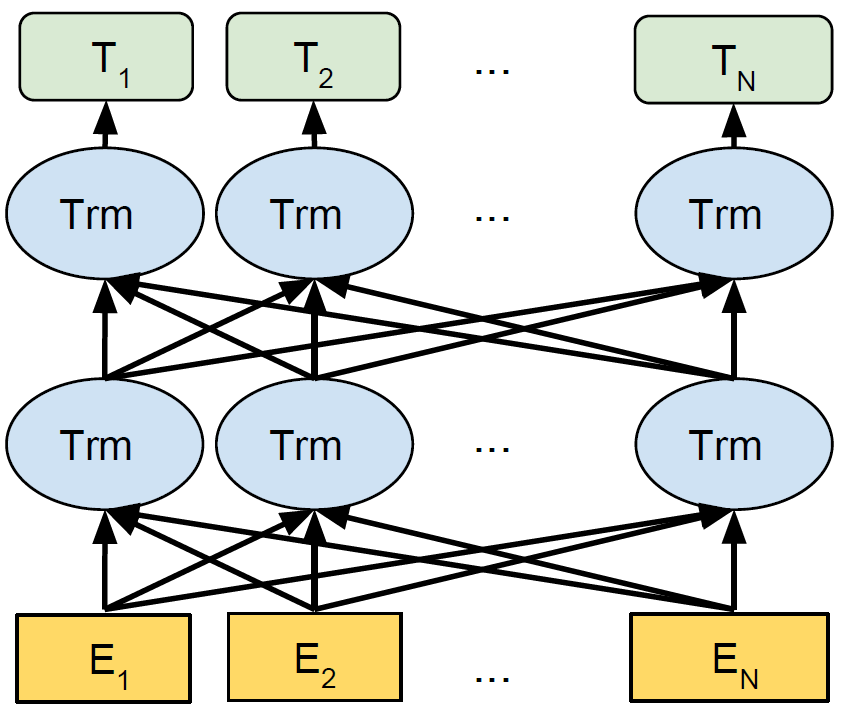
\includegraphics[keepaspectratio, width=80mm]{img/bert.png}
  \caption{中間層が1つのBERTのモデルアーキテクチャ\protect\footnotemark[4]
  \textcolor{red}{make width smaller}
  }
  \label{fig_bert}
\end{figure}
\footnotetext[4]{\cite{devlin_bert_2019}の図より一部抜粋}

図\ref{fig_fine_tuning_of_bert}にBERTの事前学習と転移学習の手順を示す.
事前学習で入力するベクトルの要素は,分類のための出力の次元調整に用いる定ベクトル[CLS],入力する2文の単語埋め込み,2文の分割位置を示す定ベクトル[SEP]で構成される.
図中の左の事前学習では,文法や単語の意味の意味を理解するためのMLM(Masked Language Model)としての学習と,文意と文脈を理解するためのNSP(Next Sentence Prediction)としての学習を同時に行う.

MLMとしての学習では,まずモデルに入力する2文の単語の15\%のうち,80\%を文字列[MASK]に置き換え,10\%を無作為に抽出した単語に置き換える.残りの10\%は何も置き換えない.
この置き換えにより,事前学習でしか入力しない文字列[MASK]について,事前学習と転移学習とのミスマッチを低減することができる.
その後,出力されたベクトルの入力でマスクされた位置と同じ位置の要素を使用し,マスク前の単語がどの単語であったかを予測する単語ごとの確率を計算して出力する.
% 1層の全結合層とソフトマックス関数
出力した確率とマスクした正解の単語を基に損失関数を計算し,モデルの重みの更新を行う.

NSPとしての学習では,入力文の50\%を文章中で連続する2文,残りの50\%を文章中で連続しない無作為に抽出された2文として入力する.
入力する2文には,文章中で連続した2文であるかそうでないかのラベル付けがなされている.
その後,出力されたベクトルの[CLS]と同じ位置の要素Cとラベルを使用してどちらの2文であったかの損失関数を計算し,モデルの重みを更新する.

\begin{figure}[H]
	\centering
	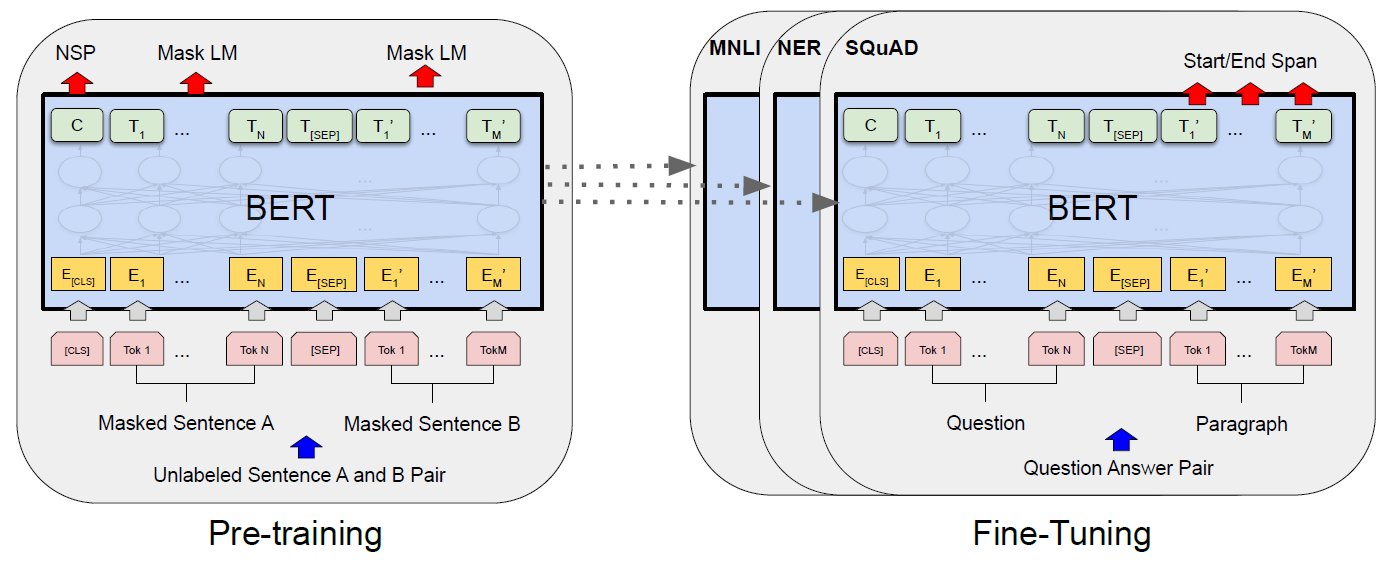
\includegraphics[keepaspectratio, width=120mm]{img/fine-tuning-of-bert.png}
	\caption{BERTの事前学習と転移学習の手順\protect\footnotemark[5]}
	\label{fig_fine_tuning_of_bert}
\end{figure}
\footnotetext[5]{\cite{devlin_bert_2019}より引用}

事前学習の後は,MNLI(Multi-Genre Natural Language Inference),NER(Named Entity Recognition),SQuAD(The Stanford Question Answering Dataset)などの行いたい自然言語処理タスクに合わせて入力と使用する出力の要素を変える.
図\ref{fig_single_sentence_classification_of_bert}に1文のクラス分類のためのBERTの転移学習のモデルアーキテクチャを示す.
この学習では文字列[CLS]と分類したい1文を入力し,[CLS]に対応する出力$\bm{C}$と正解のラベルを基に損失関数の計算を行っている.

% 交差エントロピー
% https://github.com/ThilinaRajapakse/simpletransformers/blob/master/docs/_docs/05-classification-models.md
% 実質ロジスティック回帰 p.150
% class RobertaClassificationHead(nn.Module):
%     """Head for sentence-level classification tasks."""
%     def __init__(self, config):
%         super().__init__()
%         self.dense = nn.Linear(config.hidden_size, config.hidden_size)
%         self.dropout = nn.Dropout(config.hidden_dropout_prob)
%         self.out_proj = nn.Linear(config.hidden_size, config.num_labels)

\begin{figure}[H]
	\centering
	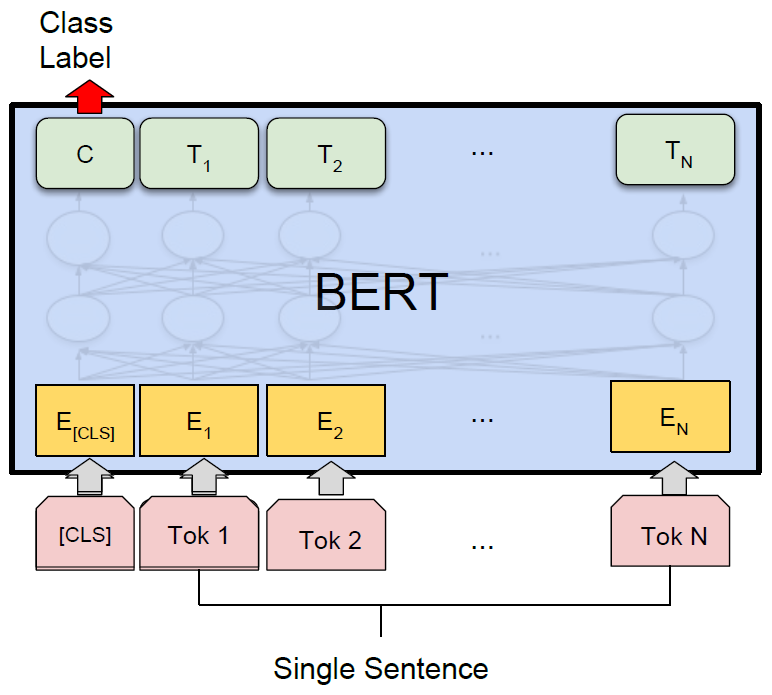
\includegraphics[keepaspectratio, width=120mm]{img/single-sentence-classification-of-bert.png}
	\caption{1文のクラス分類のためのBERTの転移学習\protect\footnotemark[6]}
	\label{fig_single_sentence_classification_of_bert}
\end{figure}
\footnotetext[6]{\cite{devlin_bert_2019}より引用}


% 転移学習 325 345-348 475-477

% @see https://www.youtube.com/watch?v=IaTCGRL41_k&list=PLhDAH9aTfnxL4XdCRjUCC0_flR00A6tJR&index=17
% @see https://data-analytics.fun/2020/05/02/understanding-bert/
% @see https://qiita.com/omiita/items/72998858efc19a368e50

\subsection{RoBERTa}
Devlinらが2019年に提案したRoBERTaはBERTの学習方法を改善した機械学習モデルで,多くの自然言語処理タスクのベンチマークでBERTのスコアを上回る.
RoBERTaのモデルアーキテクチャは図\ref{fig_bert}のBERTと同じものを使用する.
MLMとしての学習でBERTでは10回学習するごとに同じマスクを使用していたため,どの学習でも異なるマスクを使用することでSQuAD(Stanford Question Answering Dataset)とSST-2(The Stanford Sentiment Treebank)のスコアを向上させた.
% 余裕があれば表を挿入
BERTが行っていたNSPとしての学習は比較実験により有効でないことが確認され,RoBERTaではこれを行っていない.
比較実験では,BERTが行ったSEGMENT-PAIRのNSPの学習の代わりにSENTENCE-PAIRのNSPの学習,FULL-SENTENCESのNSPをしない学習,DOC-SENTENCESのNSPをしない学習を行い,NSPの学習を行わなくてもSQuAD,SST-2,MNLI-m(The Multi-Genre Natural Language Inference Matched),RACE(Reading Comprehension)のスコアが概ね向上することを確認した.
% 余裕があれば表を挿入
BERTでは学習データとして250万単語のEnglish Wikipediaと80万単語のBooksCorpusで計16GBのデータを用いていたが,RoBERTaではこれに加えて76GBのCC-News,38GBのOpenWebText,31GBのStoriesを学習した.
さらに,1回の学習で用いるデータサイズ(バッチサイズ)を256から8,000に増やすことで,BERTよりもSQuAD,MNLI-m,SST-2のスコアが向上することを確認した.


表\ref{roberta_glue}にBERTとRoBERTaのGLUE(General Language Understanding Evaluation)タスクのベンチマークスコアを示す.
それぞれのベンチマークでは以下のタスクを行っている.

\begin{itemize}
  \item MNLI(The Multi-Genre Natural Language Inference)
  \begin{itemize}
    \item 2つの文が含意,矛盾,中立のどの関係にあるかを判定
  \end{itemize}
  \item QNLI(Question Natural Language Inference)
  \begin{itemize}
    \item 質問文とともに入力した文が質問に対する正しい回答であるかを判定
  \end{itemize}
  \item QQP(Quora Question Pairs)
  \begin{itemize}
    \item 2つの質問文が同じ意味であるかを判定
  \end{itemize}
  \item RTE(Recognizing Textual Entailment)
  \begin{itemize}
    \item 2つの文が含意関係にあるかを判定
  \end{itemize}
  \item SST(The Stanford Sentiment Treebank)
  \begin{itemize}
    \item 映画のレビュー文がポジティブであるかネガティブであるかを判定
  \end{itemize}
  \item MRPC(Microsoft Research Paraphrase Corpus)
  \begin{itemize}
    \item 2つの文が同じ意味であるかを判定
  \end{itemize}
  \item CoLA(The Corpus of Linguistic Acceptability)
  \begin{itemize}
    \item 英文の文法が正しいかを判定
  \end{itemize}
  \item STS(Semantic Textual Similarity Benchmark)
  \begin{itemize}
    \item ニュースの2つの見出し文の類似度を5段階で評価
  \end{itemize}
\end{itemize}
本研究におけるクラス分類ではSTSのスコアが重要であり,このスコアはRoBERTaの学習方法により90.0から92.4に向上している.

\begin{table}[H]
  \caption{
    BERTとRoBERTaのGLUEタスクのベンチマークスコア.
    \protect\footnotemark[7]
    全ての結果は24層のアーキテクチャを使用し,5回の実行結果の中央値を取っている.
    }
  \centering
  \vspace{3.0mm}
  % {\tabcolsep=0.13cm
    % \begin{tabular}{lccccccccc}
    % \hline
    % & \textbf{MNLI} & \textbf{QNLI} & \textbf{QQP} & \textbf{RTE} & \textbf{SST} & \textbf{MRPC} & \textbf{CoLA} & \textbf{STS} & \textbf{WNLI} \\
    % \hline
    % $\text{BERT}_{\text{LARGE}}$ & 86.6 & 92.3 & 91.3 & 70.4 & 93.2 & 88.0 & 60.6 & 90.0 & - \\
    % RoBERTa & \textbf{90.2} & \textbf{94.7} & \textbf{92.2} & \textbf{86.6} & \textbf{96.4} & \textbf{90.9} & \textbf{68.0} & \textbf{92.4} & 91.3 \\
    \begin{tabular}{lcccccccc}
    \hline
    & \textbf{MNLI} & \textbf{QNLI} & \textbf{QQP} & \textbf{RTE} & \textbf{SST} & \textbf{MRPC} & \textbf{CoLA} & \textbf{STS} \\
    \hline
    $\text{BERT}_{\text{LARGE}}$ & 86.6 & 92.3 & 91.3 & 70.4 & 93.2 & 88.0 & 60.6 & 90.0 \\
    RoBERTa & \textbf{90.2} & \textbf{94.7} & \textbf{92.2} & \textbf{86.6} & \textbf{96.4} & \textbf{90.9} & \textbf{68.0} & \textbf{92.4} \\
    \hline
  \end{tabular}
  % }
  \label{roberta_glue}
\end{table}
\footnotetext[7]{\cite{liu_roberta_2019}より一部抜粋}

% @see https://note.com/npaka/n/n5086fc19c5fc

% @see https://data-analytics.fun/2020/05/08/understanding-roberta/
% @see https://github.com/pytorch/fairseq/tree/main/examples/roberta
% @see https://tensorflow.classcat.com/2021/05/16/huggingface-transformers-4-6-pretrained-models/
% @see https://www.youtube.com/watch?v=T7nbrIJtYlE&list=PLhDAH9aTfnxL4XdCRjUCC0_flR00A6tJR&index=22
% @see 

%%%%%%%%%%%%%%%%%%%%%%%%%%%%%%

\section{教師あり学習の評価}
教師あり学習は,訓練データ(教師データ)と呼ばれる特徴を学習したデータとは別に,学習に用いていないテストデータと呼ばれるデータで入出力の評価を行う必要がある\cite{aurellen20}.
この評価は,モデルに未知のデータを入力したときに目的の出力を得るために必要な操作である.

訓練データで目的の出力を得られてもテストデータで目的の出力が得られないとき,モデルは過学習(過剰適合)しているといい,モデルは未知のデータに対応できていない.
過学習は,モデルの学習回数が多く訓練データの特徴を学習しすぎたときや,学習の手法が適切でないときに起こり得る.
一方で,訓練データでも目的の出力を得られていないとき,モデルは過少適合しているという.
過少適合はモデルの学習回数が少なく訓練データの特徴を学習できていないときや,学習の手法が適切でないときに起こり得る.
目的の出力が得られているかどうかは,学習ごとの損失関数の出力の大きさから確認することができる.

同じデータでテストデータの評価を行いたいときは,データを訓練データとテストデータに分割して評価する.
例えば,100件のデータの80件を訓練データとして学習し,学習に用いていない20件のデータをテストデータとして評価を行う.
% 交差検証の可能性を残す

% @see 

\subsection{混同行列を用いた分類器の評価}
分類器の評価では,混同行列を用いたいくつかの評価指標がよく用いられる\cite{aurellen20}.
混同行列は,分類器の入力の$n$種類のラベルと出力の$n$種類のラベルの計$n^2$組の組み合わせについて,それぞれの数を要素とした$n$次正方行列である.

\textcolor{red}{add \textbackslash newpage}
\newpage

表\ref{confusion_matrix}に10件のデータを0か1かの2値ラベルで分類したときの混同行列の例を示す.
評価指標の計算で着目するクラスを陽性クラス(positive class),その他のクラスを陰性クラス(negative class)といい,表\ref{confusion_matrix}では1を陽性クラス,0を陰性クラスとして考える.
表\ref{confusion_matrix}の2件のデータは正しく分類した陰性クラスであり,真陰性(TN; true negative)があるという.
表\ref{confusion_matrix}の1件のデータは誤って陽性クラスだと分類した陰性クラスであり,偽陽性(FP; false positive)があるという.
表\ref{confusion_matrix}の3件のデータは誤って陰性クラスだと分類した陽性クラスであり,偽陰性(FN; false negative)があるという.
表\ref{confusion_matrix}の4件のデータは正しく分類した陽性クラスであり,真陽性(TP; true positive)があるという.
以降の小小節
\ref{subsubsection_precision},
\ref{subsubsection_recall},
\ref{subsubsection_mcc},
では,これらTN,FN,FP,TPを用いて計算した評価指標である適合率,再現率,マシューズ相関係数について記す.

\begin{table}[H]
  \caption{
    混同行列の例
    }
  \vspace{3mm}
  \centering
    \begin{tabular}{c|cc}
     & 予測は0 & 予測は1 \\
    \hline
    入力は0 & 2 & 1 \\
    入力は1 & 3 & 4
  \end{tabular}
  % }
  \label{confusion_matrix}
\end{table}

% @see 92-94 104-106
% @see https://zellij.hatenablog.com/entry/20120214/p1
% @see https://www.datarobot.com/jp/blog/matthews-correlation-coefficient/


\subsubsection{適合率}
\label{subsubsection_precision}
適合率(precision)は,陽性クラスだと分類したデータのうち真陽性クラスであるデータの割合である\cite{aurellen20}.
表\ref{confusion_matrix}の例では,ラベルが1だと予測データのうち実際に1であったデータの割合を指す.
したがって,式(\ref{precision})のように適合率が計算される.

\begin{align}
  precision ~=~ \frac{TP}{TP+FP} ~=~ \frac{4}{4+1} ~=~ 0.8
  \label{precision}
\end{align}

\textcolor{red}{add \textbackslash newpage}
\newpage

適合率は,数ある映像から子どもに観せても安心な映像を検出する分類器などで重視される.
観せて安心な映像を陽性クラスの映像だとしたとき,分類器の適合率が高ければ,観せて安心な映像だと分類した映像の多くは真に観せて安心な映像であることが多い.


\subsubsection{再現率}
\label{subsubsection_recall}
再現率(recall)は,陽性クラスのデータのうち真陽性クラスであるデータの割合である\cite{aurellen20}.
表\ref{confusion_matrix}の例では,ラベルが1のデータのうち予測も1であったデータの割合を指す.
したがって,式(\ref{recall})のように再現率が計算される.

\begin{align}
  recall ~=~ \frac{TP}{TP+FN} ~=~ \frac{4}{4+3} ~\sim~ 0.57
  \label{recall}
\end{align}

再現率は,監視カメラに映る人物の映像から万引き犯の映像を検出する分類器などで重視される.
万引き犯の映像を陽性クラスの映像だとしたとき,分類器の再現率が高ければ,万引き犯の映像の多くは予測も万引き犯の映像となる.

適合率と再現率は一般にトレードオフの関係にあり,分類器の目的によってそれぞれの評価指標をどれほど重要視するかを考慮する必要がある.
上述の監視カメラの例では,適合率が低く万引き犯だと分類した映像のいくつかが万引き反でない人物となってしまうことよりも,再現率が高く確実に万引き犯を検出できることの方が重要である.

\textcolor{red}{add \textbackslash newpage}
\newpage

\subsubsection{マシューズ相関係数}
\label{subsubsection_mcc}
Matthewsが1975年に提案したマシューズ相関係数(MCC;Matthews Correlation Coefficient)は,混同行列を基に分類器の精度を総合的に評価する指標で,TP,TN,FP,FNの数が不均衡なときにも頑健に評価できる\cite{chicco_advantages_2020}.
マシューズ相関係数は式(\ref{mcc})のように計算される$[-1, 1]$の範囲の実数値であり,この値が大きいほど分類器の精度が高いといえる.
\begin{align}
  MCC ~=~ \frac{\mathrm{TP} \times \mathrm{TN}-\mathrm{FP} \times \mathrm{FN}}{\sqrt{(\mathrm{TP}+\mathrm{FP}) \times(\mathrm{TP}+\mathrm{FN}) \times(\mathrm{TN}+\mathrm{FP}) \times(\mathrm{TN}+\mathrm{FN})}}
  \label{mcc}
\end{align}

% (1*1-0*0)/(1*1*1*1)^-1 = 1
% (0*0-1*1)/(1*1*1*1)^-1 = -1
% @see https://www.datarobot.com/jp/blog/matthews-correlation-coefficient/

\section{文章の距離の算出}
\label{section_sentence_distance}
後述のクラスタリングを行うにあたり,クラスタリングに必要な文章の距離(非類似度)の算出法について記す.
本節\ref{section_sentence_distance}では,小節\ref{subsection_sentence_bert}で文章を埋め込みに変換するSentence-BERTについて説明し,小節\ref{subsection_cosine_distance}で変換した埋め込みを用いて計算するコサイン距離について説明する.

\textcolor{red}{add \textbackslash newpage}
\newpage

\subsection{Sentence-BERT}
\label{subsection_sentence_bert}
Reimersらが2019年に提案したSentence-BERTは,文の意味や文脈を加味した文埋め込みを生成するためのBERTを転移学習した機械学習モデルである\cite{reimers_sentence-bert_2019}.
図\ref{fig_sentence_bert}にSentence-BERTのモデルアーキテクチャを示す.
Sentence-BERTでは転移学習済みのBERTに1つの文を入力し,出力したベクトル群にpoolingと呼ばれる情報の抽出処理を行って文章の埋め込みを得る.
転移学習では,埋め込みを応用したSTSタスクなどの精度を上げるために,
% 3つ関数Classification Objective Function,Regressioon Objective Function,Triplet Objective Functionを用いた
3種類の工夫された学習が行われている.
poolingでは3つの手法が比較されており,BERTで出力したベクトル群の平均を埋め込みとする手法が最もSTSタスクのスコアが優れていた.

% @see 3. Model


\begin{figure}[H]
	\centering
	% 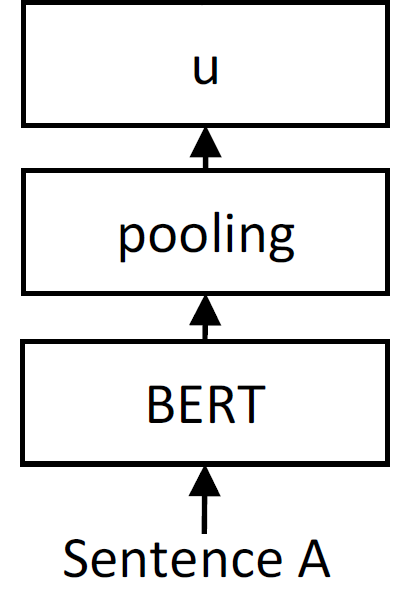
\includegraphics[keepaspectratio, width=120mm]{img/sentence-bert.png}
	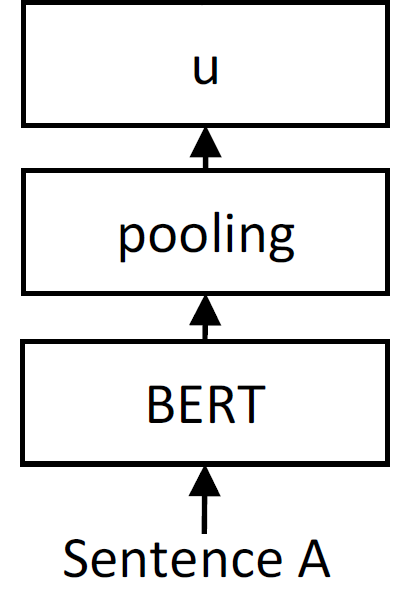
\includegraphics[keepaspectratio, width=60mm]{img/sentence-bert.png}
	\caption{Sentence-BERTのモデルアーキテクチャ\protect\footnotemark[8]}
	\label{fig_sentence_bert}
\end{figure}
\footnotetext[8]{\cite{reimers_sentence-bert_2019}の図より一部抜粋}

\textcolor{red}{add \textbackslash newpage}
\newpage

BERTやRoBERTaで1万文から最も意味的類似度が高い2文を得たいとき,図\ref{fig_fine_tuning_of_bert}のように2文同時に入力すると$\frac{10000(10000-1)}{2}=49995000$回の実行が必要であり,Reimersらの実験では65時間の処理を要した.
そこでReimersらは,BERTやRoBERTaに1文を入力して単語埋め込みを得る処理を$10000$回行い,埋め込み間の類似度を計算し,処理時間を約5秒に短縮した.
埋め込み間の類似度には,式(\ref{cosine_similarity})に示すコサイン類似度が用いられている.

\begin{align}
  \text{cos-sim}\left(\bm{u}, \bm{v}\right) = \frac{\bm{u} \cdot \bm{v}}{\|\bm{u}\|\|\bm{v}\|}
  \label{cosine_similarity}
\end{align}

表\ref{sentence_bert_evaluation}にSentEvalツールキットを用いた文埋め込みの比較評価を示す.
表より,Sentence-BERTは多くの自然言語処理タスクにおいて2019年の最先端のスコアを有することがわかる.

\begin{table}[H]
  \caption{
    SentEvalツールキットを用いた文埋め込みの比較評価
    \protect\footnotemark[9]
    }
  \vspace{3mm}
  \centering
  {\tabcolsep=0.1cm
    \begin{tabular}{l|cccccccc}
      \hline Model & MR & CR & SUBJ & MPQA & SST & TREC & MRPC & Avg. \\
      \hline Avg. GloVe embeddings & $77.25$ & $78.30$ & $91.17$ & $87.85$ & $80.18$ & $83.0$ & $72.87$ & $81.52$ \\
      Avg. fast-text embeddings & $77.96$ & $79.23$ & $91.68$ & $87.81$ & $82.15$ & $83.6$ & $74.49$ & $82.42$ \\
      Avg. BERT embeddings & $78.66$ & $86.25$ & $94.37$ & $88.66$ & $84.40$ & $92.8$ & $69.45$ & $84.94$ \\
      BERT CLS-vector & $78.68$ & $84.85$ & $94.21$ & $88.23$ & $84.13$ & $91.4$ & $71.13$ & $84.66$ \\
      InferSent - GloVe & $81.57$ & $86.54$ & $92.50$ & $\mathbf{9 0 . 3 8}$ & $84.18$ & $88.2$ & $75.77$ & $85.59$ \\
      Universal Sentence Encoder & $80.09$ & $85.19$ & $93.98$ & $86.70$ & $86.38$ & $\mathbf{9 3 . 2}$ & $70.14$ & $85.10$ \\
      \hline SBERT-NLI-base & $83.64$ & $89.43$ & $94.39$ & $89.86$ & $88.96$ & $89.6$ & $\mathbf{7 6 . 0 0}$ & $87.41$ \\
      SBERT-NLI-large & $\mathbf{8 4 . 8 8}$ & $\mathbf{9 0 . 0 7}$ & $\mathbf{9 4 . 5 2}$ & $90.33$ & $\mathbf{9 0 . 6 6}$ & $87.4$ & $75.94$ & $\mathbf{8 7 . 6 9}$ \\
      \hline
    \end{tabular}
  }  
  \label{sentence_bert_evaluation}
\end{table}
\footnotetext[9]{\cite{reimers_sentence-bert_2019}より引用}

% 文章間の意味的類似度の算出を約5秒に短縮し,STSタスクで2019年の最先端のスコアを有している.
% SentenceTransformer(
%   (0): Transformer({'max_seq_length': 128, 'do_lower_case': False}) with Transformer model: BertModel 
%   (1): Pooling({'word_embedding_dimension': 384, 'pooling_mode_cls_token': False, 'pooling_mode_mean_tokens': True, 'pooling_mode_max_tokens': False, 'pooling_mode_mean_sqrt_len_tokens': False})
% )
% @see https://data-analytics.fun/2020/08/04/understanding-sentence-bert/
% @see https://www.vareal.co.jp/column/sentence-bert%E8%AB%96%E6%96%87-%E5%92%8C%E8%A8%B3/
% @see https://github.com/UKPLab/sentence-transformers
% @see https://www.google.com/search?client=firefox-b-d&q=paraphrase-MiniLM-L6-v2


\subsection{コサイン距離}
\label{subsection_cosine_distance}
\textcolor{red}{
式(\ref{cosine_distance})にコサイン距離は,2つのベクトルの距離の指標の1つである.
2つの3次元ベクトル間のコサイン距離は,2つのベクトルがなす角の大きさに相当する.
}
コサイン距離は,単語埋め込みや文章の埋め込みの距離の算出によく用いられる.

\begin{align}
  \text{cos-dist}\left(\bm{u}, \bm{v}\right) ~&=~
  1 -
  \text{cos-sim}\left(\bm{u}, \bm{v}\right) ~=~
  1 - \frac{\bm{u} \cdot \bm{v}}{\|\bm{u}\|\|\bm{v}\|}
  \label{cosine_distance}
\end{align}

%%%%%%%%%%%%%%%%%%%%%%%%%%%%%%
\section{階層的クラスタリング}
\label{section_clustering}
クラスタリングは,データの集合を何らかのアルゴリズムに基づいてクラスタと呼ばれる部分集合に分割する教師なし学習である
% \cite{aurellen20}
.
類似したデータをクラスタにまとめることで,データの要約や傾向の分析を行うことができる.

本節\ref{section_clustering}では,小節\ref{subsection_wards_method}でクラスタ間の距離を算出するWard法について説明し,小節\ref{subsection_hierarchical_clustering}でクラスタリングの一種である階層的クラスタリングについて説明する.
% し,小節\ref{subsection_dendrogram}で階層的クラスタリングの工程を可視化するデンドログラムについて説明する.

% @see 木村先生のデータ解析法
% @see 神嶌先生の講義資料

% \subsection{非階層クラスタリング}
% ~
% @see p.12

\subsection{Ward法}
\label{subsection_wards_method}
階層的クラスタリングの処理には,データの部分集合であるクラスタ同士の距離(クラスタ間距離)が必要となる.
クラスタ間距離の算出には単一連結法や最遠隣法など様々な手法が用いられているが,本研究では1963年にWardが提案したWard法(最小分散法)を使用する\cite{murtagh_wards_2014}.
Ward法は異常なデータの値(外れ値)の影響を受けにくく,クラスタ間距離の算出法として広く用いられている.

\textcolor{red}{add \textbackslash newpage}
\newpage

Ward法では式(\ref{wards_method})に示すように,
併合後のクラスタ$C_{k} \cup C_{c}$の分散と
併合前のクラスタ$C_{k}, C_{c}$のそれぞれの分散の和との差$d_{k c}$をクラスタ間距離とする.

% 分散の実装方法にはユークリッド距離の観点から実装したものと平方ユークリッド距離の観点から実装したものがあるが,本研究ではデンドログラムでの分析で有用なユークリッド距離の観点から実装したものを用いる.
% ユークリッド距離を使うか平方ユークリッド距離を使うかの実装の差がある

\begin{align}
  d_{k c} &= \operatorname{Var} \left( C_{k} \cup C_{c} \right)
  -
  \left(
    \operatorname{Var}\left(C_{k}\right)
    +
    \operatorname{Var}\left(C_{c}\right)
  \right)
  \label{wards_method}
\end{align}

% @see https://docs.scipy.org/doc/scipy/reference/generated/scipy.cluster.hierarchy.linkage.html


\subsection{階層的クラスタリング}
\label{subsection_hierarchical_clustering}
階層的クラスタリング(凝集型クラスタリング)は,図\ref{fig_clustering_example}に示すようにクラスタ間距離が最も近い2つのクラスタを順次1つのクラスタに結合していく手法である.
\textcolor{red}{
図\ref{fig_clustering_example}の右側のグラフのように,階層的クラスタリングの様子をツリー状に可視化したものをデンドログラムという.
}

結合前のクラスタは結合後のクラスタの部分集合となり,最終的には1つのクラスタとなる.
従って階層的クラスタリングは,このような部分集合の階層構造をもつデータの分析に有用である.
どのクラスタ間距離でクラスタの結合を止めるかによって,様々な粒度のクラスタ群を得ることができる.

\begin{figure}[H]
	\centering
	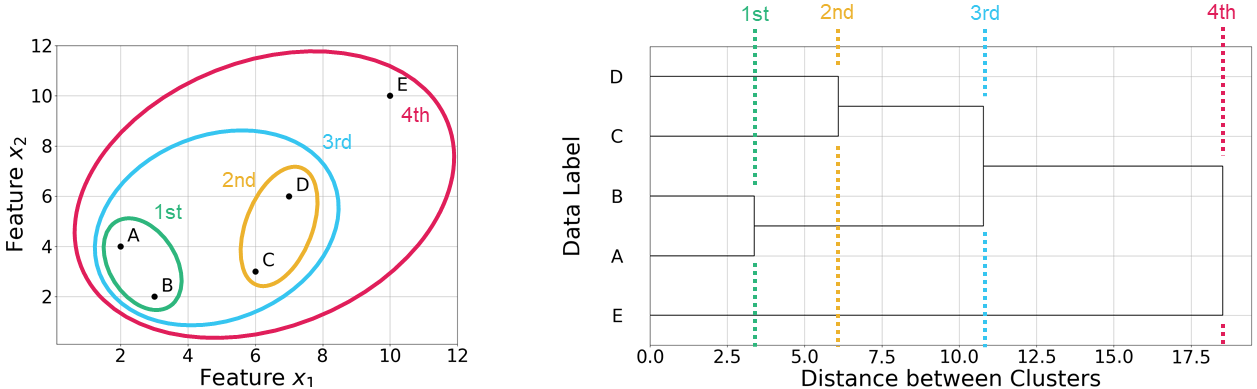
\includegraphics[keepaspectratio, width=120mm]{img/clustering_example.png}
	\caption{階層的クラスタリング}
	\label{fig_clustering_example}
\end{figure}

% @see p.261

% \subsection{デンドログラム}
% \label{subsection_dendrogram}


% \subsection{(その他使用した手法)}
% ~
% % @see 

% \subsection{t-SNE (使うかも)}
% ~
% % @see 

\textcolor{red}{add \textbackslash newpage}
\newpage

\subsection{\textcolor{red}{シルエット係数}}
式(\ref{silhouette_coefficient})に示すシルエット係数は,階層的クラスタリングの評価指標のひとつである\cite{aranganayagi_clustering_2007}.
全データのシルエット係数の平均$\overline{Sil(i)}$が大きいほど同一クラスタ内のデータがより類似し,異なるクラスタ間のデータがより類似していないといえる.

\begin{align}
  Sil(i) &= \frac{b(i) - a(i)}{\max ( b(i) , a(i))}
  \label{silhouette_coefficient}
  \\
  a(i)
  &=\frac{1}{\left|C_{\text {in}}\right|-1} \sum_{\boldsymbol{x}_{j} \in C_{\text {in }}}\left\|\boldsymbol{x}_{i}-\boldsymbol{x}_{j}\right\|
  \quad(x_i \in C_{in} ,~ i \neq j)
  \label{a_i}
  \\
  b(i)
  &=\frac{1}{\left|C_{\text {near }}\right|} \sum_{\boldsymbol{x}_{k} \in C_{\text {near }}}\left\|\boldsymbol{x}_{i}-\boldsymbol{x}_{k}\right\|
  = \min_C{\left( D(i, C) \right)}
  \label{b_i}
  \\
  D(i, C)
  &=\frac{1}{\left|C \right|} \sum_{\boldsymbol{x}_{h} \in C}\left\|\boldsymbol{x}_{i}-\boldsymbol{x}_{h}\right\|
  \quad (x_i \in C_{in},~ C \cap C_{in} = \emptyset)
  \label{d_ic}
\end{align}

式(\ref{a_i})に示す$a(i)$はデータ$\bm{x}_i$と$\bm{x}_i$が属するクラスタ$C_{in}$内の他の全データ$\bm{x}_j \in C_{in}$との距離の平均である.
$a(i)$が0に近いほどクラスタ$C_{in}$内のデータがよく類似しているといえる.

式(\ref{b_i})に示す$b(i)$はデータ$\bm{x}_i$と$\bm{x}_i$の最近傍のクラスタ$C_{near}$内の他の全データ$\bm{x}_k \in C_{near}$との距離の平均である.
具体的には,$D(i, C)$をクラスタ$C_{in}$以外のあるクラスタ$C$についてデータ$x_i$とクラスタ$C$内の全データ$\bm{x}_h \in C$との距離の平均だとしたとき,$b(i)$は任意のCにおける$D(i, C)$の最小値として計算される.
$b(i)$が1に近いほど異なるクラスタのデータが類似していないといえる.

% $a(i)$,$b(i)$から計算されるシルエット係数$Sil(i)$は$[-1, 1]$の範囲の値であり,1に近いほどよく凝集と乖離をしているといえる.
% 一方で,$Sil(i)$が0に近いデータが多いと複数の凝集したデータ群が1つのクラスタに属することがある.
% また,$Sil(i)$が$-1$に近いデータが多いと異なるクラスタのデータが特徴空間内で重なってしまうことが多く,クラスタの所属判定が誤っている可能性が高い.

% 本当は平均だけでなくデータごとのシルエット係数を図示するべきだった

% % @see https://hkawabata.github.io/technical-note/note/ML/Evaluation/silhouette-analysis.html

\textcolor{red}{add \textbackslash newpage}
\newpage

\section{k-NN分類法}
k-NN分類法(k近傍法)は,クラスが既知のデータ群が存在するときに新規に入力したデータのクラスを推定するためのクラス分類手法である\cite{aurellen20}.
新規のデータが入力されたとき,そのデータとの距離が最も近い既存のデータを順にk個選択し,k個のデータのクラスのうち最も多かったクラスを新規のデータのクラスと推定する.
kは事前に設定しておく必要がある.
% 距離の定義
% 教師あり学習

% % @see p.11,24

%%%%%%%%%%%%%%%%%%%%%%%%%%%%%%%%%%%%%%%%%%%%%%%%%%%%%%%%%%%%
\chapter{関連研究}
%%%%%%%%%%%%%%%%%%%%%%%%%%%%%%%%%%%%%%%%%%%%%%%%%%%%%%%%%%%%
\label{chapter_related_studies}


%%%%%%%%%%%%%%%%%%%%%%%%%%%%%%
\section{\textcolor{red}{BERTが事前学習した自然言語の特徴を用いてニュース推薦を行う研究}}

% @see 

% \subsection{トピックマップ}
% ~
% @see 

\subsection{UNBERT: User-News Matching BERT for News Recommendation}
Zhangらは,日々追加される新しい記事から読者の関心度が高い記事を推薦するため,BERTを用いたニュース推薦手法を提案した\cite{zhang_unbert_2021}.
LSTUR,FIM,NAML,NRMS,NPA,DKNなどのニューラルネットワークを用いた既存のニュース推薦手法は,学習していない特徴を持つ新しい記事が入力されたときに類似した記事を推薦できない問題をもつ.
この問題はコールドスタート問題と呼ばれ,ニュース推薦システムの大きな課題となっている.

そこでZhangらは,豊富な言語知識を事前学習したBERTモデルを利用し,コールドスタート問題に強いニュース推薦のための機械学習モデルとして,図\ref{fig_unbert_inputs},\ref{fig_unbert_model_architecture}に示すUNBERTを提案した.
Zhangらの実験では,学習済みの古い記事と未学習の新しい記事が読者が連続して読んだものであるかを分類し,既存手法と分類性能を比較した.
実験の結果,図\ref{fig_unbert_evaluation}に示すようにUNBERTが先に述べたどの既存手法よりも優れた性能で分類を行うことができた.
% 本当はAUC(適合率と再現率を考慮している)
% 評価が切り抜かれているのでかなり怪しい

\begin{figure}[H]
	\centering
	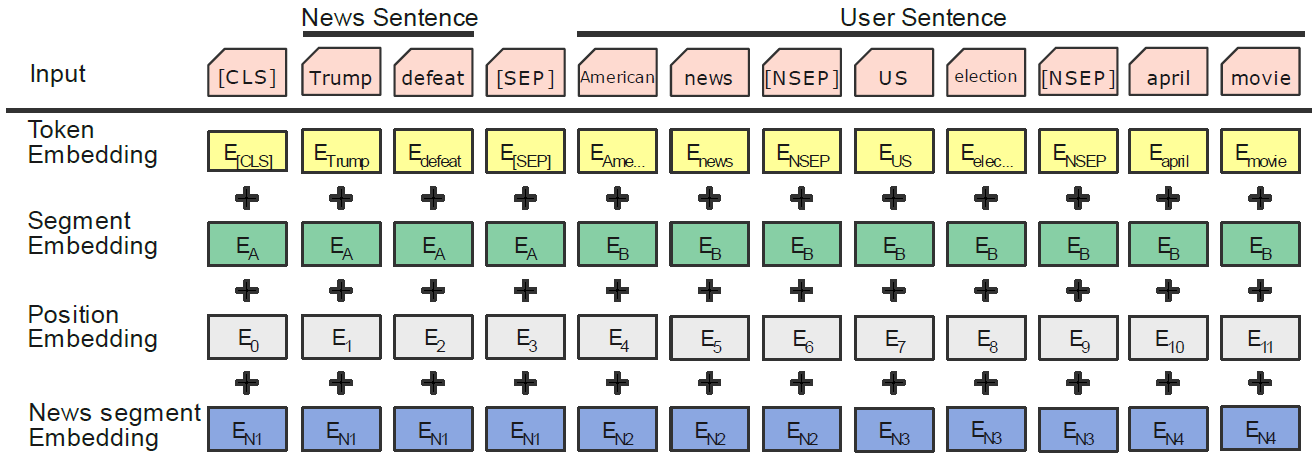
\includegraphics[keepaspectratio, width=120mm]{img/unbert_inputs.png}
	\caption{
    UNBERTの入力.
    \protect\footnotemark[10]
    新規の記事の文と読者が閲覧した複数の記事の文を文字列[CLS],[SEP],[NSEP]で分割して入力する.
  }
	\label{fig_unbert_inputs}
\end{figure}
\footnotetext[10]{\cite{zhang_unbert_2021}より引用}

\begin{figure}[H]
	\centering
	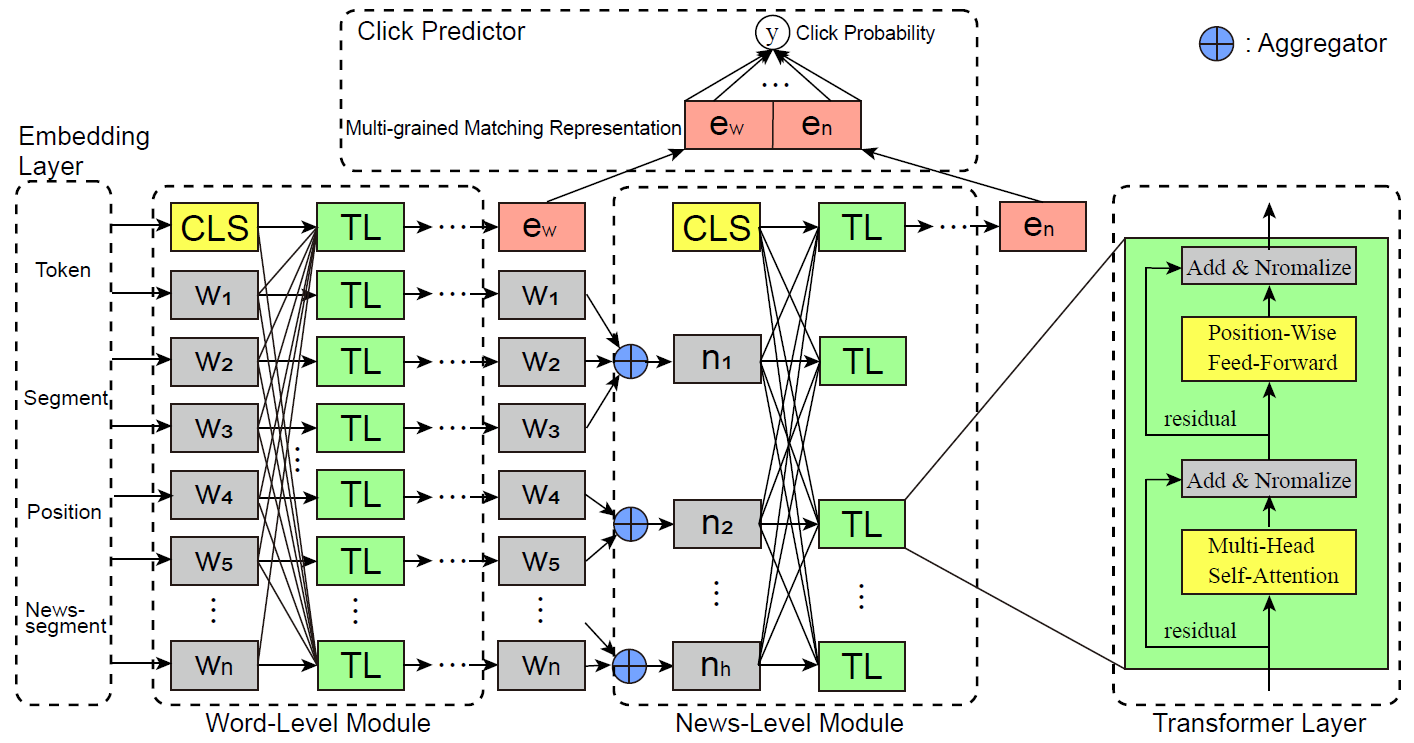
\includegraphics[keepaspectratio, width=120mm]{img/unbert_model_architecture.png}
	\caption{
    UNBERTのモデルアーキテクチャ.
    \protect\footnotemark[11]
    単語レベルの特徴の学習と文全体の特徴の学習で2つのBERTモデルを使用している.
    また,文字列[CLS]に対応する位置の出力を使用し,入力した2種類の記事が連続して読まれたものであるか確率を予測する.
  }
	\label{fig_unbert_model_architecture}
\end{figure}
\footnotetext[11]{\cite{zhang_unbert_2021}より引用}

\begin{figure}[H]
	\centering
	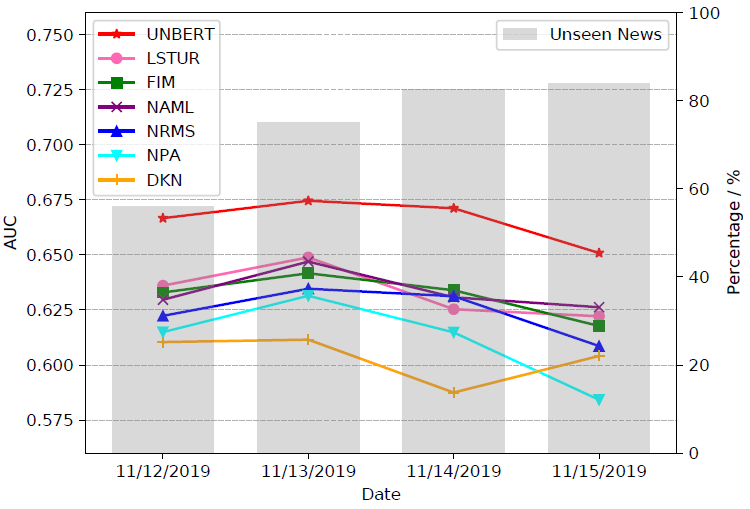
\includegraphics[keepaspectratio, width=120mm]{img/unbert_evaluation.png}
	\caption{
    各手法の新しい記事の分類性能.
    \protect\footnotemark[12]
    学習と分類のためのデータセットにはMIND(Microsoft News Dataset)を使用した.
    各手法のモデルは2019年11月19日から2019年11月11日の記事を学習している.
    分類性能の評価指標には分類の適合率と再現率を用いたAUCと呼ばれる評価指標を使用した.
  }
	\label{fig_unbert_evaluation}
\end{figure}
\footnotetext[12]{\cite{zhang_unbert_2021}より引用}


Zhangらの研究から,BERTが事前学習した自然言語の特徴が記事を入力とするタスクに応用可能であることがわかる.
本研究では,この自然言語の特徴を記事の文の分類タスクと文埋め込みを生成するタスクに応用する.

% @see 

% \subsubsection{(LDAの利用)}
% ~
% @see 

%%%%%%%%%%
% \section{LSI}
% ~
% @see 


%%%%%%%%%%%%%%%%%%%%%%%%%%%%%%
\section{ニュース推薦システムのバイアスを解決する研究}
% ~
% @see 
% [[1]E. BozdagとJ. van den Hoven, 「Breaking the filter bubble: democracy and design」, Ethics Inf Technol, vol. 17, no. 4, pp. 249–265, 12月 2015, doi: 10.1007/s10676-015-9380-y.](https://link.springer.com/article/10.1007/s10676-015-9380-y?source=post_page-----2afbf9cd8367----------------------)
% - フィルターバブルの回避手法
%     - 目標の誤認?
%         - ユーザーに完全なコントロールを付与
%             - バブルの増大も可能に
%                 - (増大せずにコントロールを付与する方法はないか)
%                 - 両方並べて表示すればいいんじゃない
%         - 視点を多様化するよう検索結果を修正
%             - 民主主義の議論に似ている
%             - 完全な民主主義は難しく,本稿では網羅できない

\subsection{\textcolor{red}{Understanding and Controlling the Filter Bubble through Interactive Visualization: A User Study}}
Nagulendraらは,ニュースやSNS(ソーシャルネットワークサービス)の利用者にフィルターバブルの存在の自覚を促すために,図\ref{fig_bubble_ui}に示すようなフィルターバブルを可視化する手法を提案した\cite{nagulendra_understanding_2014}.
図のシステムでは,あるSNS投稿者の投稿のうち,SNSが閲覧者に推薦している投稿のカテゴリと推薦していない投稿のカテゴリとの境界を可視化している.

\begin{figure}[H]
	\centering
	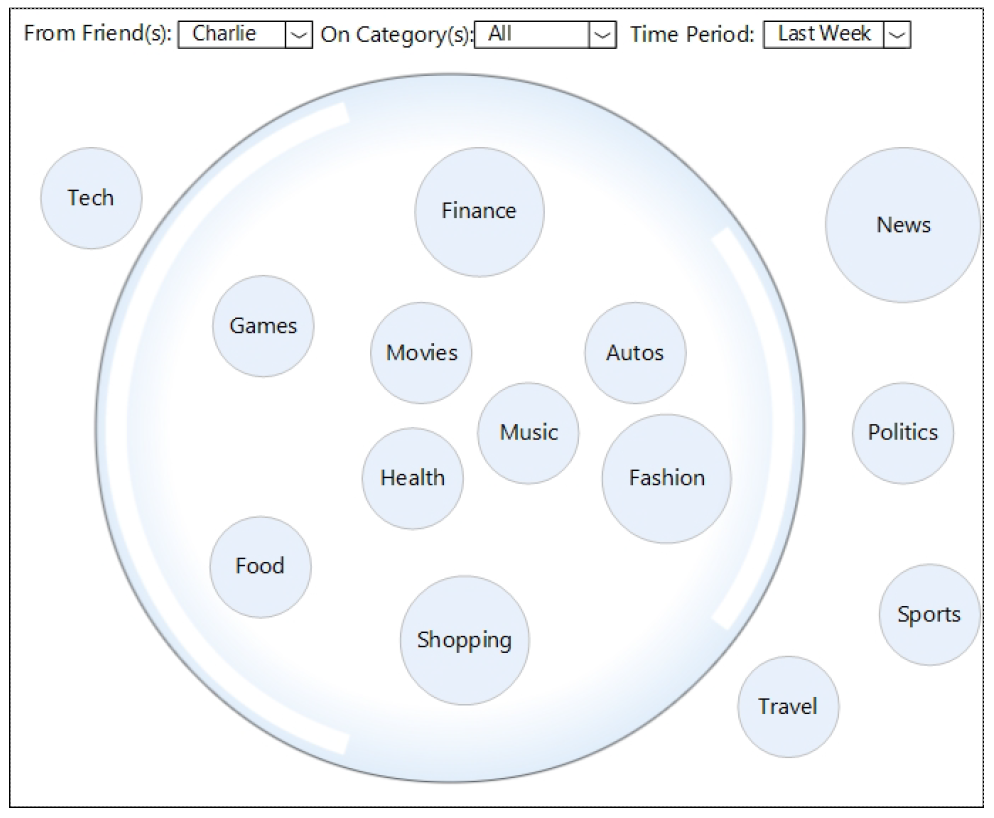
\includegraphics[keepaspectratio, width=120mm]{img/bubble_ui.png}
	% \caption{あるSNS投稿者の投稿のうち,SNSに推薦されている投稿のカテゴリと推薦されていない投稿のカテゴリの境界を可視化したシステム\protect\footnotemark[11]}
	\caption{フィルターバブルを可視化するシステム\protect\footnotemark[13]}
	\label{fig_bubble_ui}
\end{figure}
\footnotetext[13]{\cite{nagulendra_understanding_2014}より引用}

しかしこの手法では画面上に限られた数のカテゴリしか表示できない.また,このシステム自体があるアルゴリズムに基づいて投稿を選別しており,フィルターバブルを生成してしまっている.
% フィルターバブルの存在を自覚を促すことができるが,
したがって,このシステムのようにユーザインタフェースを用いて記事を推薦してしまうとフィルターバブルを生成してしまい,読者が得る情報に偏りを生んでしまうと考える.
そこで本研究では,記事の推薦にユーザインタフェースを直接は使用せず,記事や主張の文をクラスタで提示することを考える.
クラスタで提示することで,階層的に並ぶ主張の文の違いを読者の手で選別させることができる.

% フィルターバブル問題を緩和する策として,推薦アルゴリズムの公開,個人が推薦アルゴリズムを管理できるオプションの作成,UIの工夫によるバブルの可視化がある.一方で,個人が推薦アルゴリズムを微調節したところで完全に情報の泡から脱することはできないとの指摘もある.UIでバブル内外を可視化しきるのは不可能 情報が多い 手軽

% (to 提案手法)特定の地域の似た文化と価値観を持つ者同士に向けて記事を提供し,読者にコメントさせる事は,エコーチェンバー問題による情報の偏りを生むと考える.

% @see 

% \subsubsection{(トピックモデル,LSI, LDAの議論)}
% ~
% @see 

%%%%%%%%%%%%%%%%%%%%%%%%%%%%%%
% \section{(要追加調査:比較評価できる推薦手法)(出来事,主張に着目するシステムなど)}
\section{主張の文のクラスタリングを行う研究}
% ~
% @see 

\subsection{Scalable Fact-checking with Human-in-the-Loop}
\label{subsection_scalable_fact_checking}

Yangらは,ニュース読者が出来事を正確かつ迅速に把握できるように\textcolor{red}{,}
階層的クラスタリングを用いて記事に対するツイートの主張\textcolor{red}{の}グループ化\textcolor{red}{と要約を行う}手法を提案した\cite{yang_scalable_2021}.
\textcolor{red}{図\ref{fig_scalable_fact_checking_pipeline}に提案手法の概略を示す.}
この研究ではCOVID-19の話題に限定した主張の文をグループ化しているが,この手法を記事に適用した場合,多くの話題について主張のまとまりが生成されることになる.
これでは,COVID-19の飲み薬やワクチンなど異なる話題に含まれる安全性に関する共通した主張の文がグループ化されるため,読者が興味を持っている出来事の異なる主張の収集に時間を要してしまう.

\begin{figure}[H]
	\centering
	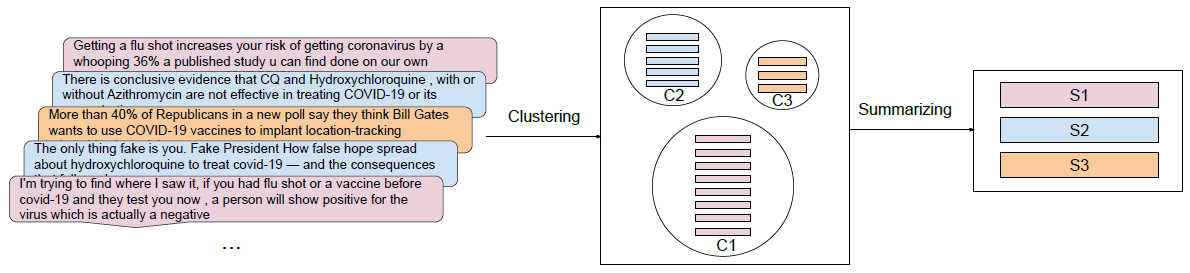
\includegraphics[keepaspectratio, width=120mm]{img/scalable_fact_checking_pipeline.png}
	\caption{
    \textcolor{red}{記事に対するツイートの主張のグループ化と要約}
    \protect\footnotemark[14]
  }
	\label{fig_scalable_fact_checking_pipeline}
\end{figure}
\footnotetext[14]{\cite{yang_scalable_2021}より引用}

\textcolor{red}{
Yangらのシステムでは,959件の記事に対する28818件のツイートを収集し,これらのツイートをクラスタ間距離0.85を閾値としてクラスタに分割していた.
このとき,全データのシルエット係数の平均が0.79となる705個のクラスタを生成しており,記事の主張を約74\%に要約できたことになる.
しかし,異なる出来事が混在した705件の主張のクラスタが提示されたときに,読者が興味を持っている出来事の異なる主張を収集することは難しい.
}

% \begin{figure}[H]
% 	\centering
% 	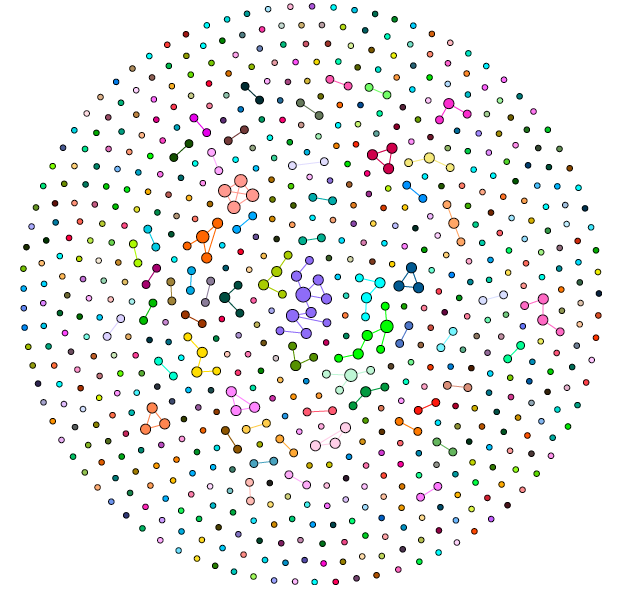
\includegraphics[keepaspectratio, width=120mm]{img/scalable_fact_checking_communities.png}
% 	\caption{
%     要約されたツイート文のコミュニティ
%     \protect\footnotemark[15]
%   }
% 	\label{fig_scalable_fact_checking_communities}
% \end{figure}
% \footnotetext[15]{\cite{yang_scalable_2021}より引用}

% TODO
% クラスタリングについて詳しく
% 図を利用
% クラスタ数が低減していないことに言及

% \subsection{Investigating COVID-19 News Across Four Nations A Topic Modeling and Sentiment Analysis Approach}
% ~
% @see 

% \subsubsection{トピックモデル,top2vec, roberta}
% ~
% @see 

%%%%%%%%%%
% \section{tf-idf -->}
% ~
% @see 
%  <!-- SCDV -->


%%%%%%%%%%%%%%%%%%%%%%%%%%%%%%%%%%%%%%%%%%%%%%%%%%%%%%%%%%%%
\chapter{提案手法}
%%%%%%%%%%%%%%%%%%%%%%%%%%%%%%%%%%%%%%%%%%%%%%%%%%%%%%%%%%%%
\label{chapter_method}

本研究では,記事の文章が出来事を述べる文と主張を述べる文に二分できると仮定する.
図\ref{fig_method_abstract}に提案手法の概要を示す.
提案手法により,より類似した出来事の異なる主張と主張に紐づく記事の推薦を行う.

\begin{figure}[H]
	\centering
	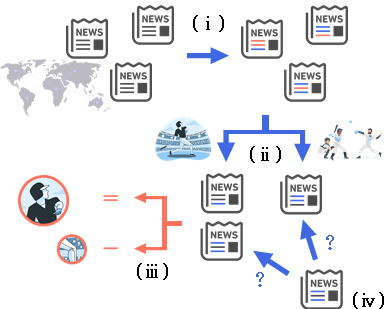
\includegraphics[keepaspectratio, width=110mm]{img/method_abstract.png}
	\caption{
    \textcolor{red}{提案手法の概要}
    \newline
    \qquad\quad(\ajroman{1})
    記事の文章を出来事の文と主張の文に分類する
    \newline
    \qquad\quad(\ajroman{2})
    出来事の文章の類似度で記事をクラスタリングする
    \newline
    \qquad\quad(\ajroman{3})
    主張の文の類似度で主張の文をクラスタリングする
    \newline
    \qquad\quad(\ajroman{4})
    読者が興味を持っている記事と最も類似した出来事を扱う記事の
    \newline
    \qquad\qquad\quad
    クラスタを同定し,そのクラスタに紐づく主張の文をクラスタご
    \newline
    \qquad\qquad\quad
    とにまとめ,記事とともに読者に提示・推薦する
  }
	\label{fig_method_abstract}
\end{figure}

第\ref{chapter_method}章は全4節で構成される.
節\ref{section_term_definition}では本研究で使用する語彙の定義を行い,
節\ref{section_method_detail}では図\ref{fig_method_abstract}に示した提案手法の詳細を説明する.
節\ref{section_select_dataset}では提案手法に必要なデータセットの選定について説明し,
節\ref{section_preprocessing_data}では選定したデータセットの前処理について説明する.

%%%%%%%%%%%%%%%%%%%%%%%%%%%%%%
\section{使用する語彙の定義}
\label{section_term_definition}
% @see 

\subsection{文と文章}
本研究では,1つの句点で区切られる文を「文」,2つ以上の文で構成される文の集合を「文章」として扱う.

\subsection{出来事と主張}
本研究では,
出来事を「記者の解釈に依存しない事象」
主張を「記者が伝えるべきだと判断した出来事の解釈」であると定義する.
すなわち,記事内の文章は出来事に対して主張を述べるような構造を持つ.
したがって,複数の出来事に対し,複数の主張が階層的に紐づいた構造を持つと考える.
% また,出来事は記者によって内容が変わりにくい出来事について先にクラスタリングを行い,

% @see 
% 話題=記事で取り上げられる出来事の対象

%%%%%%%%%%%%%%%%%%%%%%%%%%%%%%
\section{記事の出来事と主張のクラスタを用いた多様な主張を提示するニュース推薦}
\label{section_method_detail}

% \subsection{手法概要}
% ~
% @see 

% \subsection{クラスタリングの順序の検討}
% ~
% @see 

\subsection{RoBERTaを用いた出来事の文と主張の文の分類}
\label{subsection_classify_method}
出来事と主張の文の分類のため,RoBERTaを転移学習した分類器を作成した.
RoBERTaが出来事の文と主張の文の分類に適用できるよう,出来事か主張かでラベル付けされた文を含むデータセットを用いて転移学習を行った.
図\ref{fig_single_sentence_classification_of_bert}に示したように入力は文字列[CLS]と分類したい1文とし,[CLS]に対応する出力Cと正解のラベルを基に損失関数の計算を行う.
具体的には,出力Cを入力とする1層の全結合層と1ノードの出力層を接続し,その出力と\textcolor{red}{バイナリクロスエントロピー}を用いて損失を計算した.

\subsection{Sentence-BERT,コサイン距離,Ward法を用いた記事と主張の文の階層的クラスタリング}

まず,クラスタリングの前準備として「出来事と分類した文を記事ごとに結合した文章」と「主張と分類した文」のそれぞれをSentence-BERTに入力して文埋め込みを作成した.
次に,出来事の文章の埋め込みを基に記事の階層的クラスタリングを行った.
最後に,それぞれ記事のクラスタについて,主張の文の埋め込みを基に階層的クラスタリングを行った.
階層的クラスタリングを行うとき,文埋め込み間の距離の算出にはコサイン距離を使用し,この距離を基にWard法を用いてクラスタ間距離を算出した.
ここで出来事の文章の埋め込みに基づいたクラスタリングを先に行ったのは,複数の出来事に対して複数の主張が階層的に紐づいた構造を持つためである.

\subsection{k-NN分類法を用いた主張のクラスタとクラスタに紐づく記事の推薦}
まず,読者が興味を持っている記事$A$を1つ選択し,記事内の文が出来事の文であるか主張の文であるかに分類する.
この分類には小節\ref{subsection_classify_method}で作成した分類器を用いる.
次に,出来事の文を結合した文章をSentence-BERTに入力して文埋め込みを得る.
続いて,得られた埋め込みを新規のデータ,記事のクラスタの埋め込みをクラスが既知のデータとし,k-NN分類法を用いて記事$A$がどの記事のクラスタに属するかをを同定する.
最後に,同定した記事のクラスタに紐づく主張の文をクラスタごとにまとめ,記事とともに読者に提示・推薦する.

% @see 

%%%%%%%%%%%%%%%%%%%%%%%%%%%%%%
\section{データセットの選定}
\label{section_select_dataset}
% @see 

\subsection{分類器の転移学習に用いたデータセット}
追加の学習に用いるデータセットには,Wikipediaの英文をClaimを述べるかEvidenceを述べるかでラベル付けしたRinottらのIBM Debater$^{\textregistered}$ - Claims and Evidenceを利用した\cite{rinott_show_2015}.
2294個のClaimの文は「トピックを直接サポートする一般的で簡潔な文」,
4692組のEvidenceの文章は「トピックの文脈の中でClaimを直接サポートする文章」
と定義されている.
ラベル付けは5人のアノテータによって行われており,少なくとも3人が同じラベルを付与した文章を収集している.

表\ref{claim_evidence_example}にラベル付けされたClaimの文とEvidenceの文の例を示す.
Claimの文は炭素排出量のトピックについて森林伐採に焦点を当てた簡潔な説明がなされており,具体的な森林の名前を挙げずに一般の森林の話をしている.
Evidenceの文ではナイジェリアの森林面積が減少していることを具体的な数字を用いて説明しており,Claimの文を直接補っている.

\begin{table}[H]
  \caption{IBM Debater$^{\textregistered}$ - Claims and Evidenceでラベル付けされたClaimの文とEvidenceの文の例}
  \vspace{4mm}
  \centering
  \begin{tabular}{lp{12.3cm}}
    \hline
    \multicolumn{1}{c}{ラベル} & \multicolumn{1}{c}{IBM Debater$^{\textregistered}$ - Claims and Evidenceの文}
    \\
    \hline
    Claim & global carbon emissions are caused by deforestation
    % 世界の炭素排出量は森林伐採によってもたらされている
    % コンマがないのはデフォルト
    \\
    Evidence & \baselineskip=16pt
    From 1990 to 2010 Nigeria nearly halved their amount of Forest Cover, moving from 17,234 to 9041 hectares.
    % 1990年から2010年にかけて,ナイジェリアの森林面積は17,234ヘクタールから9041ヘクタールと,ほぼ半減している.
    \\[0.5mm]
    \hline
  \end{tabular}
  \label{claim_evidence_example}
\end{table}
% もう少し増やしたい

\textcolor{red}{add \textbackslash newpage}
\newpage

表の例は,本研究で定義した主張の文と出来事の文の定義と似た性質を持つ.
Claimの文は炭素排出量のトピックについて記者が伝えるべきだと判断した森林伐採の説明をしており,主張の文の定義に即している.
Evidenceの文は具体的な数字や森林のある地域名を用いて記者の解釈に依存しない事象を説明しており,出来事の文の定義に即している.
Claimの文とEvidenceの文を100件ずつ確認したところ,他の多くの例でもClaimが主張に,Evidenceが出来事に対応していた.
このことから,本研究ではClaimの文を主張の文,Evidenceの文を出来事の文として扱い,分類器の学習を行った.

% @see 

\subsection{分類とクラスタリングを行ったデータセット}
分類とクラスタリングを行うデータセットには,Ghasiyaらが収集したCOVID-19 News Articlesを選定した\textcolor{red}{\cite{ghasiya_investigating_2021}}.
表\ref{covid_19_news_articles_composition}示すように,COVID-19 News Articlesはイギリス,インド,日本,韓国の主要な新聞8紙の英語版ウェブサイトから約10万件の記事を収集している.
これらの記事は,スクレイピングライブラリBeautiful Soupを用いて収集された記事のうち文字列COVID-19またはCoronavirusを含む記事である.
このうちイギリスの記事には句点が含まれておらず,文章を文に分割できなかったため使用しなかった.

\begin{table}[H]
  \caption{COVID-19 News Articlesの構成}
  \centering
  \vspace{4mm}
  \begin{tabular}{ccc}
    \hline
    Countries & Newspapers & No. of Articles \\
    \hline
    UK & The Daily Mail & 23,821 \\
    India & Hindustan Times, The Indian Express & 47,342 \\
    Japan & The Japan Times, Asahi Shimbun, Mainichi Shimbun & 21,039 \\
    South Korea & Korea Herald, Korea Times & 10,076 \\
    \hline
    \end{tabular}
  \label{covid_19_news_articles_composition}
\end{table}

\newpage

COVID-19 News Articlesは3ヶ国の英記事が含まれるため,政治や文化の違いに由来する多くの異なる主張が分析できると考えた.
加えてCOVID-19に関連する出来事は記者によって多くの異なる主張が記されているため,分析に適していると考えた.
また,このデータセットは2020年1月1日から2020年12月1日の11カ月間という短い期間で収集されているため,より類似した出来事に関する記事が得られると期待できる.
Yangらの研究と同様に話題がCOVID-19に限定されてしまっているが,限定された話題でも同じ出来事の異なる主張がクラスタリングされる様子は観測できると考えた.
% @see weekly-report_20210930.md

%%%%%%%%%%%%%%%%%%%%%%%%%%%%%%
\section{データの前処理}
\label{section_preprocessing_data}
% @see 

\subsection{自然言語処理のためのテキストの前処理}
IBM Debater$^{\textregistered}$ - Claims and EvidenceとCOVID-19 News Articlesの文章に対し,小節\ref{subsection_texts_preprocessing}で述べたような単語の表記揺れを少なくするいくつかの前処理を行った.
具体的な処理は小節\ref{subsection_data_preprocessing_implement}で説明する.

% @see 
% \subsection{テキストの前処理}
% 単語埋め込みのように,自然言語処理ではテキストをコンピュータが解釈しやすい数値に変換して処理することが多い.
% このとき,コンピュータはテキストを文字の羅列としか見ていないため,Appleとappleを別の単語と見なし,違う数値に変換してしまう.
% このような単語の表記揺れは,文章中の単語の出現頻度の情報を不正確なものにする.
% 表記揺れによって増加した出現頻度の少ない単語が学習のノイズとなってしまうこともある.
% 従って,テキストに何らかの処理をする前に,大文字を小文字に変換するなどの表記揺れを解消する処理を行う必要がある.
% URLやメールアドレスといったユニークな文字の羅列は,出現頻度が極めて少ないノイズとなり得るため,事前に除去しておくと良い.

\textcolor{red}{add \textbackslash newpage}
\newpage

\subsection{省略のピリオドなどを考慮した文章の分割}
記事の文を分類するにあたり,文章を文ごとに分割する必要がある.
しかし,表\ref{period_usecase}のように英語の句点に用いられるピリオドは句点以外にも様々な用法があり,人間が決めたアルゴリズムによる文章の分割が難しい\cite{kreuzthaler_detection_2015}.
% F1スコア
% 1117
% @see weekly-report-20211110-1215
\begin{table}[H]
  \caption{英語のピリオドの用例}
  \centering
  \vspace{4mm}
  % \begin{tabular}{cp{12.3cm}}
  \begin{tabular}{cl}
    \hline
    種類 & \multicolumn{1}{c}{例} \\
    \hline
    文頭の省略語 & Prof. Kimura studies. \\
    文中の省略語 & Alphabets e.g. A, B, C. \\
    文末の省略語 & The tail of a bull, cow, ox etc. \\
    日付 & 25.01.2022. \\
    ファイル名 & readme.txt \\
    URL & \text{http://www.wikipedia.org} \\
    IPアドレス & 127.0.0.1. \\
    メールアドレス & abc@shibaura-it.ac.jp \\
    分類コード & A01.9 \\
    \hline
    \end{tabular}
  \label{period_usecase}
\end{table}
% これ全部が解決できたことを確認していない

そこで,テキスト解析のための機械学習ライブラリStanzaを用いて句点としてのピリオドの位置を同定した\cite{qi_stanza_2020}.
他のテキスト解析のツールとしてUDPipeやspaCyも広く用いられているが,2018 UD Shared Taskの英語の句点の同定におけるスコアはStanzaが最も優れている.

%%%%%%%%%%%%%%%%%%%%%%%%%%%%%%%%%%%%%%%%%%%%%%%%%%%%%%%%%%%%
\chapter{実装}
%%%%%%%%%%%%%%%%%%%%%%%%%%%%%%%%%%%%%%%%%%%%%%%%%%%%%%%%%%%%
\label{chapter_implement}
実験では,主張の文の階層的クラスタリングまでを行うシステムを実装し,より類似した出来事の異なる主張の文を提示できているかを評価した.
第\ref{chapter_implement}章では,実験に用いたシステムの実装について説明する.
節\ref{section_system_plan}ではシステムの入出力やデータフローなどの設計指針を説明し,
節\ref{section_environment}では使用したコンピュータの構成やツールについて説明し,
節\ref{section_system_implement}では具体的なシステムの実装方法について説明する.


%%%%%%%%%%%%%%%%%%%%%%%%%%%%%%
\section{システムの設計指針}
\label{section_system_plan}
提案手法を実装するシステムは,入力を「読者が興味を持っている1件の記事」とし,出力を「入力した記事と最も類似した出来事を扱う記事のクラスタに紐づく複数の主張の文」と「出力する主張の文の抽出元である記事」とした.
また,分類器の学習のためにIBM Debater$^{\textregistered}$ - Claims and Evidenceを,クラスタの作成のためにCOVID-19 News Articlesを使用した.

COVID-19 News Articlesから生成した記事のクラスタ群と主張の文のクラスタ群は,クラスタごとにテキストファイルに保存した.
COVID-19 News Articlesの各記事には,主張の文から記事を特定するための固有のIDと記事の出来事の文章から生成した文埋め込みの情報を付与した.
また,各文には文に固有のIDと抽出元の記事のID,出来事か主張かのラベル,文埋め込みの情報を付与した.
% 実験では分類とクラスタリングの実装を行い,これらの評価を行った.

% @see 

%%%%%%%%%%%%%%%%%%%%%%%%%%%%%%
% \section{システム構成(モジュールの説明)}
% 後回し,もしくは除去
% @see 

%%%%%%%%%%%%%%%%%%%%%%%%%%%%%%
\section{実行環境}
\label{section_environment}
本システムの実行には,表\ref{pc_spec}に示す構成のコンピュータと表\ref{module_version}に示す
ツール
% プログラミング言語やライブラリ
を用いた.

\begin{table}[H]
  \caption{実行したコンピュータの構成}
  \centering
  \vspace{4mm}
  % \begin{tabular}{cp{12.3cm}}
  \begin{tabular}{cl}
    \hline
    項目 & \multicolumn{1}{c}{詳細} \\
    \hline
    OS & Ubuntu (Version 18.04) \\
    CPU & Intel$^{\textregistered}$ Core$^{TM}$ i5-7640X (4.00GHz, 4コア) \\
    GPU & GeForce RTX 3070 (1500MHz, 8GB,
    % https://gamingpcs.jp/hikaku/hikaku_gpu/geforce-rtx3070/
    % CUDAコア数5888,
    CUDA Version 11.5) \\
    メモリ & 2667 MT/s 16GB $\times$ 2枚 \\
    ストレージ & HDD 1815 Mbit/s \\
    % https://toshiba.semicon-storage.com/jp/storage/product/internal-specialty/pc/articles/dt01aca-series.html
    マザーボード & X299チップセット \\
    % https://www.asrock.com/mb/intel/X299%20Extreme4/index.jp.asp
    \hline
    \end{tabular}
  \label{pc_spec}
\end{table}

% https://qiita.com/DaisukeMiyamoto/items/98ef077ddf44b5727c29

\begin{table}[H]
  % \caption{使用したプログラミング言語とライブラリとそのバージョン}
  \caption{使用したツール}
  \centering
  \vspace{4mm}
  % \begin{tabular}{cp{12.3cm}}
  \begin{tabular}{lll}
    \hline
    \multicolumn{1}{c}{項目} & \multicolumn{1}{c}{バージョン} & \multicolumn{1}{c}{用途} \\
    \hline
    GNU Awk & 4.1.4 & テキストの前処理 \\
    Python & 3.6.9 & GNU gawk以外のプログラムの実行 \\
    Stanza & 1.3.0 & 文章の文への分割 \\
    pandas & 1.1.5 & 分類器に合わせたデータの入力形式の変更 \\
    Simple Transformers & 0.63.3 & RoBERTAを用いた分類器の作成 \\
    PyTorch & 1.8.2 $+$ cu111 & Simple Transformerの内部処理 \\
    SentenceTransformers & 2.1.0 & Sentence-BERTを用いた文埋め込みの作成 \\
    scikit-learn & 0.24.2 & 混同行列を用いた評価指標の算出 \\
    LibreOffice Calc & 7.2.5.2 & 混同行列を用いた評価指標の算出 \\
    SciPy & 1.5.4 & 階層的クラスタリングの実行と結果の可視化 \\
    \hline
    \end{tabular}
  \label{module_version}
\end{table}

% @see experiment/logs/tools_*.log

%%%%%%%%%%%%%%%%%%%%%%%%%%%%%%
\section{システムの実装}
\label{section_system_implement}

\subsection{GNU Awkを用いたテキストの前処理の実装}
\label{subsection_data_preprocessing_implement}
GNU Awkは,あるパターンに従う文字列を検索し,他の文字列に置換するなどの処理を行えるプログラミング言語である.
文字列のパターンは,正規表現と呼ばれる表現形式で別の文字列を用いて表すことができる.

2つのデータセットIBM Debater$^{\textregistered}$ - Claims and EvidenceとCOVID-19 News Articlesについて,小節\ref{subsection_texts_preprocessing}で述べた単語の表記揺れやノイズを少なくするため,GNU Awkと正規表現を用いて以下の処理を順に行った.

\begin{multicols}{2}
  \begin{enumerate}
  \item 大文字の小文字化
  \item 改行文字の除去
  \item タブ文字の除去
  \item 改行文字の除去
  \item 特殊な空白文字(no break space,thin space)の除去
  \item 絵文字の除去
  \columnbreak
  \item URLの除去
  \item メールアドレスの除去
  \item 英数字,空白文字,句読点以外の文字の除去
  \item ピリオド,疑問符,感嘆符の前の空白文字の除去
  \item 2つ以上の空白文字を1つの空白文字に置換
  \item 行頭の1つ以上の空白文字,ピリオド,疑問符,感嘆符の除去
  \end{enumerate}
\end{multicols}

また,この2つのデータセットで文の形式を合わせるため,IBM Debater$^{\textregistered}$ - Claims and Evidenceの文の末尾にピリオドを追加した.
加えて,IBM Debater$^{\textregistered}$ - Claims and Evidenceの文のみに含まれていた特殊な文字列[REF]を除去した.

% awk の基本的な機能は,あるパターンを含む行 (あるいはその他のテキスト単位) をファイルから探し出すことです.行がパターンの 1 つにマッチすると,awk はその行に対して指定された処理を行います.awk は入力ファイルの最後に達するまで,この方法で入力行を処理し続けます.
% @see https://www.gnu.org/software/gawk/manual/gawk.html

\subsection{Stanzaを用いた文章を文単位に分割する実装}
PythonライブラリであるStanzaを使用し,IBM Debater$^{\textregistered}$ - Claims and Evidenceの出来事の文章とCOVID-19 News Articlesの文章の句点としてのピリオドの位置を同定した.その後,同定したピリオドの後ろに改行文字を挿入した.
分割した出来事の文や主張の文には重複する文の組が多く見受けられたため,重複する文は1文を残して
% Pythonで
除去した.
% uniqueの{}

\textcolor{red}{
  Stanzaの英語版モデルには,ウェブログ,ニュース文,メール文,レビュー文,Yahoo! answersの16621文とそのテキスト解析結果を含むデータセットUD English EWTを学習したモデルを使用した. 
}

% @see https://stanfordnlp.github.io/stanza/available_models.html
% @see https://universaldependencies.org/treebanks/en_ewt/index.html
% @see https://paperswithcode.com/paper/stanza-a-python-natural-language-processing/review/
% ライセンスは[Attribution-ShareAlike 4.0 International (CC BY-SA 4.0) ](https://creativecommons.org/licenses/by-sa/4.0/) 

% (Stanza, spacyの議論)
% @see 

%%%%%%%%%%%%%%%%%%%%%%%%%%%%%%
\subsection{RoBERTaを用いた出来事の文と主張の文の分類器の実装}
\textcolor{red}{
RoBERTaの事前学習モデルにはLiuらのRoBERTa baseを利用した\cite{liu_roberta_2019}.
RoBERTa baseは1層に16個のScaled Dot-Product Attentionを含むTransformerエンコーダを768個持つ層を12層用いている.
% 125Mパラメータ
また,ニュース記事を含む約160GBの英文をバッチサイズ8,000で50万回学習している.
}
% 英語
% 大文字と小文字を区別するらしい...
% The model was trained on 1024 V100 GPUs for 500K steps with a batch size of 8K and a sequence length of 512. The optimizer used is Adam with a learning rate of 6e-4, β1=0.9\beta_{1} = 0.9β1​=0.9, β2=0.98\beta_{2} = 0.98β2​=0.98 and ϵ=1e−6\epsilon = 1e-6ϵ=1e−6, a weight decay of 0.01, learning rate warmup for 24,000 steps and linear decay of the learning rate after.
% @see https://huggingface.co/roberta-base
% 12-層,768-隠れ次元,16-ヘッド,125M パラメータ
% @see https://tensorflow.classcat.com/2021/05/16/huggingface-transformers-4-6-pretrained-models/
% @see https://github.com/pytorch/fairseq/tree/main/examples/roberta

% 2層とRoBERTaを学習した
% class RobertaClassificationHead(nn.Module):
%     """Head for sentence-level classification tasks."""
%     def __init__(self, config):
%         super().__init__()
%         self.dense = nn.Linear(config.hidden_size, config.hidden_size)
%         self.dropout = nn.Dropout(config.hidden_dropout_prob)
%         self.out_proj = nn.Linear(config.hidden_size, config.num_labels)

RoBERTa baseの転移学習と分類の実行には,PythonライブラリであるSimple Transformersを使用した.
Simple Transformersの内部では同じくPythonのライブラリであるPyTorchが用いられている.

転移学習ではIBM \textcolor{red}{Debater} - Claims and Evidenceの出来事の文と主張の文のそれぞれについて8割を訓練データ,2割をテストデータに分割し,バイナリクロスエントロピーの計算を行った.
このとき,データの順序に由来する不必要な学習を回避するため,文とラベルは疑似乱数を用いた無作為な順序で学習した\cite{aurellen20}.
% random.shuffle
% @see p.127 412
また,出来事の文は4209文,主張の文は2169文と数が不均衡であるため,出来事の文の学習の重みに$\frac{2169}{4209}$を乗算し,
% 出来事の文を学習しにくくした.
ラベルごとに均等に学習ができるようにした.
学習のバッチサイズは40文とし,その他の学習のパラメータはSimple Transformersのデフォルトの値を使用した.

% 回数を変えて学習したとき,バイナリクロスエントロピーの値は2エポックで約0.207,3エポックで約0.237,4エポックで約0.297,12エポックで約0.590と単調増加していた.
% つまり,

学習した分類器にCOVID-19 News Articlesの文を入力し,分類したラベル,記事のID,文のIDとともにテキストファイルに保存した.
分類結果はPythonライブラリであるscikit-learn,Simple Transformersと表計算ソフトであるLibreOffice Calcを用いて混同行列として集計し,これを基に適合率,再現率,マシューズ相関係数を計算した.

%%%%%%%%%%%%%%%%%%%%%%%%%%%%%%
\subsection{Sentence-BERTを用いた文埋め込みを生成する実装}
出来事の文は記事に記載された順序で記事ごとに結合し,Sentence-BERTに入力した.
% 文脈情報の保存
% 本当はリストに格納して1回渡すだけ
文の間には空白文字を挿入して結合した.
% 実際の文章と同様に
出来事の文章を基に生成した文埋め込みは記事のIDと紐づけてテキストファイルに保存した.
主張の文は1文ずつSentence-BERTに入力し,文のIDと紐づけてテキストファイルに保存した.
% 本当はリストに格納して1回渡すだけ


\textcolor{red}{
Sentence-BERTのモデルにはRaimersらのparaphrase-MiniLM-L6-v2を使用した\cite{reimers_sentence-bert_2019}.
paraphrase-MiniLM-L6-v2は1層に12個のScaled Dot-Product Attentionを含むTransformerエンコーダを384個持つ層を6層用いている.
% 125Mパラメータ
MNLIとSNLI(The Stanford Natural Language Inference)の約100万文のうち約10万文の英文をバッチサイズ16で1回学習している.
MNLIは話し言葉と書き言葉の様々な英文をカバーしている.
}
% {
%   "_name_or_path": "old_models/paraphrase-MiniLM-L6-v2/0_Transformer",
%   "architectures": [
%     "BertModel"
%   ],
%   "attention_probs_dropout_prob": 0.1,
%   "gradient_checkpointing": false,
%   "hidden_act": "gelu",
%   "hidden_dropout_prob": 0.1,
%   "hidden_size": 384,
%   "initializer_range": 0.02,
%   "intermediate_size": 1536,
%   "layer_norm_eps": 1e-12,
%   "max_position_embeddings": 512,
%   "model_type": "bert",
%   "num_attention_heads": 12,
%   "num_hidden_layers": 6,
%   "pad_token_id": 0,
%   "position_embedding_type": "absolute",
%   "transformers_version": "4.7.0",
%   "type_vocab_size": 2,
%   "use_cache": true,
%   "vocab_size": 30522
% }

% MRPC.並列するニュースソースからMicrosoft Research Paraphrase Cor-pus (Dolan et al., 2004)を抽出.

% SNLI (Bowman et al., 2015) と Multi-Genre NLI (Williams et al., 2018) のデータセットの組み合わせでSBERTを学習させる.SNLIは,contradiction,eintailment,neu-tralのラベルでアノテーションされた57万文のペアのcol-lectionである.MultiNLIは43万文のペアを含み,話し言葉と書き言葉の様々なジャンルをカバーしています.SBERTを3ウェイソフトマックス分類器の目的関数で1エポック分微調整した.バッチサイズ16,学習率2e-5のアダムオプティマイザを用い,学習データの10%に渡って線形学習率のウォームアップを行った.デフォールトプーリング戦略はMEANである.

% シャッフル
% @see https://www.google.com/url?sa=t&rct=j&q=&esrc=s&source=web&cd=&cad=rja&uact=8&ved=2ahUKEwjs26WKr8r1AhWQzpQKHXpCBDcQFnoECAoQAQ&url=https%3A%2F%2Fhuggingface.co%2Fsentence-transformers%2Fparaphrase-MiniLM-L6-v2&usg=AOvVaw0vPzyNJ5AtBMiIa-USrve7
% @see https://www.sbert.net/docs/pretrained_models.html
% @see https://huggingface.co/sentence-transformers/paraphrase-MiniLM-L6-v2/blob/main/config.json
% @see 

\textcolor{red}{add \textbackslash newpage}
\newpage

%%%%%%%%%%%%%%%%%%%%%%%%%%%%%%

\subsection{コサイン距離とWard法を用いた記事の階層的クラスタリングの実装}
記事のIDに紐づけられた出来事の文章の文埋め込みを基に,PythonライブラリであるSciPyを用いて埋め込みの距離行列を作成した.
この距離行列は,i番目の埋め込みとj番目の埋め込みとの距離をi行j列に格納した行列である.
距離行列を作成することで,これらの距離を複数回参照するときにコンピュータの計算資源を節約することができる.

次に,SciPyと距離行列を用いてWard法によるクラスタ間距離を計算し,階層的クラスタリングを行った.
$n$回のクラスタの結合を行う階層的クラスタリングの結果は,$n$行4列の行列として保存される.
1列目と2列目には結合される2つのクラスタのID,3列目には2つのクラスタ間距離,4列目には新しく生成されるクラスタのIDが保存される.

最後に,SciPyと保存された階層的クラスタリングの結果を使用してデンドログラムを作図し,データの分析を行った.

% @see 

%%%%%%%%%%%%%%%%%%%%%%%%%%%%%%
\subsection{コサイン距離とWard法を用いた主張の文の階層的クラスタリングの実装}
まず,記事の階層的クラスタリングで生成した各クラスタに対し,クラスタ内の各文のIDに紐づけられた分類結果の情報を参照し,主張の文のみを抽出した.
その後,文のIDに紐づけられた文埋め込みを参照し,各クラスタについて埋め込みの距離行列の作成,階層的クラスタリングの実行,デンドログラムの作図を行った.
% @see 


%%%%%%%%%%%%%%%%%%%%%%%%%%%%%% 
% \section{仮説}
% @see 
%  評価実験を設計するにあたり以下3件の仮説を立てる.
% \begin{itemize}
%   \item 仮説1) .
%   \item 仮説2) 
%   \item 仮説3) 
% \end{itemize}
% この3件の仮設は,それぞれ以下の考察に基づき設定されている.
% 仮説1は...


%%%%%%%%%%%%%%%%%%%%%%%%%%%%%%%%%%%%%%%%%%%%%%%%%%%%%%%%%%%%
\chapter{実験}
%%%%%%%%%%%%%%%%%%%%%%%%%%%%%%%%%%%%%%%%%%%%%%%%%%%%%%%%%%%%
\label{chapter_experiment}

第\ref{chapter_experiment}章では,第\ref{chapter_implement}章で述べた分類器とクラスタリングの実験について説明する.
節\ref{section_ibm_classification_experiment}ではIBM Debater$^{\textregistered}$ - Claims and Evidenceのテストデータを用いた分類器の実験について説明し,
節\ref{section_covid_classification_experiment}ではCOVID-19 News Articlesを用いた分類器の実験について説明する.
その後,節\ref{section_article_clustering_experiment}で記事の階層的クラスタリングの実験について説明し,
節\ref{section_sentence_clustering_experiment}で主張の文の階層的クラスタリングの実験について説明する.

%%%%%%%%%%%%%%%%%%%%%%%%%%%%%%
\section{IBM Debater$^{\textregistered}$ - Claims and Evidenceのテストデータを用いた分類器の実験}
\label{section_ibm_classification_experiment}
% @see 

\subsection{実験方法}
分類器の最適なエポック数を決定するため,IBM Debater$^{\textregistered}$ - Claims and Evidenceの2割のテストデータを使用し,学習ごとのバイナリクロスエントロピーと分類結果の適合率,再現率,マシューズ相関係数を確認した.
適合率,再現率,マシューズ相関係数の計算では,出来事の文と比べてデータ数が少ない主張の文のラベルを陽性クラスとした.
% @see 

\subsection{実験結果}
表\ref{ibm_classification_evaluation}にエポック数ごとの分類器の評価を示す.
どのエポック数でも適合率,再現率,マシューズ相関係数の値が0.81と大きく,モデルが分類器として機能していることがわかる.
バイナリクロスエントロピー,適合率,マシューズ相関係数は1エポックで,再現率は3エポックで最も優れた値となった.
バイナリクロスエントロピーが単調増加しているため,学習するほどモデルが訓練データに対して過学習してしまう可能性がある.

\begin{table}[H]
  \caption{
    エポック数ごとの分類器の評価(小数第3位を四捨五入)
    }
  \centering
  \vspace{4mm}
  % {\tabcolsep=0.15cm
    \begin{tabular}{ccccccc}
    \hline
    評価指標 & $1$ epoch & $2$ epochs & $3$ epochs & $4$ epochs & $12$ epochs & $100$ epochs
    \\
    \hline
    BCE & $\mathbf{0.17}$ & $0.21$ & $0.24$ & $0.30$ & $0.59$ & $0.87$
    \\
    適合率 & $\mathbf{0.90}$ & $0.86$ & $0.86$ & $0.86$ & $0.85$ & $0.85$
    \\
    再現率 & $0.89$ & $0.90$ & $\mathbf{0.92}$ & $0.89$ & $0.89$ & $0.91$
    \\
    MCC & $\mathbf{0.84}$ & $0.82$ & $0.83$ & $0.82$ & $0.81$ & $0.82$
    \\
    \hline
    \end{tabular}
  % }
  \label{ibm_classification_evaluation}
\end{table}
% 1{'mcc': 0.8387780193426857, 'tp': 376, 'tn': 808, 'fp': 43, 'fn': 48, 'auroc': 0.977416967829191, 'auprc': 0.9476252884837162, 'eval_loss': 0.1677857233898976, 'acc': 0.9286274509803921}
% 2{'mcc': 0.8173129764924434, 'tp': 382, 'tn': 788, 'fp': 63, 'fn': 42, 'auroc': 0.9713835554175998, 'auprc': 0.9251588809193649, 'eval_loss': 0.2068871846249749, 'acc': 0.9176470588235294}
% 3{'mcc': 0.8306606574490791, 'tp': 389, 'tn': 788, 'fp': 63, 'fn': 35, 'auroc': 0.9674314901447797, 'auprc': 0.8984210954225702, 'eval_loss': 0.2356283680874185, 'acc': 0.9231372549019607}
% 4{'mcc': 0.8164008811069239, 'tp': 379, 'tn': 791, 'fp': 60, 'fn': 45, 'auroc': 0.9706338824468438, 'auprc': 0.9305744848173877, 'eval_loss': 0.2970533335633263, 'acc': 0.9176470588235294}
% 12{'mcc': 0.8061959453861247, 'tp': 377, 'tn': 787, 'fp': 64, 'fn': 47, 'auroc': 0.961162505820012, 'auprc': 0.8900233134115612, 'eval_loss': 0.5898509680812367, 'acc': 0.9129411764705883}
% 100{'mcc': 0.8155391227971583, 'tp': 386, 'tn': 782, 'fp': 69, 'fn': 38, 'auroc': 0.960870119504246, 'auprc': 0.9106979966867893, 'eval_loss': 0.8653483360831373, 'acc': 0.9160784313725491}
% 陽性=tp+fn=424で少数クラス(主張の文)となっている
% 主張の文2169*0.2=433.8!=424となるのが謎

\subsection{実験の考察}
バイナリクロスエントロピーが単調増加しているため,多くのエポック数で学習した分類器はCOVID-19 News Articlesでの分類精度が悪くなると考えられる.
したがって,14エポックと100エポックで学習したモデルは除外して考える.

一方でエポック数が少なすぎるとモデルの学習不足で過少適合となる可能性があり,同じくCOVID-19 News Articlesでの分類精度が悪くなると考えられる.
したがって,2エポックや4エポックのモデルが最も精度よくCOVID-19 News Articlesの分類を行う可能性は捨てきれない.

1エポックから4エポックにかけて適合率,再現率,マシューズ相関係数の差は最大で0.04と小さいため,この4つの学習済みモデルでCOVID-19 News Articlesの分類精度を検証することにした.

%%%%%%%%%%%%%%%%%%%%%%%%%%%%%%
\section{COVID-19 News Articlesを用いた分類器の実験}
\label{section_covid_classification_experiment}
~
% @see 

\subsection{実験方法}
IBM Debater$^{\textregistered}$ - Claims and Evidenceを1,2,3,4エポック学習した4つの分類器について,COVID-19 News Articlesの分類結果から適合率,再現率,マシューズ相関係数を算出した.
COVID-19 News Articlesの正解ラベルには,3ヶ国の記事から3件ずつ記事を抽出した計163個の文を手動でラベル付けしたものを用いた.
ラベル付けを行うにあたり,IBM Debater$^{\textregistered}$ - Claims and Evidenceの出来事の文と主張の文をそれぞれ100文ずつ分析し,ラベル付けの基準を作成した.
適合率などの計算では,分類結果においても正解ラベルにおいても主張の文が出来事の文より少なかったため,主張の文のラベルを陽性クラスとした.

% @see 

\textcolor{red}{add \textbackslash newpage}
\newpage

\subsection{実験結果}
表\ref{covid_classification_criterion}にIBM Debater$^{\textregistered}$ - Claims and Evidenceの分析を基に作成したラベル付けの基準を示す.
この基準に従い,COVID-19 News Articlesの163文のラベル付けを行った.
% 基準がダブる場合は?

\begin{table}[H]
  \centering
  \caption{
    COVID-19 News Articlesのラベル付けの基準
    % \newline
    % \qquad~
    (E : 出来事の文,
    % \newline
    C : 主張の文)
    }
    \centering
  \vspace{4mm}
  % {\tabcolsep=0.15cm
    \begin{tabular}{cp{4cm}p{8cm}}
    \hline
    ラベル & \multicolumn{1}{c}{基準} & \multicolumn{1}{c}{IBM Debater$^{\textregistered}$ - Claims and Evidenceの例文}
    \\
    \hline
    E
    & \baselineskip=16pt
    記者の解釈に依存しない事実を述べている
    & \baselineskip=16pt
    \textbf{michael martin was the first eu foreign minister to enter gaza in over a year}
    \\[2mm]
    & \baselineskip=16pt
    指示語を含み,別の文を補助している
    & \baselineskip=16pt
    in \textbf{his} book maybe one bill mckibben argues in favor of a one child policy based on \textbf{this} research
    \\[2mm]
    & \baselineskip=16pt
    具体的な事物の数値を含む
    & \baselineskip=16pt
    in \textbf{2020} total gross foreign aid to all developing countries was \textbf{76 billion}.
    \\[2mm]
    C
    & \baselineskip=16pt
    事実に対する解釈を述べている
    & \baselineskip=16pt
    this is the most \textbf{technologically advanced} and \textbf{safest} \textbf{pipeline} ever proposed.
    \\[2mm]
    & \baselineskip=16pt
    主語や述語の一般性が高い
    & \baselineskip=16pt
    \textbf{gamblers persist in gambling} even after repeated losses.
    \\[2mm]
    % & \baselineskip=16pt
    % 主語が筆者である
    % & \baselineskip=16pt
    % \\[0.5mm]
    \hline
    \end{tabular}
  % }
  \label{covid_classification_criterion}
\end{table}

% @see weekly report 20211229
% - C
% - 主語がデカい
%     - 筆者の考え
%     - 固有名詞,特定の1つでない
% - 論文の文頭にきそう
% - 長い文もある
% - 言い切り
% - 「また,」
% - ~だったら~
% - ~でしょう
% - ~は当然だ
% - 事実を語るだけでなく,事実に対する説明を行っている
% - E
% - 指示語
% - その結果
%     - Cによる影響
% - 数字
% - 事実
% -   判明した
% - 補助的でベクトルの異なる情報が多い
% - ~を求めている
% - を遺憾に思う
% - 主張がある事実を客観視する文
%     - メインの主張ではないのかも
%     - 主張の文節の後に事実の文節
% - 別の人も似たようなことを言っている という文
%     - メインの主張と似た事を挿すため,代表の主張にする必要はない
%     - 出来事のクラスタリングに混ぜるのも悪すぎはしない?
%     - 誰かが何かを話しているという「事実」
% - 決意表明157
% - 100文に2文ほど1行2文が存在
%     - DeepLによるエラー

\textcolor{red}{add \textbackslash newpage}
\newpage

表\ref{covid_classification_evaluation}にCOVID-19 News Articlesの163文の分類の評価結果を示す.
適合率,再現率,マシューズ相関係数の全てにおいて3エポックの分類器が最も優れていた.
3エポックの分類器は再現率が低いが,適合率とマシューズ相関係数が高く,分類器として機能していることがわかる.
3エポックの分類器が主張の文を出来事の文と誤分類することは1度もなく,適合率は1となっている.
以降の説明では,全てこの3エポックの分類器を用いた実験の結果を記す.

\begin{table}[H]
  \caption{
    COVID-19 News Articlesの163文の分類の評価(小数第3位を四捨五入)
  }
  \centering
  \vspace{4mm}
  % {\tabcolsep=0.15cm
    \begin{tabular}{ccccc}
    \hline
    評価指標 & $1$ epoch & $2$ epochs & $3$ epochs & $4$ epochs
    \\
    \hline
    TP & $3$ & $4$ & $6$ & $5$
    \\
    TN & $146$ & $148$ & $148$ & $147$
    \\
    FP & $2$ & $0$ & $0$ & $1$
    \\
    FN & $12$ & $11$ & $9$ & $10$
    \\
    適合率 & $0.60$ & $\mathbf{1.00}$ & $\mathbf{1.00}$ & $0.83$
    \\
    再現率 & $0.20$ & $0.27$ & $\mathbf{0.40}$ & $0.33$
    \\
    MCC & $0.31$ & $0.50$ & $\mathbf{0.61}$ & $0.50$
    \\
    \hline
    \end{tabular}
  % }
  \label{covid_classification_evaluation}
\end{table}

\textcolor{red}{add \textbackslash newpage}
\newpage

表\ref{covid_classification_example}に分類結果の例を示す.
5つ目の文は,一般の家族や教育者にいえる筆者の解釈が述べられているが,出来事に誤分類されていた.
6つ目の文は,一般のオンライン授業にいえる事実(them)に対する筆者(i)の解釈が述べられているが,出来事に誤分類されていた.


\begin{table}[H]
  \caption{分類器の主張の文 ($C$)と出来事の文($E$)の分類例}
  \vspace{4mm}
  \centering
  {\tabcolsep=0.1cm
  \begin{tabular}{ccp{10.5cm}}
      \hline
      正解ラベル & 分類結果 & \multicolumn{1}{c}{COVID-19 News Articlesの文}
      \\
      \hline
      $C$ & $C$ & \baselineskip=16pt
      the goal was to bolster international competitiveness.
      % 国際的な競争力を強化するためです.
      \\[2mm]
      % JP69
      $C$ & $C$ & \baselineskip=16pt
      proponents see the pandemic as a chance to break with the modern calendar.
      % パンデミックは現代のカレンダーと決別するチャンスだと考えています
      % JP42
      \\[2mm]
      $E$ & $E$ & \baselineskip=16pt
      the government is reportedly aiming to announce guidance early next month.
      \\[2mm]
      % JP81
      % 政府は来月初めにガイダンスを発表することを目指していると言われています
      $E$ & $E$ & \baselineskip=16pt
      over 20000 people have signed an online petition calling for a shift to september school starts.
      % 9月入学への移行を求めるオンライン署名に2000人以上が参加しました.
      % JP54
      \\[2mm]
      $E$ & $C$ & \baselineskip=16pt
      for now there is little that families and educators can do but wait to see what the abe administration has in mind.
      % 今のところ,家族や教育者ができることは,ABE政権が何を考えているかを待つことだけです
      % JP80
      \\[2mm]
      $E$ & $C$ & \baselineskip=16pt
      i dont think online classes can completely replace them
      % オンライン授業が完全に代替できるとは思えません.
      % JP60
      \\[1mm]
      \hline
    \end{tabular}
    \label{covid_classification_example}
    }
\end{table}


\subsection{実験の考察}
分類の適合率が極めて大きいため,2019年の最先端のモデルであるRoBERTaが適切に転移学習できたと考える.
一方で再現率は学習時よりも0.52と大幅に下がっており,分類器が訓練データに過学習している可能性がある.

再現率の改善のため,学習と分類に用いたデータセットの違いをより詳細に分析し,手法を見直す必要がある.
学習に用いたデータセットでは指示語が含まれる文を出来事の文とすることが多かったのに対し,表\ref{covid_classification_example}で出来事と誤分類した主張の文には指示語に用いられる``there''が含まれていた.
しかし,誤分類した文では``there is''という構文で用いられ,指示語として``there''を用いていない.
したがって,このような構文を加味した分類を行うことにより再現率の向上が期待できる.

また,学習に用いたIBM Debater$^{\textregistered}$ - Claims and Evidenceは自動討論システムや論証の構成を検出するシステムへの応用が想定されており,記事の文章との文の構造が根本的に異なっている可能性がある.
したがって,記事をラベル付けした学習用データセットを調査もしくは作成することにより,再現率の向上が期待できる.

過学習の緩和のため,分類モデルに使用したRoBERTaよりも過学習しにくいモデルを検討するのも有効である.
CarlebachらはIBM Debater$^{\textregistered}$ - Claims Stance Datasetを学習したBERTモデルに記事由来のデータを入力して過学習を起こしてしまったが,別の機械学習モデルT5に変更することで過学習を緩和している\cite{carlebach_news_2020}.

なお,確認した163文のうち主張の文は6文しかなかったため,より信頼できる適合率と再現率の算出のためにより多くの文での評価が必要である.

% 主張の文が存在しない記事
% @see 

%%%%%%%%%%%%%%%%%%%%%%%%%%%%%%
\section{記事の階層的クラスタリングの実験}
\label{section_article_clustering_experiment}
% @see 

\subsection{実験方法}

階層的クラスタリングの実験にはCOVID-19 News Articlesの5000件の記事を用いた.
記事のIDに紐づけられた出来事の文章の文埋め込みを使用し,コサイン距離とWard法を用いた階層的クラスタリングを行う.

まず,クラスタを結合する度に全埋め込みのシルエット係数の平均値を算出した.
これにより,クラスタを分けるクラスタ間距離ごとに,同一クラスタ内の埋め込みが類似しするか,異なるクラスタ間の埋め込みが類似しないかを確認した.

クラスタを分けるクラスタ間距離には,クラスタ間距離を大きくしたときにクラスタ数の減少が緩やかになり始める距離を選択した.
この距離は,より類似しない文章がクラスタにまとめられ始めるクラスタ間距離に対応する.
このクラスタ間距離を同定するため,結合するクラスタ間距離ごとのクラスタの数をグラフに表した.
また,このクラスタ間距離でクラスタごとの記事の数が読者の把握できる量を超えていないか確認するため,結合するクラスタ間距離ごとのクラスタがもつ平均の記事の数をグラフに表した.

階層的クラスタリングを行った後,文字数が多いクラスタを1つ抽出し,クラスタ内の記事の主張の文が類似した出来事について説明しているかを目視で確認した.
また,抽出したクラスタ内の主張の文のうちの,類似した出来事について述べている文の割合を算出した.
% @see 

\textcolor{red}{add \textbackslash newpage}
\newpage

\subsection{実験結果}
図\ref{articles_silhouette}にクラスタ数ごとのシルエット係数を示す.
シルエット係数が常に0より大きいため,同一クラスタ内の文埋め込みが類似し,異なるクラスタ間の文埋め込みが類似していない傾向にあることがわかる.
クラスタ数が2,500から5,000の範囲ではシルエット係数は大きいが,1つのクラスタ内の記事の数が1, 2件であることが多く,異なる主張の文の提示には適していない.
クラスタ数が500から2,500の範囲ではシルエット係数に大きな差がないため,この範囲でクラスタを分けるクラスタ間距離の設定を考える.

\begin{figure}[H]
	\centering
	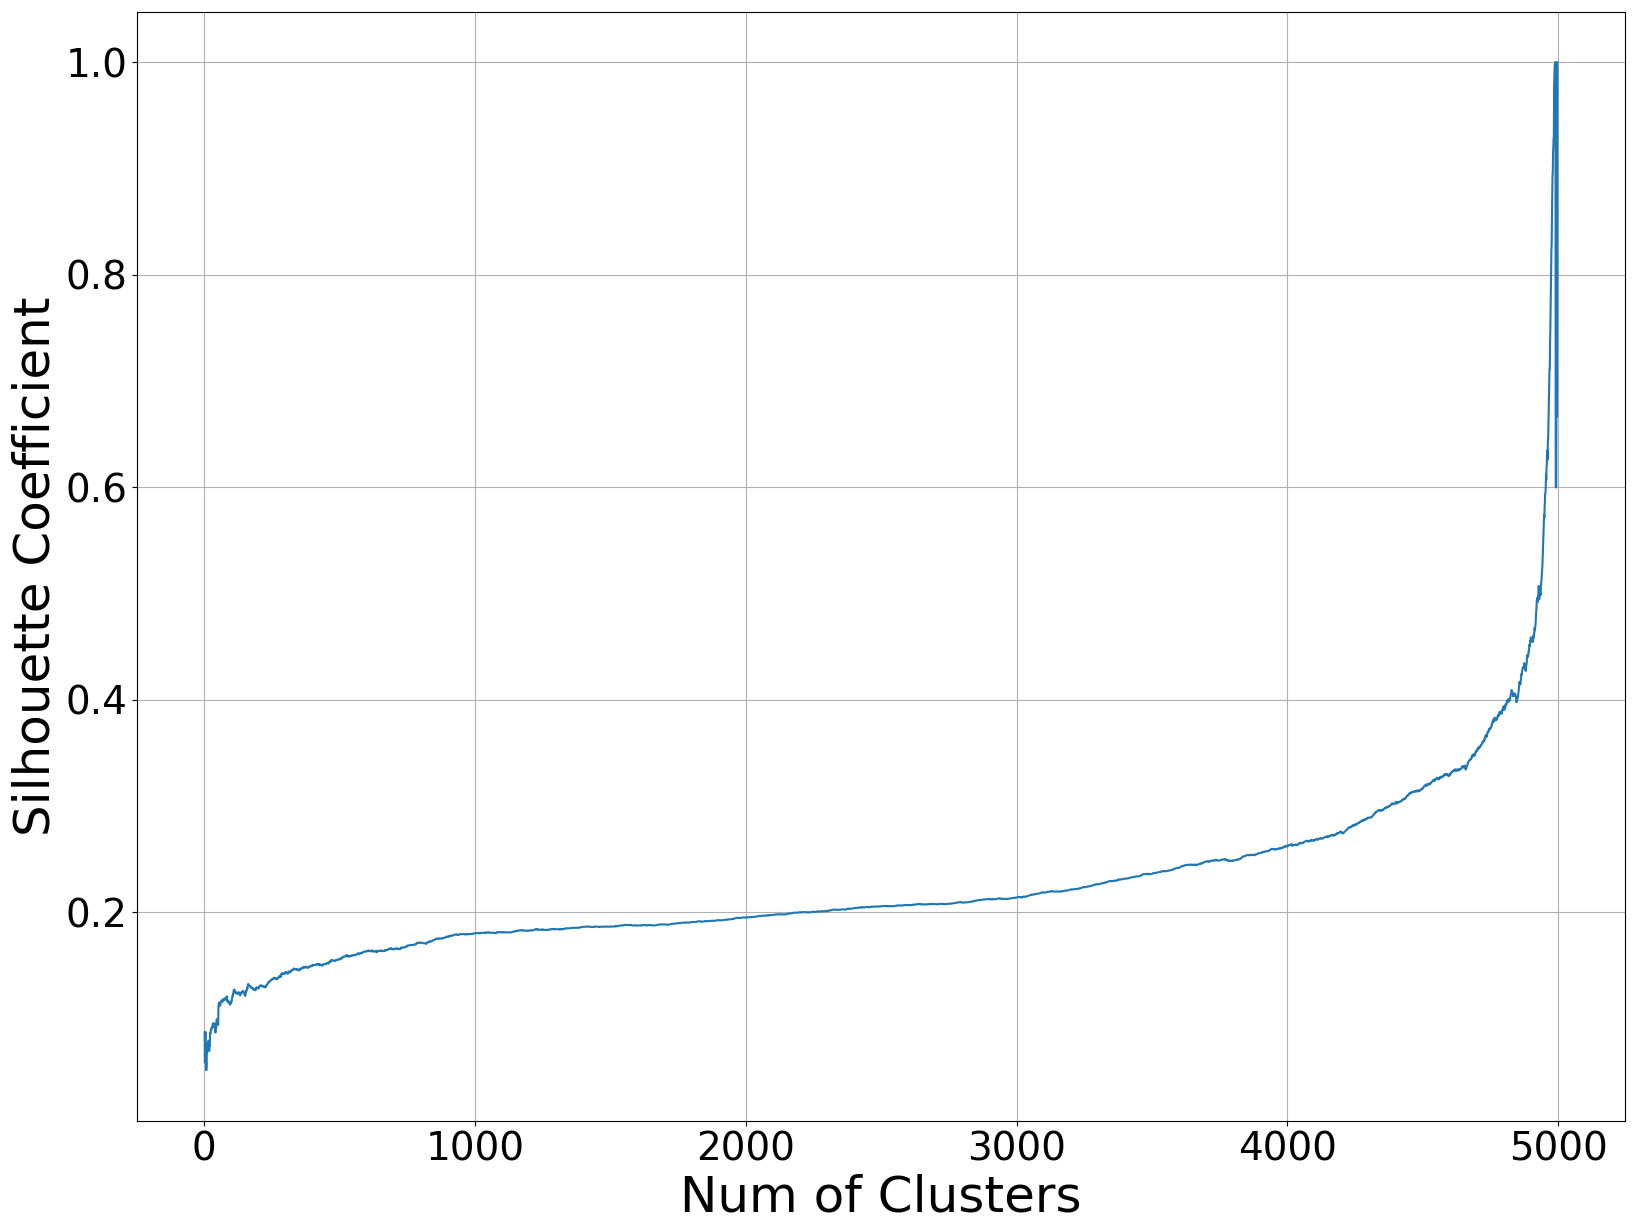
\includegraphics[keepaspectratio, width=120mm]{img/process-06_articles-cluster_num-of-clusters-dependency-on-silhouette-coefficient_with-maximal-silhoette_reduced-data-to-5000_Trim.png}
	\caption{記事の階層的クラスタリングにおけるクラスタ数ごとのシルエット係数}
	\label{articles_silhouette}
\end{figure}

\textcolor{red}{add \textbackslash newpage}
\newpage

図\ref{num_and_size_of_clusters_of_articles}にクラスタを分けるクラスタ間距離ごとにまとめたクラスタ数とクラスタ内の平均記事数を示す.
図\ref{num_and_size_of_clusters_of_articles}の上の図から,クラスタ間距離0.5の付近(クラスタ数2000の付近)でクラスタ間距離を大きくしたときのクラスタ数の減少が緩やかになり始めていることがわかる.
クラスタ数2000から500にかけてはグラフが直線的であったため,小節\ref{subsection_scalable_fact_checking}で述べたYangらのシステムと比較がしやすいクラスタ間距離0.85(クラスタ数666)でクラスタを分割し,以降の実験を行うこととした\cite{yang_scalable_2021}.
クラスタ間距離0.85でのクラスタ内の平均記事数は7.51件であり,読者への異なる主張の提示に適当な量であると考える.

\begin{figure}[H]
	\centering
	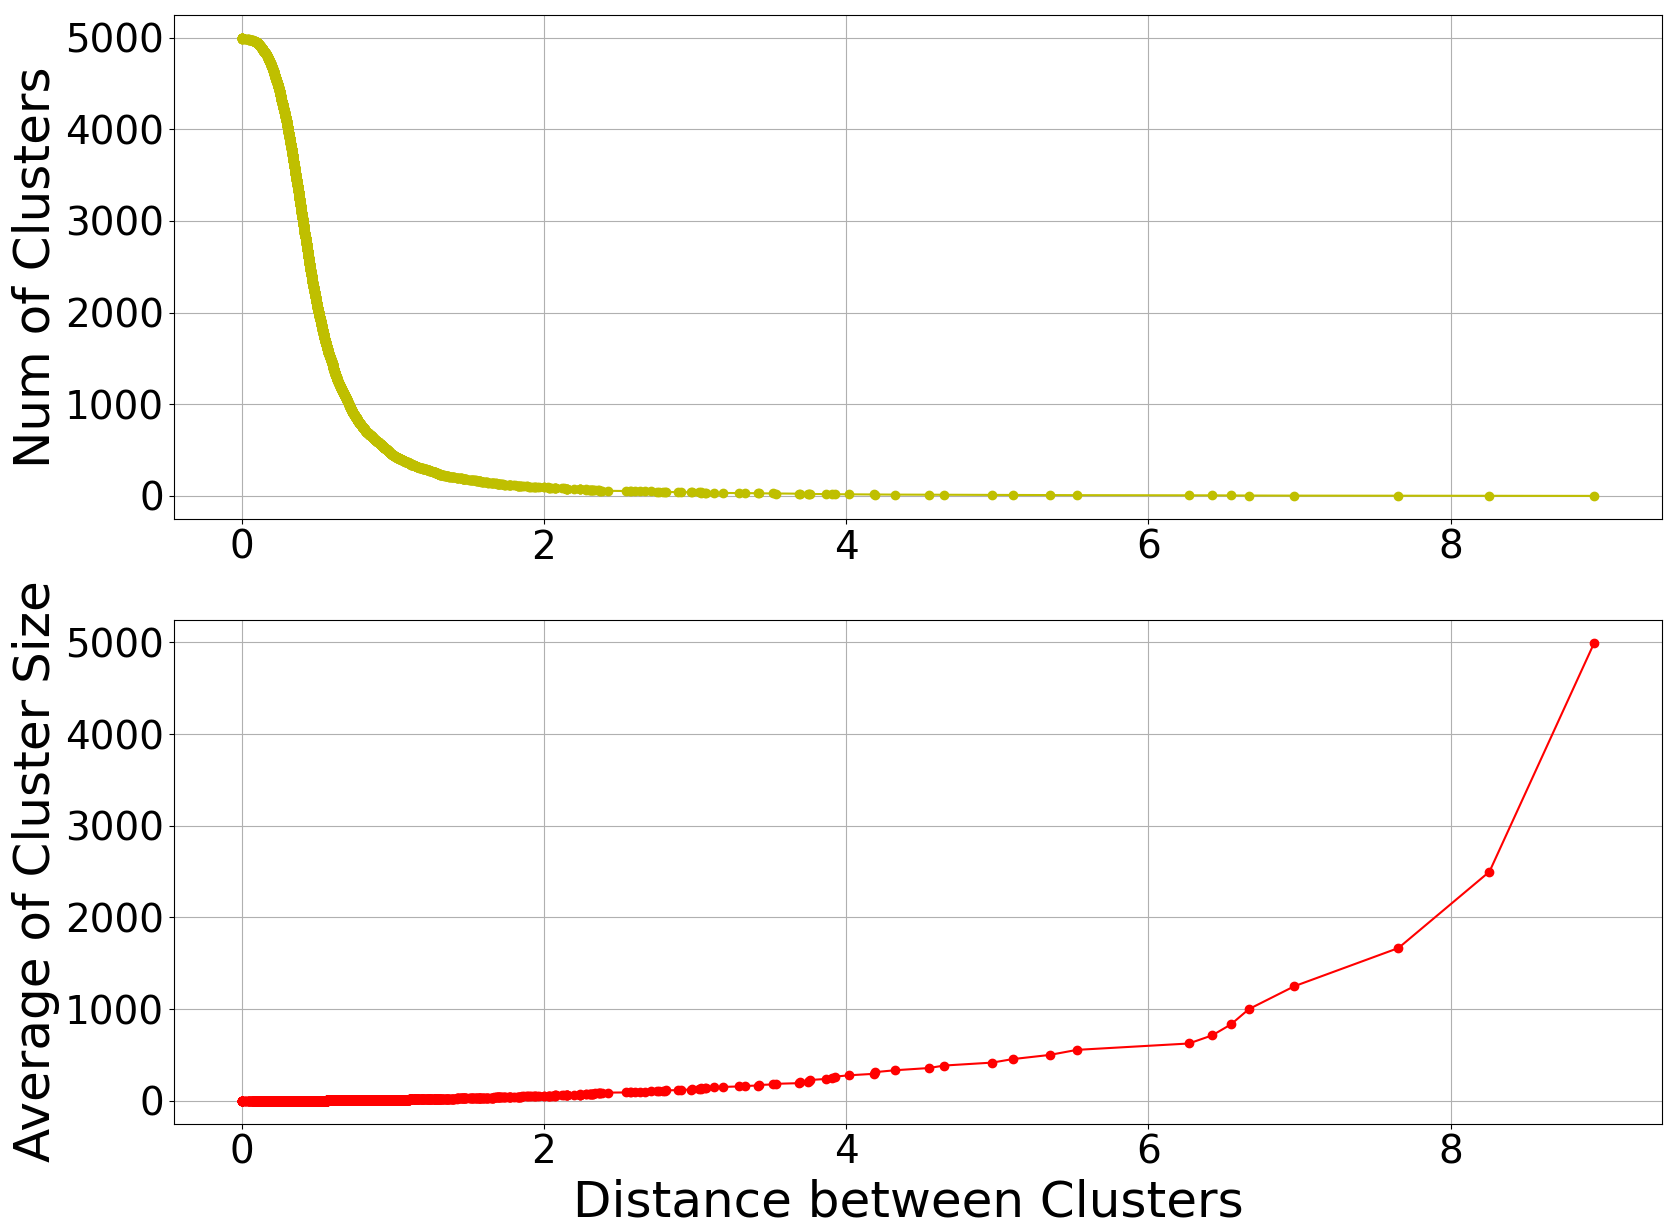
\includegraphics[keepaspectratio, width=120mm]{img/process-06_articles-cluster_threshold-dependencies_reduced-data-to-5000_edit-label_Trim.png}
	\caption{クラスタを分けるクラスタ間距離ごとの「クラスタ数」と
  % \newline
  % \qquad~
  「クラスタ内の平均記事数」}
	\label{num_and_size_of_clusters_of_articles}
\end{figure}

\textcolor{red}{add \textbackslash newpage}
\newpage

図\ref{articles_dendrogram}に記事の階層的クラスタリングの結果をデンドログラムで示す.
クラスタ間距離0.85以下の最後の結合で分かれたクラスタに色を付けている.

\begin{figure}[H]
	\centering
	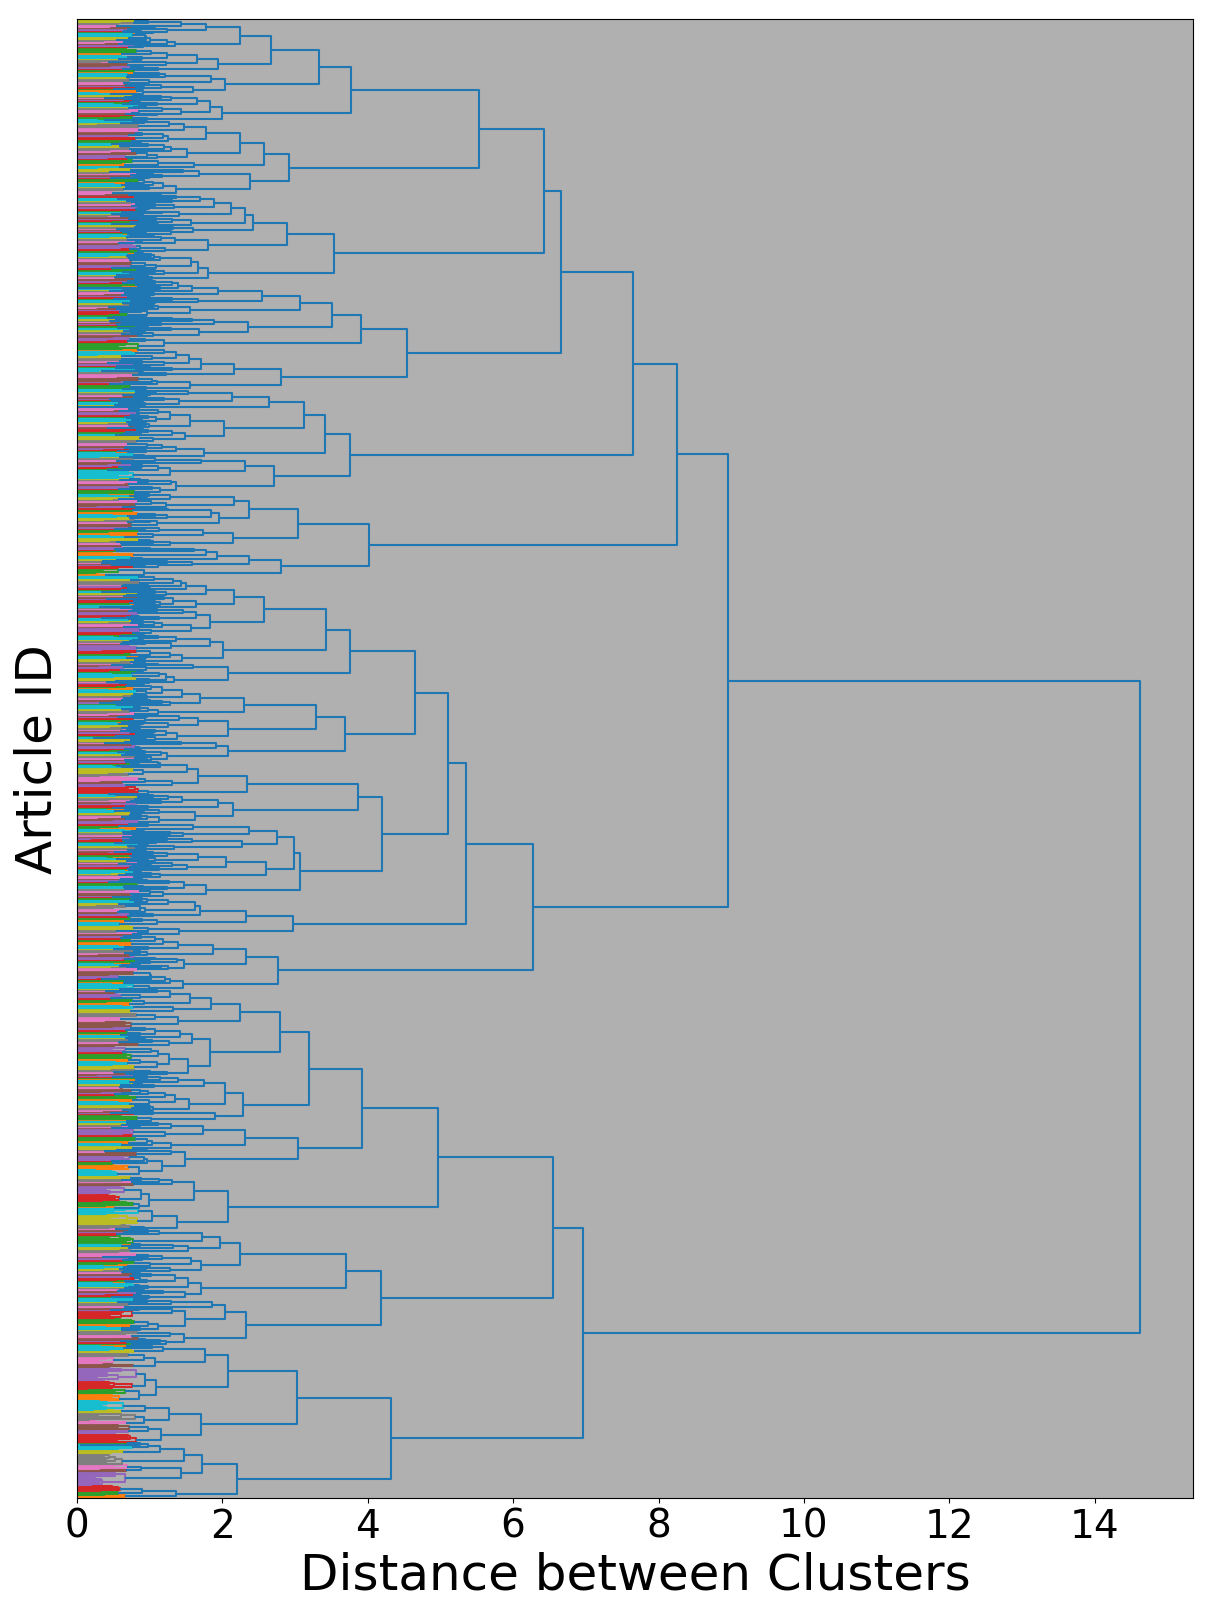
\includegraphics[keepaspectratio, width=120mm]{img/process-06_articles-cluster_color_dendrogram_with-threshold-85_reduced-data-to-5000_Trim.png}
	\caption{記事の階層的クラスタリングの結果}
	\label{articles_dendrogram}
\end{figure}

\textcolor{red}{add \textbackslash newpage}
\newpage

色付けされたクラスタのうち,3ヶ国すべての国の記事を含む最も文字数が多いクラスタを抽出した.
% 記事ID 230
% このクラスタは4番目に文字数が多かった.
このクラスタには38件の記事が属しており,記事の文のうち主張の文は13文であった.
表\ref{articles_clustering_example}にこの13文の主張の文と主張の対象とした出来事を示す.
13文中10文(約77\%)がウイルス感染対策に関する類似した出来事に対して主張を述べる文であった.
また,残りの3文のうち2文はウイルス感染の社会の影響に関する出来事に対して主張を述べる文であり,ウイルス感染対策と出来事が類似している.
% 13文中12文(約92\%)が類似した出来事に対する主張の文であったとも解釈できる.

また,インドから1文,韓国から9文,日本から3文だけ主張の文が抽出されており,異なる地域から主張や記事を提示可能であると期待できる.

\begin{table}[H]
  \caption{1つの記事のクラスタが含む主張の文と主張の対象とした出来事}
  \vspace{4mm}
  \centering
  % {\tabcolsep=0.1cm
  \begin{tabular}{ccp{10cm}}
      \hline
      国 & 出来事 & \multicolumn{1}{c}{記事のクラスタが含む主張の文}
      \\
      \hline
      インド & 仕事 & \baselineskip=16pt
      it was a laborious \textbf{job}.
      \\[1.7mm]
      韓国 & \textbf{感染対策} & \baselineskip=16pt
      sports event are also obligated to \textbf{keep the ceiling of 30 percent at stadiums}.
      \\[1.7mm]
      韓国 & \textbf{感染対策} & \baselineskip=16pt
      south korea operates a threetier \textbf{social distancing} system.
      \\[1.7mm]
      日本 & \textbf{感染対策} & \baselineskip=16pt
      chinese banks have been ordered to \textbf{disinfect} old banknotes before reissuing them to the public.
      \\[1.7mm]
      日本 & \textbf{感染対策} & \baselineskip=16pt
      uncertainly remained over how best to \textbf{stem the spread of the illness}.
      \\[1.7mm]
      日本 & \textbf{感染対策} & \baselineskip=16pt
      \textbf{outdoor exercise will be banned} and \textbf{wearing masks} will be mandatory.
      \\[1.7mm]
      韓国 & \textbf{感染対策} & \baselineskip=16pt
      franchie cafes and dessert shops were obligated to offer \textbf{only takeout around the clock}.
      \\[1.7mm]
      韓国 & \textbf{感染対策} & \baselineskip=16pt
      health authorities remain \textbf{vigilant over sporadic cluster infections} at hospitals nursing homes and riskprone facilities.
      \\[1.7mm]
      韓国 & 感染の影響 & \baselineskip=16pt
      \textbf{travelrelated cases} continue to \textbf{outnumber local cases}.
      \\[1.7mm]
      韓国 & \textbf{感染対策} & \baselineskip=16pt
      to \textbf{keep out imported infections} authorities have \textbf{imposed more stringent measures on people} arriving from countries deemed highrisk.
      \\[1.7mm]
      韓国 & \textbf{感染対策} & \baselineskip=16pt
      cities and provinces that agree to accommodate passengers who require a twoweek \textbf{quarantine} will be paid government incentives.
      \\[1.7mm]
      韓国 & \textbf{感染対策} & \baselineskip=16pt
      \textbf{try not to eat in restaurants} as much as possible.
      \\[1.7mm]
      韓国 & 感染の影響 & \baselineskip=16pt
      the citys \textbf{hospitals} are facing \textbf{an overcrowding crisis}.
      \\[1mm]
      \hline
    \end{tabular}
    \label{articles_clustering_example}
    % }
\end{table}

% IN;24615;8;c;it was a laborious job.
% KR;8909;18;c;sports event are also obligated to keep the ceiling of 30 percent at stadiums.
% KR;8909;19;c;south korea operates a threetier social distancing system.
% JP;13111;30;c;chinese banks have been ordered to disinfect old banknotes before reissuing them to the public.
% JP;13111;34;c;uncertainly remained over how best to stem the spread of the illness.
% JP;20865;22;c;outdoor exercise will be banned and wearing masks will be mandatory.
% KR;3437;15;c;franchise cafes and dessert shops were obligated to offer only takeout around the clock.
% KR;9550;6;c;health authorities remain vigilant over sporadic cluster infections at hospitals nursing homes and riskprone facilities.
% KR;2422;4;c;travelrelated cases continue to outnumber local cases.
% KR;2422;5;c;to keep out imported infections authorities have imposed more stringent measures on people arriving from countries deemed highrisk.
% KR;2422;16;c;cities and provinces that agree to accommodate passengers who require a twoweek quarantine will be paid government incentives.
% KR;2422;27;c;try not to eat in restaurants as much as possible.
% KR;6163;13;c;the citys hospitals are facing an overcrowding crisis.
% @see 

\subsection{実験の考察}
記事の階層的クラスタリングを行った結果,あるクラスタの主張の文の約77\%が類似した出来事に対する主張を述べており,提案手法のシステムで類似した出来事のグループ化が可能であることがわかった.
また,表\ref{articles_clustering_example}で類似した出来事を対象としていると判断した文では``social distancing'',``stem the spread of the illness'',``qurantine''などの異なる単語や動詞句が判断基準となっており,Sentence-BERTによって文の意味や文脈を加味したグループ化ができていることがわかる.

小節\ref{subsection_scalable_fact_checking}で述べたYangらのシステムではシルエット係数の平均値が0.79であり,提案手法のシステムの平均値(約0.17)よりも高い値をとっている\cite{yang_scalable_2021}.
Yangらのシステムでシルエット係数が高い理由は,内容が個々の記事に依存するツイート群を収集しているからであると考える.
つまり,ある1つの記事に対するツイート群で類似したクラスタが形成される傾向にあり,また異なる2つの記事に依存した2つのクラスタはそれぞれ類似しないツイート群で形成される傾向にあるため,シルエット係数が高くなる傾向にあると考えられる.

提案手法のシステムでシルエット係数が低い理由は,出来事の文章の文埋め込みが384次元であるためにシステムが考慮する特徴が多く,極端にデータが類似することや類似しないことがないためだと考えられる.
提案手法では出来事の文章を結合して文埋め込みを作成したが,システムが考慮する特徴が減るように,出来事の文章を要約した1文を抽出もしくは生成して文埋め込みを作成することでシルエット係数の平均値が向上する可能性がある.
% 次元の呪いもある

抽出した記事のクラスタでは10件のウイルス感染対策に関する文とその他3件の文を出来事として区別できていないため,クラスタ間距離の算出方法やクラスタを分けるクラスタ間距離の設定方法などに改善が必要である.
% @see 

%%%%%%%%%%%%%%%%%%%%%%%%%%%%%%
\section{主張の文の階層的クラスタリングの実験}
\label{section_sentence_clustering_experiment}

\subsection{実験方法}
主張の文の階層的クラスタリングの実験には,表\ref{articles_clustering_example}の13件の主張の文を用いる.
文のIDに紐づけられた主張の文の文埋め込みを使用し,コサイン距離とWard法を用いた階層的クラスタリングを行う.

% まず,クラスタを結合する度に全埋め込みのシルエット係数の平均を算出した.
% これにより,クラスタを分けるクラスタ間距離ごとに,同一クラスタ内の埋め込みが類似しているか,異なるクラスタ間の埋め込みが類似していないかを確認した.

% クラスタを分けるクラスタ間距離には,クラスタ間距離を大きくしたときにクラスタ数の減少が緩やかになり始める距離を選択した.
% この距離は,より類似しない文章がクラスタにまとめられ始めるクラスタ間距離に対応する.
% このクラスタ間距離を同定するため,結合するクラスタ間距離ごとのクラスタの数をグラフに表した.
% また,このクラスタ間距離でクラスタごとの記事の数が読者の把握できる量を超えていないか確認するため,結合するクラスタ間距離ごとのクラスタがもつ平均の記事の数をグラフに表した.

記事の階層的クラスタリングと同様に全埋め込みのシルエット係数の平均値を算出し,クラスタ間距離ごとのクラスタの数とクラスタがもつ主張の文の数の平均値をグラフに表した.
その後,クラスタを分けるクラスタ間距離としてクラスタ数の減少が緩やかになり始める距離を選択した.

階層的クラスタリングを行った後,それぞれのクラスタに属する文章を目視で確認し,クラスタ内の主張の文が類似しているかを分析した.また,異なるクラスタ間で文が類似しないシステムになっているかを分析した.
% また,抽出したクラスタ内の主張の文のうちの,類似した出来事について述べている文の割合を算出した.

% @see 

\textcolor{red}{add \textbackslash newpage}
\newpage

\subsection{実験結果}

図\ref{sentences_silhouette}にクラスタ数ごとのシルエット係数を示す.
シルエット係数が常に0より大きいため,同一クラスタ内の文埋め込みが類似し,異なるクラスタ間の文埋め込みが類似していない傾向にあることがわかる.
クラスタ数が9から12の範囲ではシルエット係数は大きいが,1つのクラスタ内の主張の文の数が1, 2件であることが多く,類似した主張の文をグループ化できていない可能性がある.
クラスタ数が2から8の範囲ではシルエット係数に大きな差がないため,この範囲でクラスタを分けるクラスタ間距離の設定を考える.

\begin{figure}[H]
	\centering
	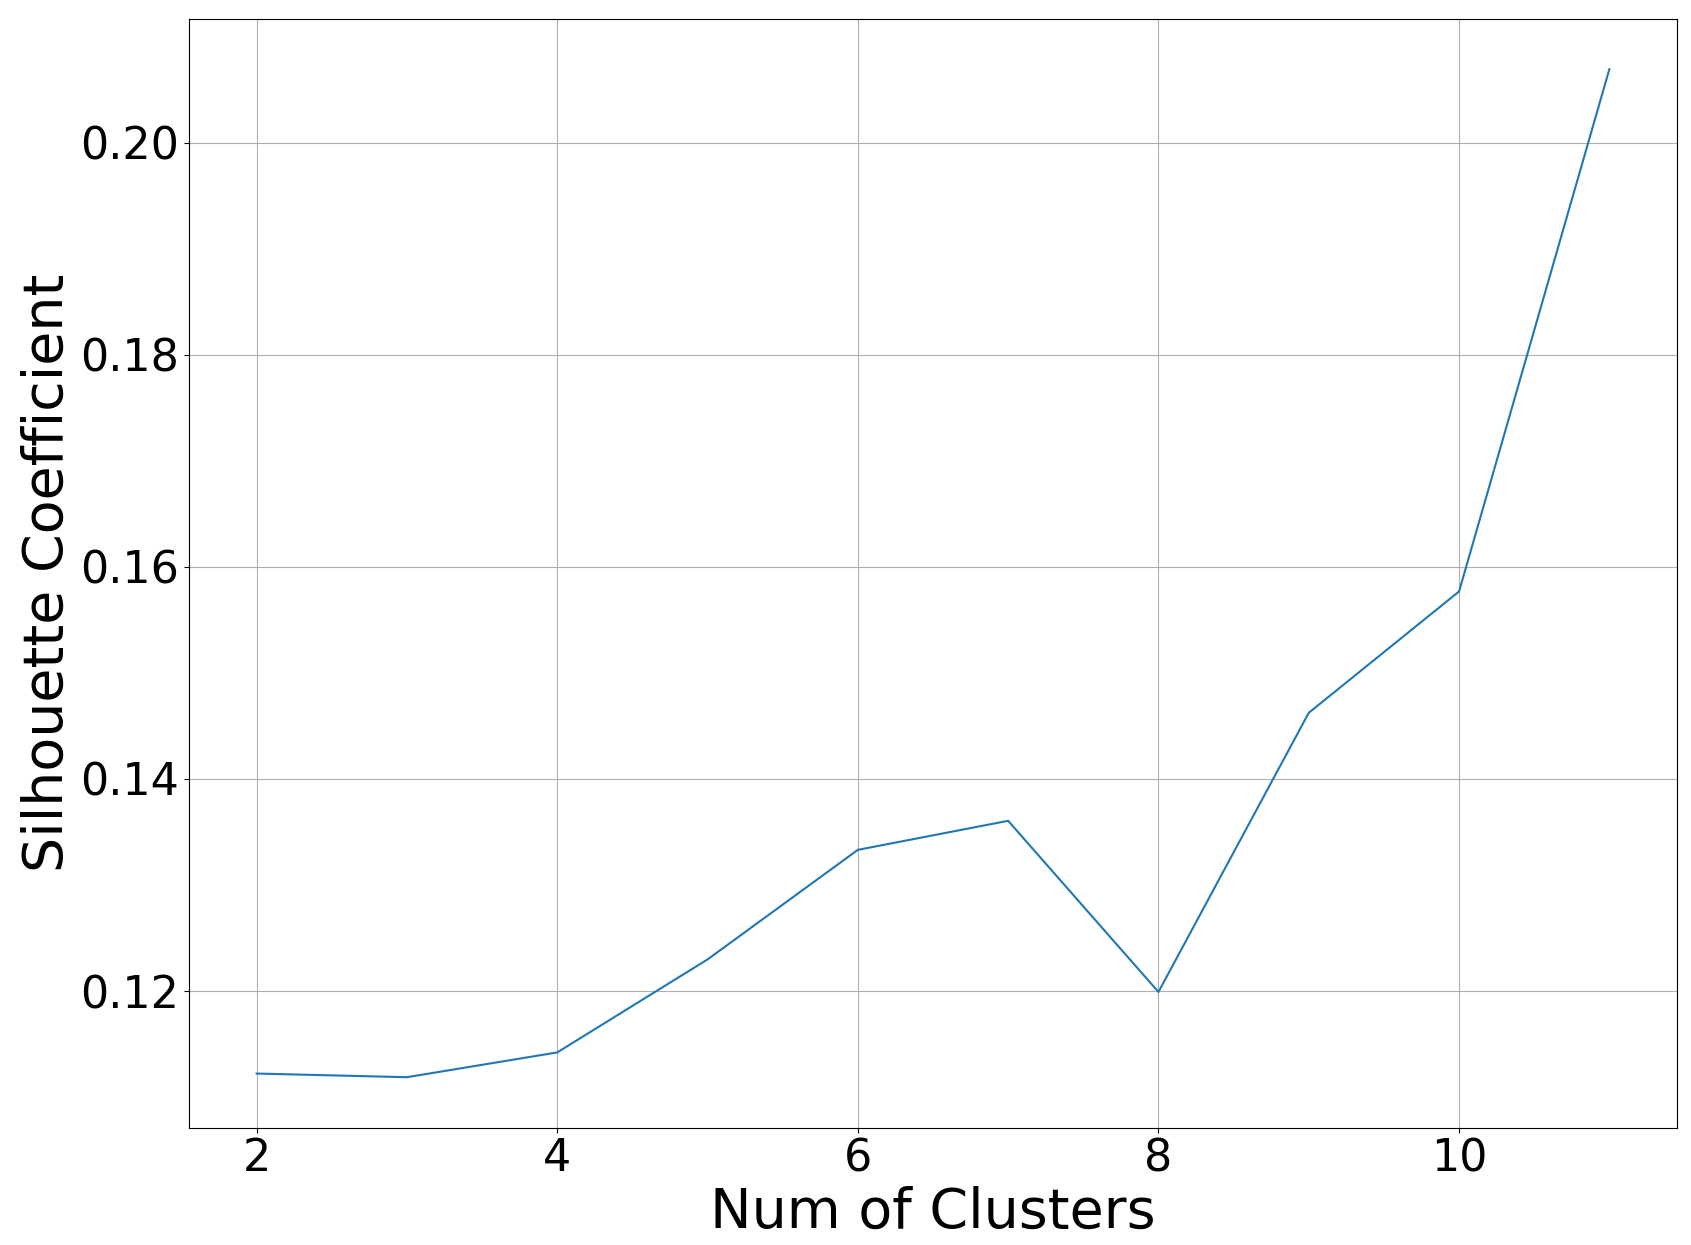
\includegraphics[keepaspectratio, width=120mm]{img/process-07_sentences-cluster_from-cluster-230_with-threshold-85_num-of-clusters-dependency-on-silhouette-coefficient_reduced-data-to-5000_Trim.png}
	\caption{主張の文の階層的クラスタリングにおけるクラスタ数ごとのシルエット係数}
	\label{sentences_silhouette}
\end{figure}

\textcolor{red}{add \textbackslash newpage}
\newpage

図\ref{num_and_size_of_clusters_of_sentences}にクラスタを分けるクラスタ間距離ごとにまとめたクラスタ数とクラスタ内の主張の文の数の平均値を示す.
図\ref{num_and_size_of_clusters_of_sentences}の上の図から,クラスタ間距離0.85の付近(クラスタ数2000の付近)でクラスタ間距離を大きくしたときのクラスタ数の減少が緩やかになり始めていることがわかる.
このクラスタ間距離は小節\ref{subsection_scalable_fact_checking}で述べたYangらのシステムで用いた値と一致しており,比較評価がしやすい\cite{yang_scalable_2021}.
したがって,このクラスタ間距離0.85(クラスタ数5)でクラスタを分割し,以降の実験を行うこととした.
クラスタ間距離0.85でのクラスタ内の主張の文の数の平均値は2.6文であり,類似した主張の文をグループ化できている可能性がある.

\begin{figure}[H]
	\centering
	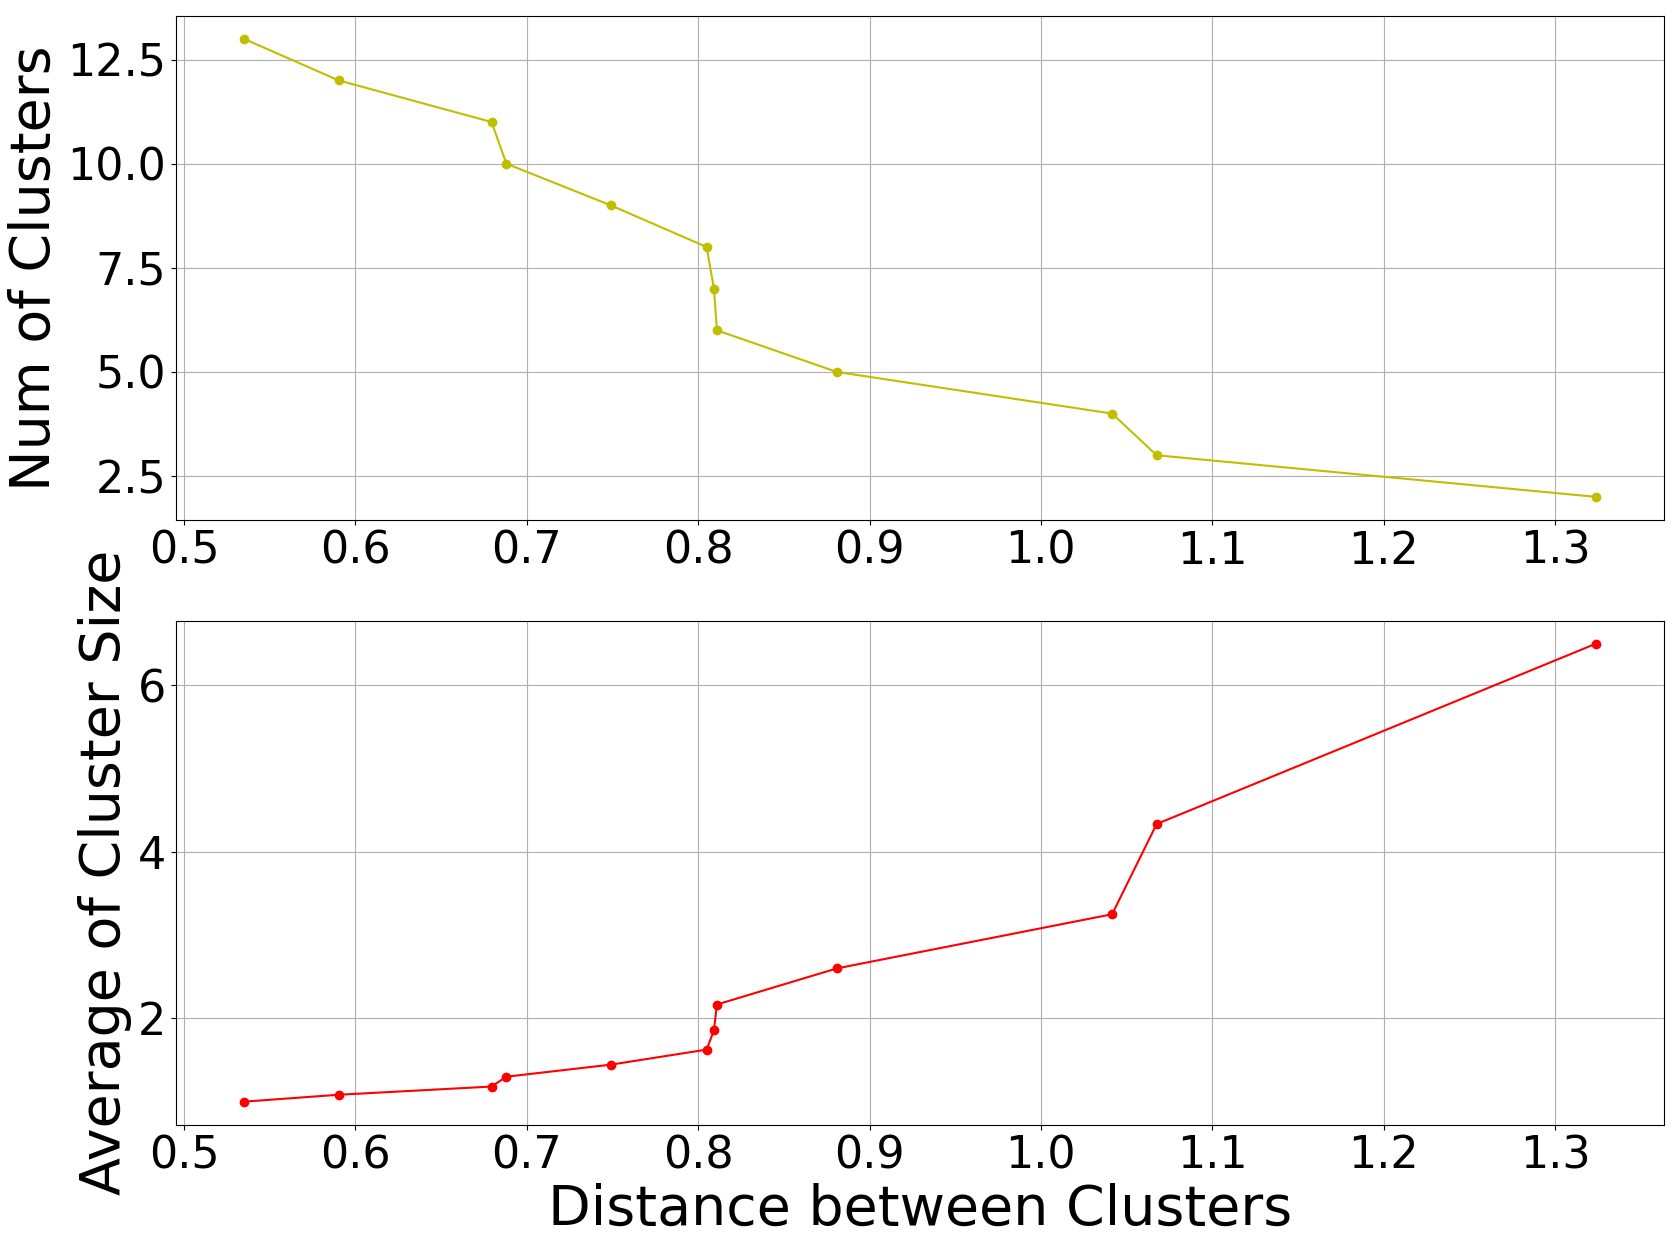
\includegraphics[keepaspectratio, width=120mm]{img/process-07_sentences-cluster_from-cluster-230_with-threshold-85_threshold-dependencies_reduced-data-to-5000_Trim.png}
	\caption{クラスタを分けるクラスタ間距離ごとの「クラスタ数」と
  % \newline
  % \qquad~
  「クラスタ内の主張の文の数の平均値」}
	\label{num_and_size_of_clusters_of_sentences}
\end{figure}

\textcolor{red}{add \textbackslash newpage}
\newpage

図\ref{sentences_dendrogram}に主張の文の階層的クラスタリングの結果をデンドログラムで示す.
クラスタ間距離0.85以下の最後の結合で分かれたクラスタに色を付けている.

\begin{figure}[H]
	\centering
	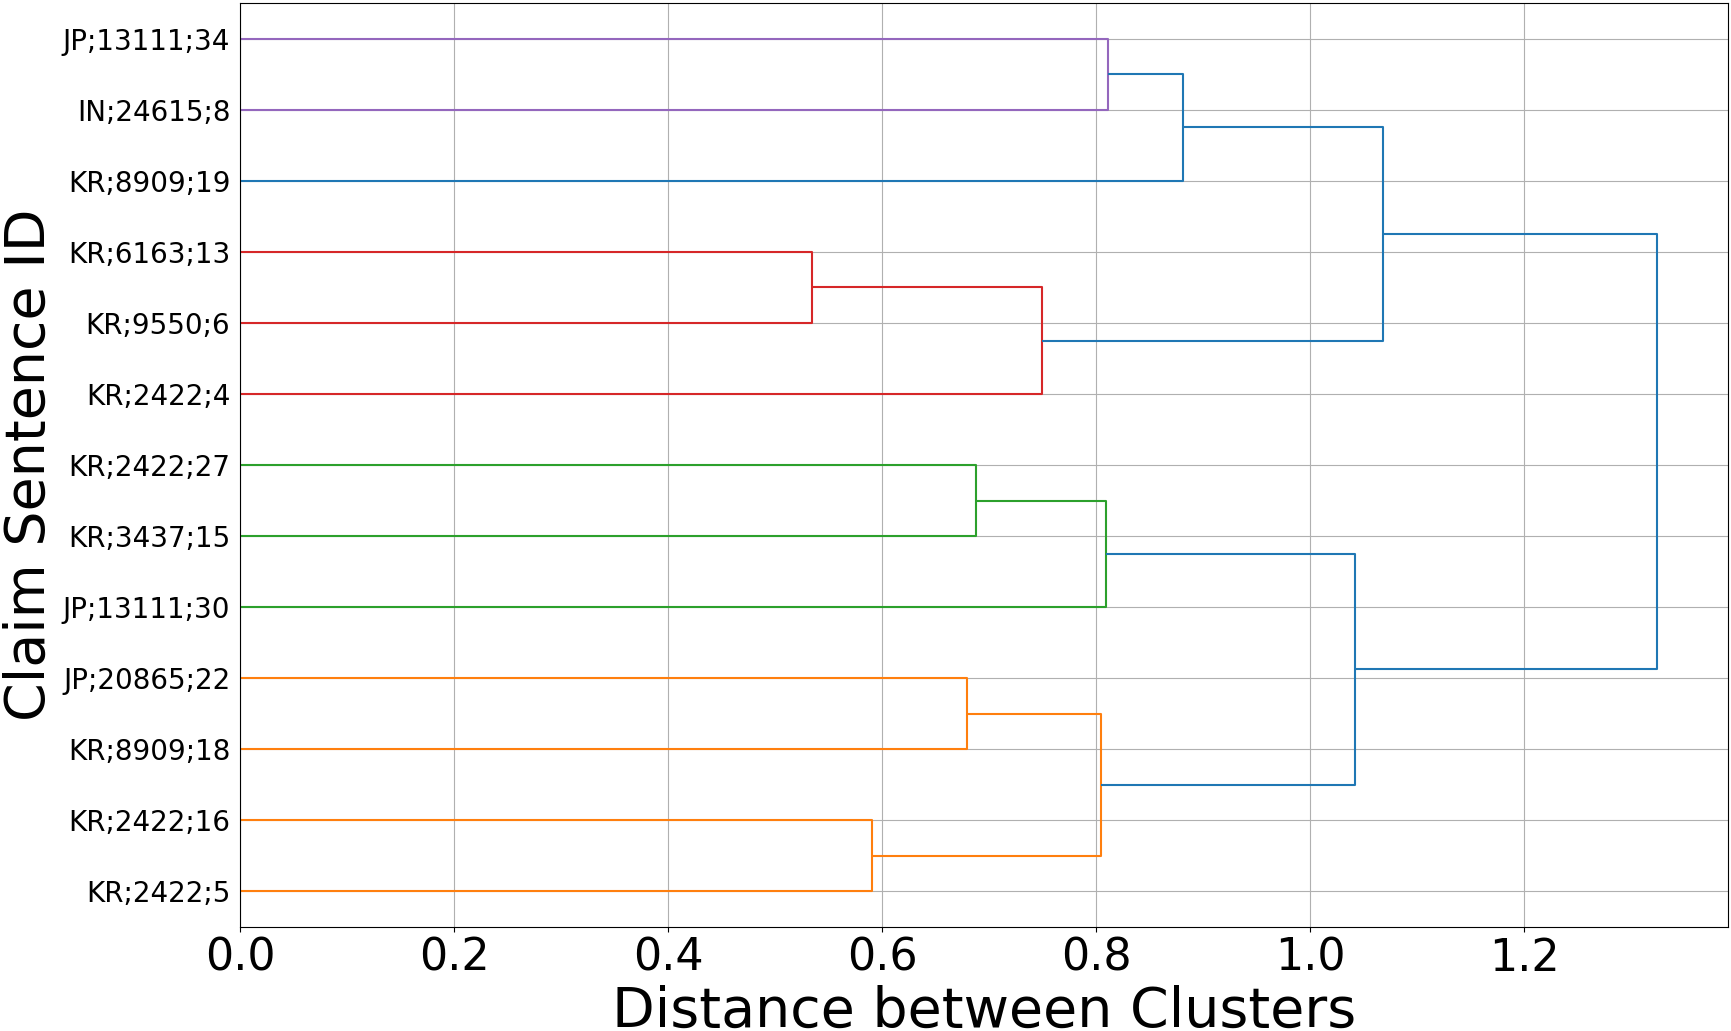
\includegraphics[keepaspectratio, width=120mm]{img/process-07_sentences-cluster_from-cluster-230_with-threshold-85_color_dendrogram_reduced-data-to-5000_y-120_Trim.png}
	\caption{記事の階層的クラスタリングの結果}
	\label{sentences_dendrogram}
\end{figure}

表\ref{sentences_clustering_example}に13文の主張の文と主張の対象とした出来事をクラスタごとに示す.
クラスタ内外の主張の文の類似度を確認するため,主張の文が対象にしている出来事について,その対象とする事物をまとめた.

図\ref{sentences_dendrogram}で緑色に色付けしたクラスタには3文中2文が飲食店での感染対策に関する類似した主張がグループ化されていた.
また,図\ref{sentences_dendrogram}で黄色に色付けしたクラスタには4文中2文が運動時の感染対策に関して,残りの2文が旅行時の感染対策に関しての主張がグループ化されていた.
このことから,同一のクラスタ内で類似した主張の文が集まり,5000件の記事の主張が要約できていることがわかる.

一方で,異なるクラスタ間で出来事とその対象の組が一致する文は1つもなく,異なるクラスタに異なる主張の文が属していることがわかる.
これらの文は出来事だけ見れば13文中10文(約77\%)が感染対策に関する類似した出来事に対して主張を述べる文であるため,提案手法で類似した出来事の異なる主張を提示できることがわかった.

\begin{table}[H]
  \caption{クラスタごとの主張の文と主張の対象とした出来事}
  \vspace{4mm}
  \centering
  % {\tabcolsep=0.15cm
  \begin{tabular}{p{2.7cm}p{1.6cm}cp{6.8cm}}
      \hline
      \baselineskip=16pt 所属クラスタの図\ref{sentences_dendrogram}での色 &
      \baselineskip=16pt 出来事の対象 &
      \hfil \multirow{1}{*}[-2mm]{\shortstack{出来事}} &
      \hfil \multirow{1}{*}[-2mm]{\shortstack{主張の文}}
      \\
      \hline
      \hline
      \multicolumn{1}{c}{紫} & \multicolumn{1}{c}{-} & \textbf{感染対策} & \baselineskip=16pt
      uncertainly remained over how best to \textbf{stem the spread of the illness}.
      \\[2mm]
      \multicolumn{1}{c}{紫} & \multicolumn{1}{c}{-} & 仕事 & \baselineskip=16pt
      it was a laborious \textbf{job}.
      \\[2mm]
      \hline
      \multicolumn{1}{c}{青} & \multicolumn{1}{c}{国の全域} & \textbf{感染対策} & \baselineskip=16pt
      \textbf{south korea} operates a threetier \textbf{social distancing} system.
      % \hline
      \\[2mm]
      \hline
      \multicolumn{1}{c}{赤} & \multicolumn{1}{c}{病院} & 感染の影響 & \baselineskip=16pt
      the citys \textbf{hospitals} are facing \textbf{an overcrowding crisis}.
      \\[2mm]
      \multicolumn{1}{c}{赤} & \multicolumn{1}{c}{病院など} & \textbf{感染対策} & \baselineskip=16pt
      health authorities remain \textbf{vigilant over sporadic cluster infections} at \textbf{hospitals nursing homes and riskprone facilities}.
      \\[2mm]
      \multicolumn{1}{c}{赤} & \multicolumn{1}{c}{旅行} & 感染の影響 & \baselineskip=16pt
      \textbf{travelrelated cases} continue to \textbf{outnumber local cases}.
      \\[2mm]
      \hline
      \multicolumn{1}{c}{緑} & \textbf{飲食店} & \textbf{感染対策} & \baselineskip=16pt
      \textbf{try not to eat in restaurants} as much as possible.
      \\[2mm]
      \multicolumn{1}{c}{緑} & \textbf{飲食店} & \textbf{感染対策} & \baselineskip=16pt
      \textbf{franchie cafes} and \textbf{dessert shops} were obligated to offer \textbf{only takeout around the clock}.
      \\[2mm]
      \multicolumn{1}{c}{緑} & 銀行 & \textbf{感染対策} & \baselineskip=16pt
      chinese \textbf{banks} have been ordered to \textbf{disinfect} old banknotes before reissuing them to the public.
      \\[1mm]
    \end{tabular}
    \label{sentences_clustering_example}
    % }
  \end{table}
  
  \newpage
  
  
  \begin{table}[H]
    % \caption{クラスタごとの主張の文と主張の対象とした出来事}
    % \vspace{4mm}
    \centering
  % {\tabcolsep=0.15cm
    \begin{tabular}{p{2.7cm}ccp{6.8cm}}
      % \hline
      % 所属クラスタの図\ref{sentences_dendrogram}での色 & 出来事1 & 出来事2 & \multicolumn{1}{c}{主張の文}
      % \\
      % \hline
      \hline
      \multicolumn{1}{c}{黄} & \textbf{運動} & \textbf{感染対策} & \baselineskip=16pt
      \textbf{outdoor exercise will be banned} and \textbf{wearing masks} will be mandatory.
      \\[2mm]
      \multicolumn{1}{c}{黄} & \textbf{運動} & \textbf{感染対策} & \baselineskip=16pt
      \textbf{sports event} are also obligated to \textbf{keep the ceiling of 30 percent at stadiums}.
      \\[2mm]
      \multicolumn{1}{c}{黄} & \textbf{旅行} & \textbf{感染対策} & \baselineskip=16pt
      cities and provinces that agree to accommodate \textbf{passengers} who require a twoweek \textbf{quarantine} will be paid government incentives.
      \\[2mm]
      \multicolumn{1}{c}{  ~~黄~~  } &  \textbf{旅行}  & \textbf{~感染対策~} & \baselineskip=16pt
      to \textbf{keep out imported infections} authorities have \textbf{imposed more stringent measures on people arriving from countries deemed highrisk}.
      \\[1mm]
      \hline
    \end{tabular}
    % }
\end{table}


% @see 

\subsection{実験の考察}
表\ref{sentences_clustering_example}の分析から,提案手法で類似した出来事の異なる主張を提示できることがわかった.
しかし,緑色のクラスタは飲食店と銀行を出来事の対象として分割できておらず,黄色のクラスタは運動と旅行を出来事の対象として分割できていない.
したがって,同一クラスタ内の主張の文をより類似した文のみでグループ化したいときは,クラスタ間距離の算出方法やクラスタを分けるクラスタ間距離の設定方法などに改善が必要である.

小節\ref{subsection_scalable_fact_checking}で述べたYangらのシステムでは959件の記事の主張を705個の「出来事が混在した異なる主張のクラスタ」(約74\%)に要約していたのに対し,提案手法のシステムでは5000件の記事の主張を5個の「類似した出来事の異なる主張のクラスタ」(0.5\%)に要約できた.
これにより,読者が興味を持っている出来事の異なる主張の収集に時間を要してしまうYangらのシステムの問題は,提案手法のシステムで改善できたと考える.

本実験での主張の文の階層的クラスタリングの評価は,1つの記事のクラスタが含む13件の主張の文で行った.
類似した出来事の異なる主張を提示できるかの評価をより信頼できるものにするためには,他のより多くの記事のクラスタでの評価や入力する記事の数を増やしたときの評価,データセットを変えたときの評価などが必要である.

% 出来事をやらずに主張だけクラスタリングしたら面白そう
% @see 


% %%%%%%%%%%%%%%%%%%%%%%%%%%%%%%%%%%%%%%%%%%%%%%%%%%%%%%%%%%%%
% \chapter{結果と考察}
% %%%%%%%%%%%%%%%%%%%%%%%%%%%%%%%%%%%%%%%%%%%%%%%%%%%%%%%%%%%%


% %%%%%%%%%%%%%%%%%%%%%%%%%%%%%%
% \section{既存手法との比較}
% ~
% % @see 

% %%%%%%%%%%%%%%%%%%%%%%%%%%%%%%
% \section{提案手法の妥当性}
% ~
% % @see 

% \subsection{入力と出力の妥当性}
% ~
% % @see 

% \subsection{処理速度の妥当性(分散システムの議論も)}
% ~
% % @see 

% %%%%%%%%%%%%%%%%%%%%%%%%%%%%%%
% \section{(結果を基に検討)}
% ~
% % @see 

%%%%%%%%%%%%%%%%%%%%%%%%%%%%%%%%%%%%%%%%%%%%%%%%%%%%%%%%%%%%
\chapter{まとめと今後の課題}
%%%%%%%%%%%%%%%%%%%%%%%%%%%%%%%%%%%%%%%%%%%%%%%%%%%%%%%%%%%%
\label{chapter_conclusion}

%%%%%%%%%%%%%%%%%%%%%%%%%%%%%%
% \section{まとめ}
本研究では出来事の文(Evidenceの文)と主張の文(Claimの文)のクラスタを用いた多様な主張を提示するニュース推薦手法を提案した.
より類似した出来事の異なる主張の文を提示するため,記事の文を出来事の文か主張の文かで分類し,出来事の文章と主張の文の文埋め込みを生成し,それぞれの埋め込みに基づいて記事の階層的クラスタリングと主張の文の階層的クラスタリングを行った.
その後,読者が興味を持っている1つの記事に対し,k-NN分類法を用いてその記事と類似した出来事を扱う主張の文のクラスタを提示し,主張の文に紐づく記事を推薦する手法を提案した.

出来事の文と主張の文の分類器には,事前学習されたRoBERTa baseモデルに1層の全結合層と1ノードの出力層を接続したモデルを使用した.
このモデルの転移学習にはIBM Debater$^{\textregistered}$ - Claims and Evidenceの前処理したEvidenceの文とClaimの文を入力し,損失関数としてバイナリクロスエントロピーを用いた.
文埋め込みの生成にはSentence-BERTのparaphrase-MiniLM-L6-v2モデルを利用し,提案システムが文の意味と文脈を加味できるようにした.
階層的クラスタリングでは文埋め込み間のコサイン距離を用いたWard法によるクラスタ間距離を使用した.

実験では,主張の文の階層的クラスタリングまでを行うシステムを実装し,より類似した出来事の異なる主張の文を提示できているかを評価した.
分類器や階層的クラスタリングの入力にはCOVID-19 News Articlesの5000件の英語の記事を使用し,政治や文化の違いに由来する3ヶ国の多様な主張が分析できるようにした.

IBM Debater$^{\textregistered}$ - Claims and Evidenceを用いた分類器の実験では,適合率が0.86~0.90,再現率が0.89~0.92,マシューズ相関係数が0.82~0.84である4種類のエポック数の精度の高い分類器を作成することができた.しかし,バイナリクロスエントロピーが1エポックから単調増加しており過学習となっている可能性があったため,次の実験では4つのモデルで比較評価を行った.

COVID-19 News Articlesを用いた分類器の実験では,163文の正解ラベルを作成し,このラベルに基づいて適合率が1.00となる分類器を作成することができた.
しかし,再現率が0.40,マシューズ相関係数が0.61と低いため,今後の課題として構文を加味した分類器の作成や記事に適した学習用データセットの検討,過学習しにくいモデルの検討が必要である.
% 文の数とアノテータの話は省略

記事の階層的クラスタリングの実験では,クラスタ間距離0.85以下の最後の結合によって5000件の記事を666個のクラスタに分割した.
ある記事のクラスタでは主張の文の約77\%が類似した出来事に対する主張を述べており,提案手法で類似した出来事のグループ化が可能であることがわかった.
抽出した記事のクラスタでは,77\%の主張の文と23\%の主張の文とで対象とする出来事が類似していなかったため,今後の課題としてクラスタ間距離の算出方法やクラスタを分けるクラスタ間距離の設定方法などに改善が必要である.

主張の文の階層的クラスタリングの実験では,クラスタ間距離0.85以下の最後の結合により,666個の記事のクラスタが含む13件の主張の文を5個のクラスタに分割した.
ある主張の文のクラスタ内では3文中2文が類似した出来事に対して主張を述べており,一方で任意の異なるクラスタ間で出来事とその対象の組が一致する主張の文は1つも存在しなかった.
このことから,提案手法で類似した出来事の異なる主張の提示が可能であることがわかった.
また,小節\ref{subsection_scalable_fact_checking}で述べたYangらのシステムでは959件の記事の主張を705個の「出来事が混在した異なる主張のクラスタ」(約74\%)に要約していたのに対し,提案手法のシステムでは5000件の記事の主張を5個の「類似した出来事の異なる主張のクラスタ」(0.5\%)に要約できた.
これにより,読者が興味を持っている出来事の異なる主張の収集に時間を要してしまうYangらの手法の問題は,提案手法で改善できたと考える.
今後の課題として,同一クラスタ内の主張の文をより類似した文のみでグループ化するために,クラスタ間距離の算出方法やクラスタを分けるクラスタ間距離の設定方法などの改善が必要である.

全体として,より信頼性の高い評価のために,作成する正解ラベルの数や入力する記事の数を増やす必要がある.また,今回実験を行わなかったk-NN分類法を用いた記事の推薦についてもその妥当性を評価する必要がある.

% @see 

%%%%%%%%%%%%%%%%%%%%%%%%%%%%%%
% \section{今後の展望}
% %% @see 
% \section{データセットの相性(ディベートとニュース)}
% ~
% @see 

%%%%%%%%%%%%%%%%%%%%%%%%%%%%%%%%%%%%%%%%%%%%%%%%%%%%%%%%%%%%
\chapter*{謝辞}
\addcontentsline{toc}{chapter}{謝辞}
%%%%%%%%%%%%%%%%%%%%%%%%%%%%%%%%%%%%%%%%%%%%%%%%%%%%%%%%%%%%

本論文の執筆には,非常に多くの方々の支えがありました.
指導教員である木村先生には研究内容に関する議論をはじめとし,勉強会,論文執筆,発表資料作成でのご助言など,大変多くのご助力をいただきました.
先生との研究活動を通し,社会や技術の問題点を発見し解決策を吟味する力が磨かれるなど,人間的に成長することができました.

同じ研究室の大学院生である加瀬裕也さんと疋田智也さんにも,研究活動の様々な場面で多くのご助力をいただきました.
加瀬さんに研究活動の詳細なスケジュールを作成していただいたことで,
円滑な研究活動を行うことができました.
疋田さんに発表資料や本論文を細かく査読していただいたことで
,より相手に伝わりやすい文章を作成することができました.

同じ研究室の学部4年生の方々とは建設的な勉強会を行うことができ,勉強会から多くの研究のヒントを得ることができました.
また,彼ら・彼女らとともに幾度も発表練習を行ったことで,より良い発表を行うことができました.

両親には本学での大学生活を金銭面,生活面で支えてもらい,また多くの悩み事を聞いてもらいました.

ご多忙な日々の中,貴重な時間を割いていただいた皆さまに心から感謝申し上げます.
% @see 先輩の論文,テキスト


%%%%%%%%%%%%%%%%%%%%%%%%%%%%%%%%%%%%%%%%%%%%%%%%%%%%%%%%%%%%
\bibliographystyle{junsrt}
\bibliography{ref.bib}
%%%%%%%%%%%%%%%%%%%%%%%%%%%%%%%%%%%%%%%%%%%%%%%%%%%%%%%%%%%%

\end{document}
